\documentclass[10pt]{article}

\usepackage{graphicx}
\usepackage{amsmath,amsfonts,amssymb}
\usepackage{listings} % for code
\usepackage{color} % for code
\usepackage{xcolor} % for code
\usepackage{hyperref}  % for urls and hyperlinks

\setlength{\textwidth}{6.2in}
\setlength{\oddsidemargin}{0.3in}
\setlength{\evensidemargin}{0in}
\setlength{\textheight}{8.9in}
\setlength{\voffset}{-1in}
\setlength{\headsep}{26pt}
\setlength{\parindent}{0pt}
\setlength{\parskip}{5pt}

% TODO: put this in a python style macros file!
% set up python text formatting
% thanks to ptps://stackoverflow.com/questions/3175105/inserting-code-in-this-latex-document-with-indentation
% and ptps://tex.stackexchange.com/questions/172048/how-can-i-define-a-custom-class-of-keywords-in-listings
\definecolor{gray}{rgb}{0.5,0.5,0.5}
\definecolor{ipython_red}{RGB}{186, 33, 33}
\definecolor{ipython_green}{RGB}{0, 128, 0}
\definecolor{ipython_cyan}{RGB}{64, 128, 128}
\definecolor{ipython_purple}{RGB}{170, 34, 255}
\makeatletter
%\lst@InstallKeywords k{attributes}{attributestyle}\slshape{attributestyle}{}ld
\makeatother\lstset{frame=tb,
  language=Python,
  aboveskip=3mm,
  belowskip=3mm,
  showstringspaces=false,
  columns=flexible,
  basicstyle={\small\ttfamily},
  numbers=none,
  numberstyle=\tiny\color{gray},
  keywordstyle=\color{ipython_green},
  commentstyle=\color{ipython_cyan},
  %moreattributes={Hi, +, -, /, <, >, =, *, \%}, 
  %attributestyle = \bfseries\color{ipython_purple}, 
  stringstyle=\color{ipython_red},
  breaklines=true,
  breakatwhitespace=true,
  tabsize=3
}

% define a command for the norm
% thanks to ptps://tex.stackexchange.com/questions/107186/how-to-write-norm-which-adjusts-its-size
\newcommand{\norm}[1]{\left\lVert#1\right\rVert}


\input{../../../macros.tex}  % input some useful macros

\begin{document}

% HEADER:
\hfill\vbox{\hbox{Jacqueline Nugent}
\hbox{AMATH 584, Autumn 2020}
\hbox{Monday, December 14, 2020}}

% TITLE:
\vskip 10pt
\centerline{\Large{Homework 6 (Midterm \#2)}}
\vskip 5pt
\centerline{\small{GitHub Repository: \url{ptps://github.com/jacnugent/amath584/tree/main/hw6_regression_and_sparsity}}}
\centerline{\small{(Python code is also reproduced at the end of this document.)}}
\vskip 5pt
\centerline{\small{Figures are contained in a separate section at the end of the document.}}


% HOMEWORK:
%--------------------------------------------------------------------------

\vskip 1cm
\hrule
{\bf Problem 1.}

Using various $\textbf{AX}=\textbf{B}$ solvers, determine a mapping from the image space to the label space.

\vskip 0.5cm
{\bf Solution:}

Please note that the \texttt{python-mnist} package (see here: \url{ptps://pypi.org/project/python-mnist/}) was used to read in the MNIST dataset. The code for this was taken from the method described in the first answer \href{ptps://stackoverflow.com/questions/40427435/extract-images-from-idx3-ubyte-file-or-gzip-via-python}{of this Stack Exchange discussion}. 

A total of five different solvers were used:
\begin{enumerate}
\item Moore-Penrose Pseudo-inverse (\texttt{np.linalg.pinv}), SVD-based
\item Lasso with $\lambda=1.0$ (\texttt{sklearn.linear\_model.Lasso}), $l_1$ regularization
\item Lasso with $\lambda=0.5$ (\texttt{sklearn.linear\_model.Lasso(alpha=0.5)}), $l_1$ regularization
\item Lasso with $\lambda=0.1$ (\texttt{sklearn.linear\_model.Lasso(alpha=0.1)}), $l_1$ regularization
\item Ridge (\texttt{sklearn.linear\_model.Ridge}), linear regression and $l_2$ regularization
\end{enumerate}

To use these solvers, the MNIST testing labels were first converted into vectors as described in the homework description to get the matrix $\textbf{B}$. However, $\textbf{X}$ was taken to be the matrix of images and $\textbf{A}$ was the matrix of model weights/loadings following the notation in the Neural Networks: 1-Layer Networks lecture from Friday, December 11, 2020.

First, the solvers were applied using the (60,000 x 1) list of labels rather than c so that only one matrix of weights was computed. These models are then showing the most important pixels for the digits collectively, which shows the overall structure and general characteristics shared by each digit. However, when applied to the test images, the models are quite inaccurate. Plots of the matrix $\textbf{A}$ and the values of the loadings are shown in Figures 1 and 2, respectively. % figures 1-2

The accuracy (number of correct identifications/total number of images) is included in the title. The Lasso models are also much less accurate than the Pseudo-inverse. This makes sense because these models promote sparsity by including a penalty on the $l_1$ norm while the Pseudo-inverse does not; when many of the weights are set to 0, there are few pixels to work with and it is difficult for the models to identify the major features.

The accuracy of these models improve greatly once the  $\textbf{B}$ matrix is used because this results in a (10 x 784) matrix for  $\textbf{A}$. Each row contains the weightings for each pixel for that number alone, so the models are able to identify separate features characteristic of each individual digit. Figure 3 shows the accuracy of each model when the 10 different features are identified for each digit. The pseudo-inverse model is slightly more accurate at ~85\% compared to ~75-78\% for the other models, but overall they all have comparable accuracy. This means that the models are able to correctly identify the pixels the majority of the time. % figure 3

Figures 4-8 show the $\textbf{A}$ matrices and the values of the loadings for each digit in each model. There is a clear structure for each digit apparent in the Lasso models, meaning that the model is identifying and weighting more heavily the pixels that show the general features of each digit. This is not the case for the pseudo-inverse and Ridge models, which both weight the pixels towards the edges more heavily. % figures 4-8


%--------------------------------------------------------------------------
\vskip 1cm
\hrule
{\bf Problem 2.}

By promoting sparsity, determine and rank which pixels in the MNIST set are most informative for correctly labeling the digits. (You’ll have to come up with your own heuristics or empirical rules for this. Use pcolor to help you visualize the results from $\textbf{X}$.

\vskip 0.5cm
{\bf Solution:}

We know that the models which penalize the $l_1$ norm (Lasso, and Ridge to a lesser extent) will be more sparse than those that only consider the $l_2$ norm (pseudo-inverse). This is obvious when the $\textbf{A}$ matrices from Figures 4-8 are plotted with any 0 elements omitted (Figures 9-13). For the pseudo-inverse and Ridge models, only some pixels around the edges and in the corners are equal to zero. However, for the Lasso models, most pixels are equal to zero except those in the center which form the general features for each digit. With decreasing values of $\lambda$, the $l_1$ norm penalty also decreases, so the $\textbf{A}$ matrix becomes less and less sparse. % figures 9-13

Here, we define the "most important" pixels as those with loadings that are in the 90th percentile or higher, i.e. $|\textbf{A}_{i, j}| \geq \text{(90th percentile of magnitudes)}$. This metric was chosen because the 90th percentile is approximately where the values of the loadings start to exceed 0 for all digits in the Lasso method (Figure 14). % figure 14


%--------------------------------------------------------------------------
\vskip 1cm
\hrule
{\bf Problem 3.}

Apply your most important pixels to the test data set to see how accurate you are with as few pixels as possible.

\vskip 0.5cm
{\bf Solution:} 

Figures 15-19 show the values of the weights in the $\textbf{A}$ matrices using only the most important pixels for all digits in each model. Even with this small number of pixels, the features for each number are still identified by the Lasso model. For example, the important pixels for 8 resemble a figure 8 and the important pixels for 0 resemble a circle. % figures 15-19

The accuracy of each models with only the most important pixels (90th percentile) used is shown in Figure 20 (left). The right panel of Figure 20 shows a comparison of the accuracy of the Lasso method $\lambda=1.0$ using various percentiles as thresholds for the most important pixels. Although higher thresholds use fewer pixels in the model, the accuracy decreases monotonically past the 90th percentile as fewer pixels are used in the identification. % figure 20


%--------------------------------------------------------------------------
\vskip 1cm
\hrule
{\bf Problem 4.}

Redo the analysis with each digit individually to find the most important pixels for each digit.

\vskip 0.5cm
{\bf Solution:} 


For the individual-digit analysis, the $\textbf{B}$ matrix was computed for each digit by setting all elements containing that digit to 1 and all other elements equal to 0. Based on the results from Problems 2-3, only the Lasso model with $\lambda=1.0$ will be used for the analysis of each digit for the remainder of this assignment in order to optimize sparsity and accuracy.

When all pixels are used for the matrix $\textbf{A}$, the loadings are equivalent to those shown in Figure 5. However, the accuracy is quite different depending on which metric is used. Here, we consider four metrics for the accuracy: the number of correct labels (e.g. the model correctly labels an image of 1 as 1), the number of incorrect labels (e.g. the model labeled an image of some other digit as 1), the incidence of "false positives" (number of incorrect labels / number of images in the testing data), and the incidence of "true positives" (number of correct labels / total number of images of that digit in the testing data). A summary of these metrics are shown in Figure 21. Table 1 lists the accuracies (\#correct / (\#incorrect + \#correct)), false positive rate, and true positive rate for each digit. The individual-digit models correctly identify each digit almost every time, but the "false positive" rate is quite high because the models falsely identify too many images as each digit. Still, because the analysis is repeated for each digit, the "false positives" are likely not important. The model for each digit is still able to correctly label images of that digit over 90\% of the time, so it is overall very accurate. 

The digit-by-digit analysis is much more accurate that the analysis on all digits at once because the pixels used to determine the weights are specific to each number. The small amount of pixels that the model is trained on map to characteristic features that are specific to each digit, so the models are thus able to more accurately identify these characteristics. In contrast, when the models are trained on all digits at once, the limited number of most important pixels used have to represent the key features of all 10 digits in order to properly identify them.  % figure 21

\begin{table}[ht]
\caption{Caption... (all pixels)}
\label{table1}
\begin{tabular}{|c|c|c|c|}
\hline
Digit & Accuracy (\%) & True Positive Rate (\%) & False Positive Rate (\%) \\ \hline
1     & 55.1          & 99.0                    & 9.2                      \\ \hline
2     & 16.1          & 98.9                    & 51.2                     \\ \hline
3     & 15.3          & 99.2                    & 55.6                     \\ \hline
4     & 29.0          & 98.7                    & 23.8                     \\ \hline
5     & 35.0          & 91.5                    & 15.1                     \\ \hline
6     & 20.3          & 99.3                    & 37.3                     \\ \hline
7     & 42.2          & 96.4                    & 13.6                     \\ \hline
8     & 10.0          & 100                     & 87.5                     \\ \hline
9     & 16.2          & 99.2                    & 51.6                     \\ \hline
0     & 36.7          & 99.4                    & 16.8                     \\ \hline
\end{tabular}
\end{table}

The most important pixels for each digit were found using the same method as in Problem 2. In this case, the 91st percentile for each digit was used because this was the point at which the loadings exceeded 0 for all digits (Figure 22). % figure 22

Table 2 lists the accuracies (\#correct / (\#incorrect + \#correct)), false positive rate, and true positive rate for each digit when only these most important pixels are used. Compared to using all pixels, using only the most important pixels results in comparable accuracy (Figure 23). As fewer pixels are used, the model accuracy tends to decrease. There is a slight improvement in accuracy for some digits at higher thresholds because the number of false positives decreases (Figure 23). % figure 23

\begin{table}[ht]
\caption{Caption... (91st)}
\label{table2}
\begin{tabular}{|c|c|c|c|}
\hline
Digit & Accuracy (\%) & True Positive Rate (\%) & False Positive Rate (\%) \\ \hline
1     & 55.0          & 99.0                    & 9.2                      \\ \hline
2     & 16.1          & 98.8                    & 53.1                     \\ \hline
3     & 15.8          & 98.9                    & 53.1                     \\ \hline
4     & 28.8          & 98.7                    & 23.9                     \\ \hline
5     & 35.0          & 91.5                    & 15.1                     \\ \hline
6     & 19.9          & 99.3                    & 38.4                     \\ \hline
7     & 38.9          & 96.6                    & 15.6                     \\ \hline
8     & 10.0          & 100                     & 87.5                     \\ \hline
9     & 15.1          & 99.3                    & 56.2                     \\ \hline
0     & 39.3          & 99.3                    & 15.0                     \\ \hline
\end{tabular}
\end{table}


%--------------------------------------------------------------------------
% FIGURES:
\newpage
\centerline{\Large{Figures}}
\vskip 10pt
\hrule

\begin{figure}[ht]
\centerline{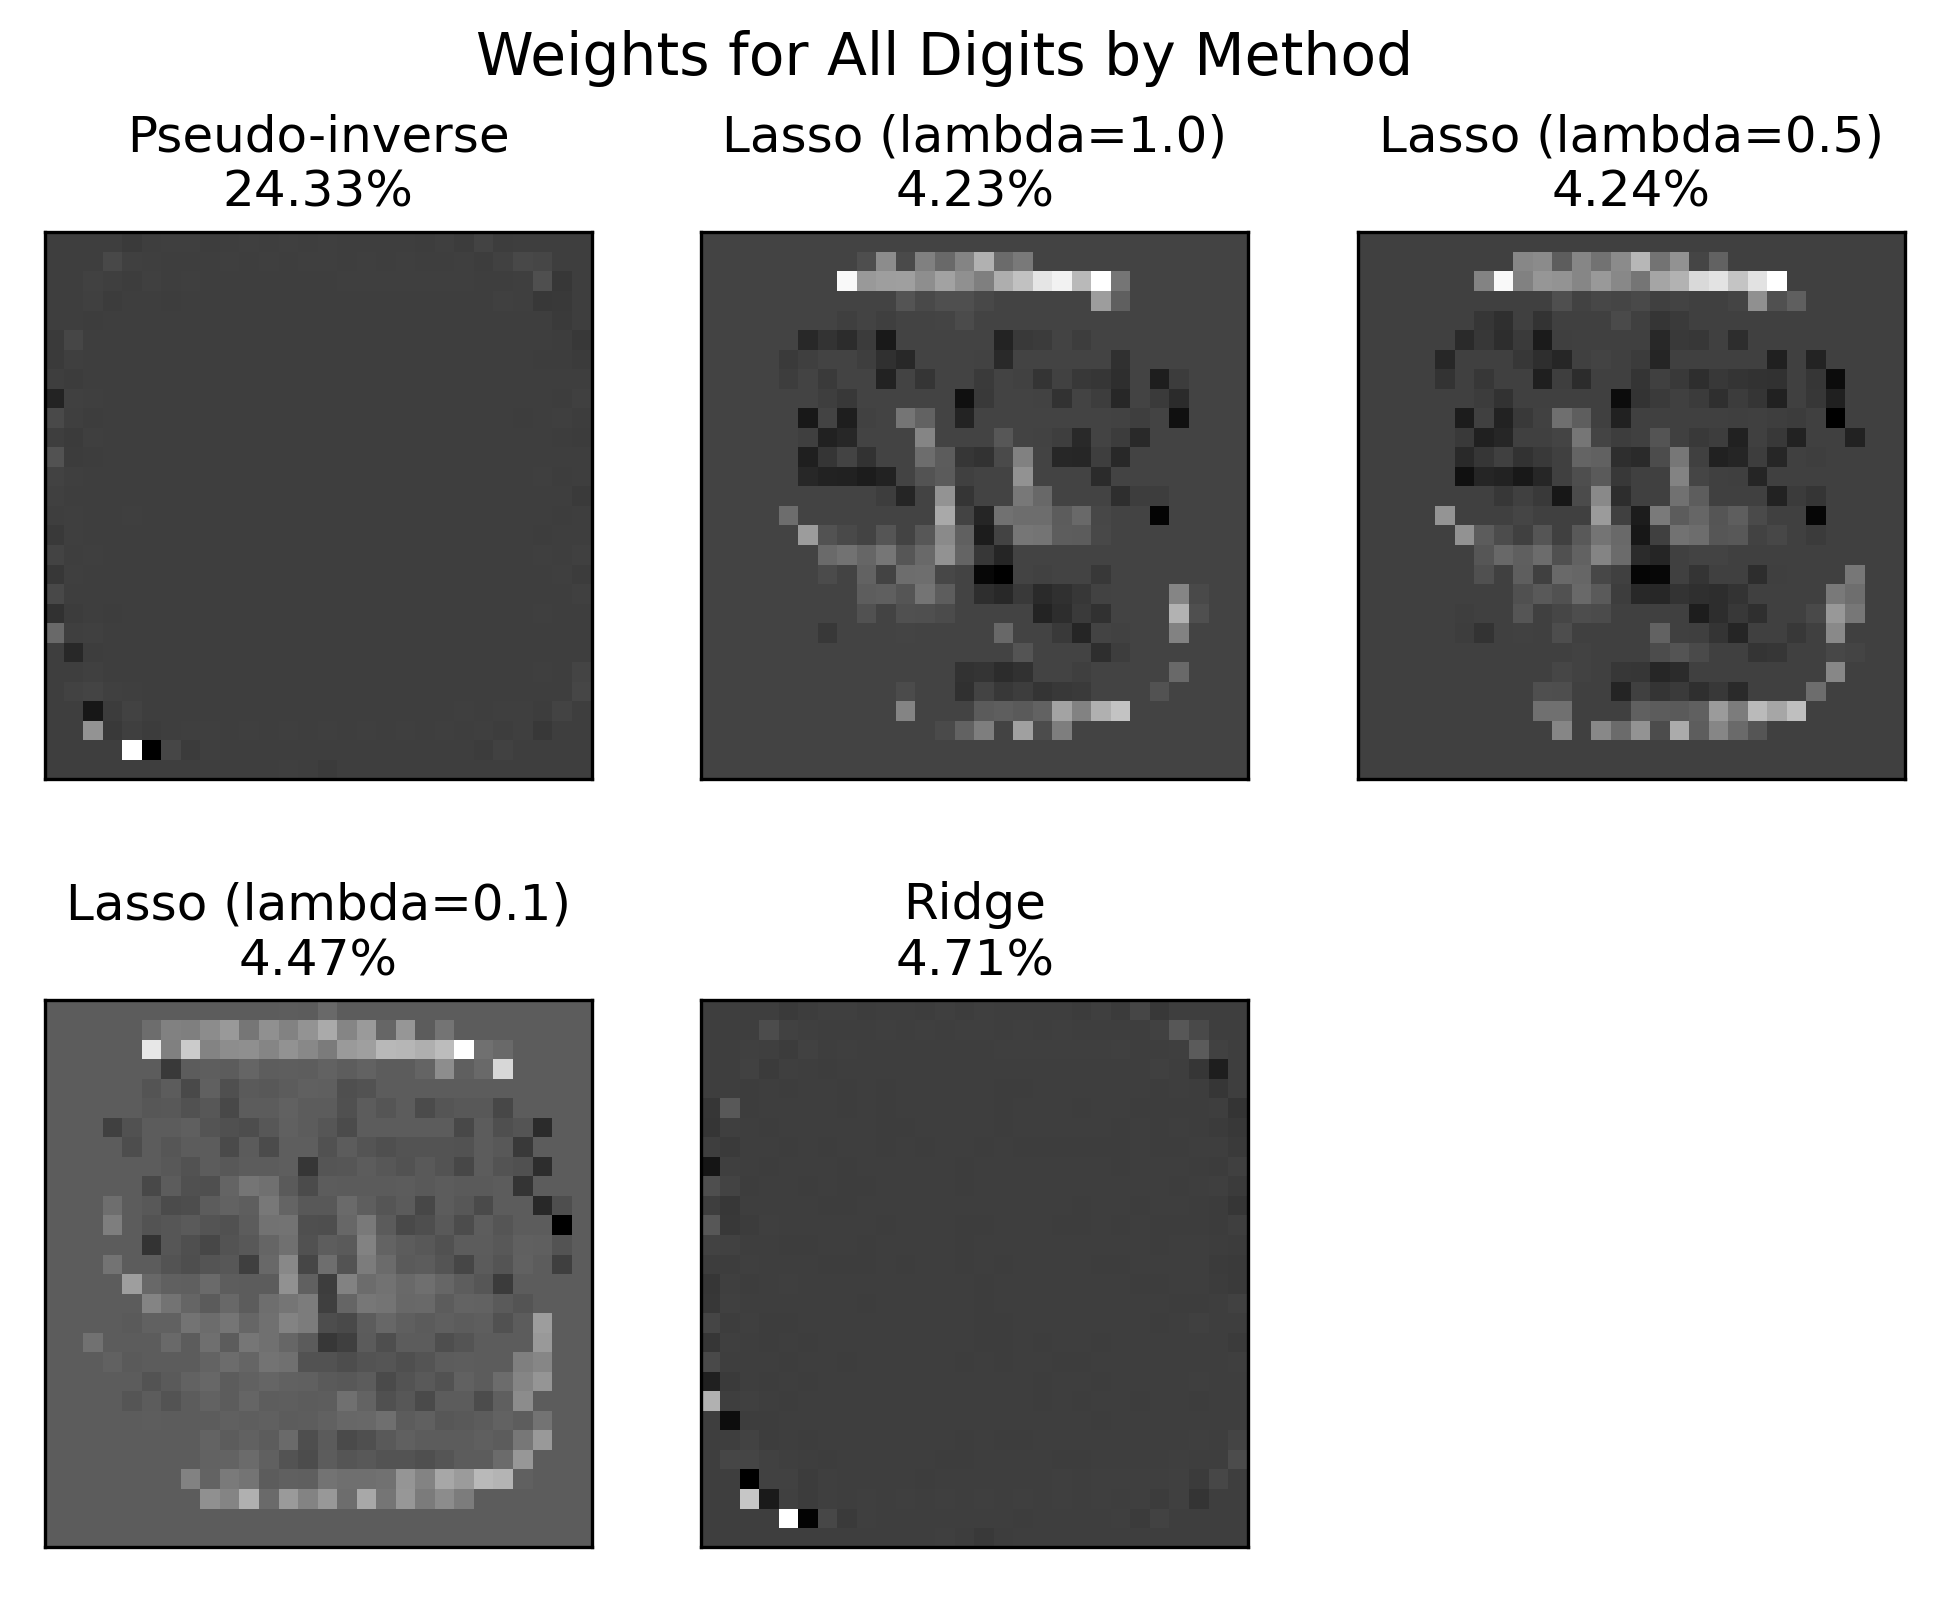
\includegraphics[scale=0.75]{figures/weights_matrix_accuracy_all_digits_all_methods.png}}
\caption{Caption....}
\label{fig1}
\end{figure}

\begin{figure}[ht]
\centerline{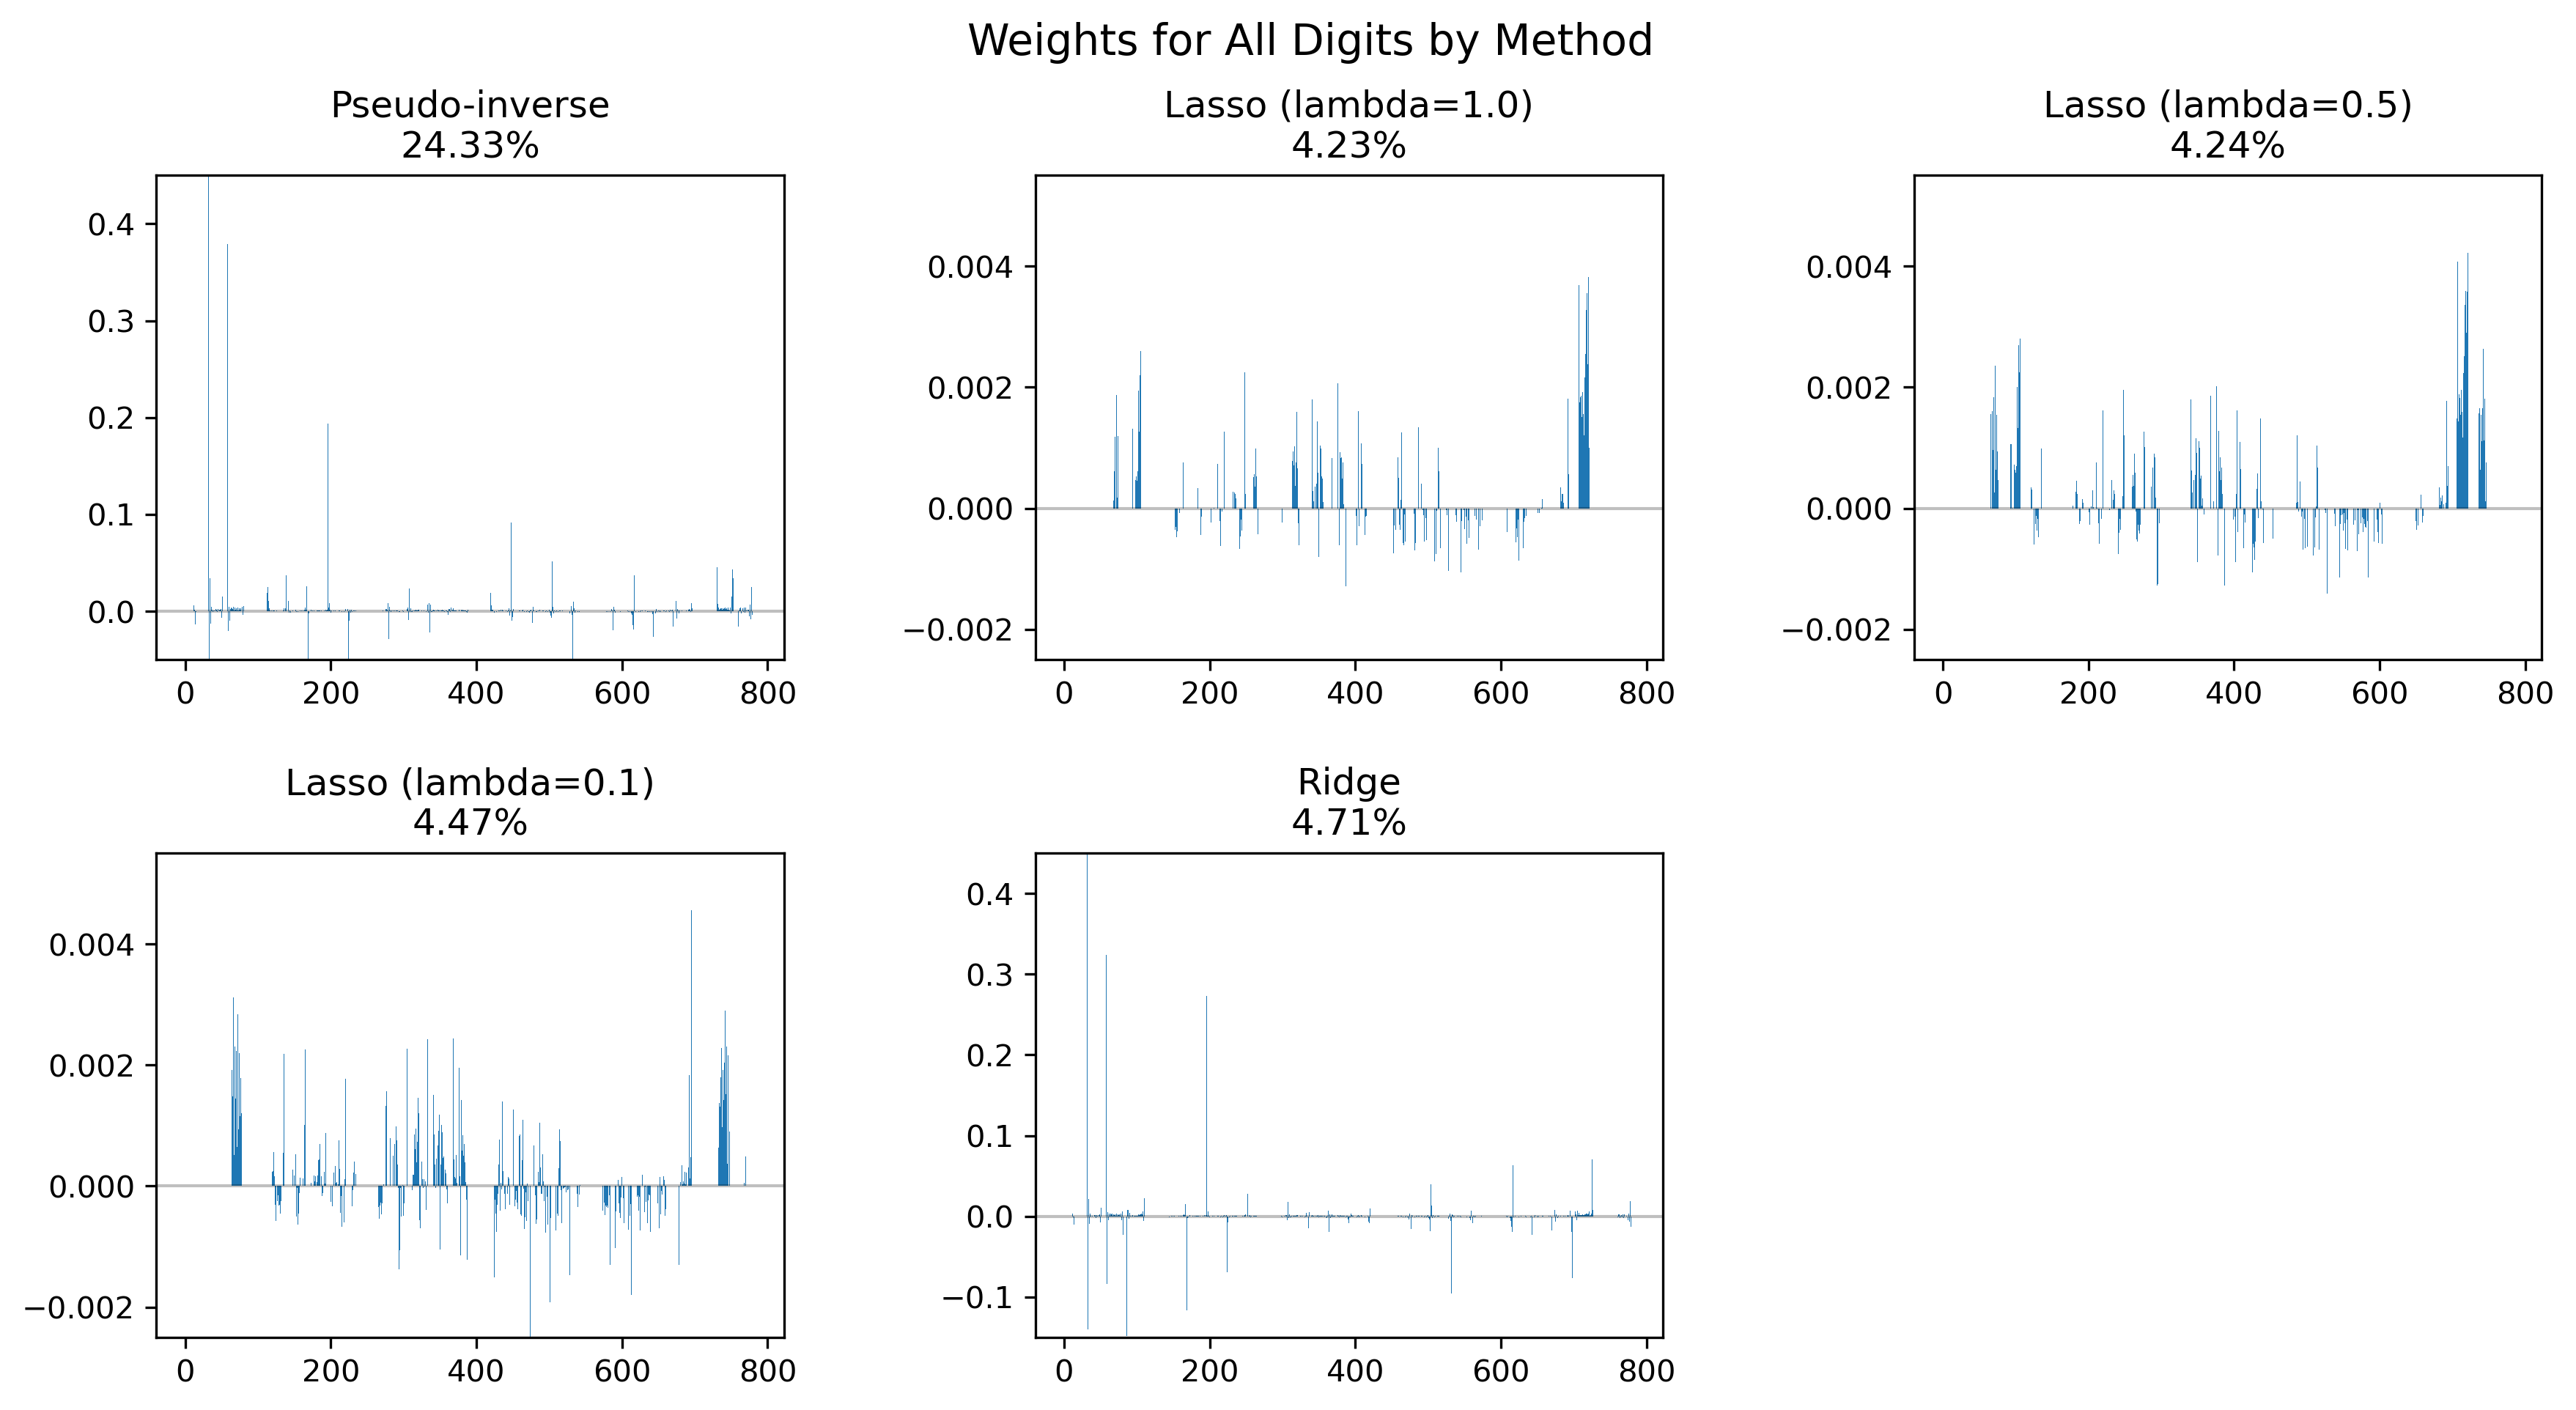
\includegraphics[scale=0.5]{figures/bar_plot_loadings_all_digits_all_methods.png}}
\caption{Caption....}
\label{fig2}
\end{figure}

\begin{figure}[ht]
\centerline{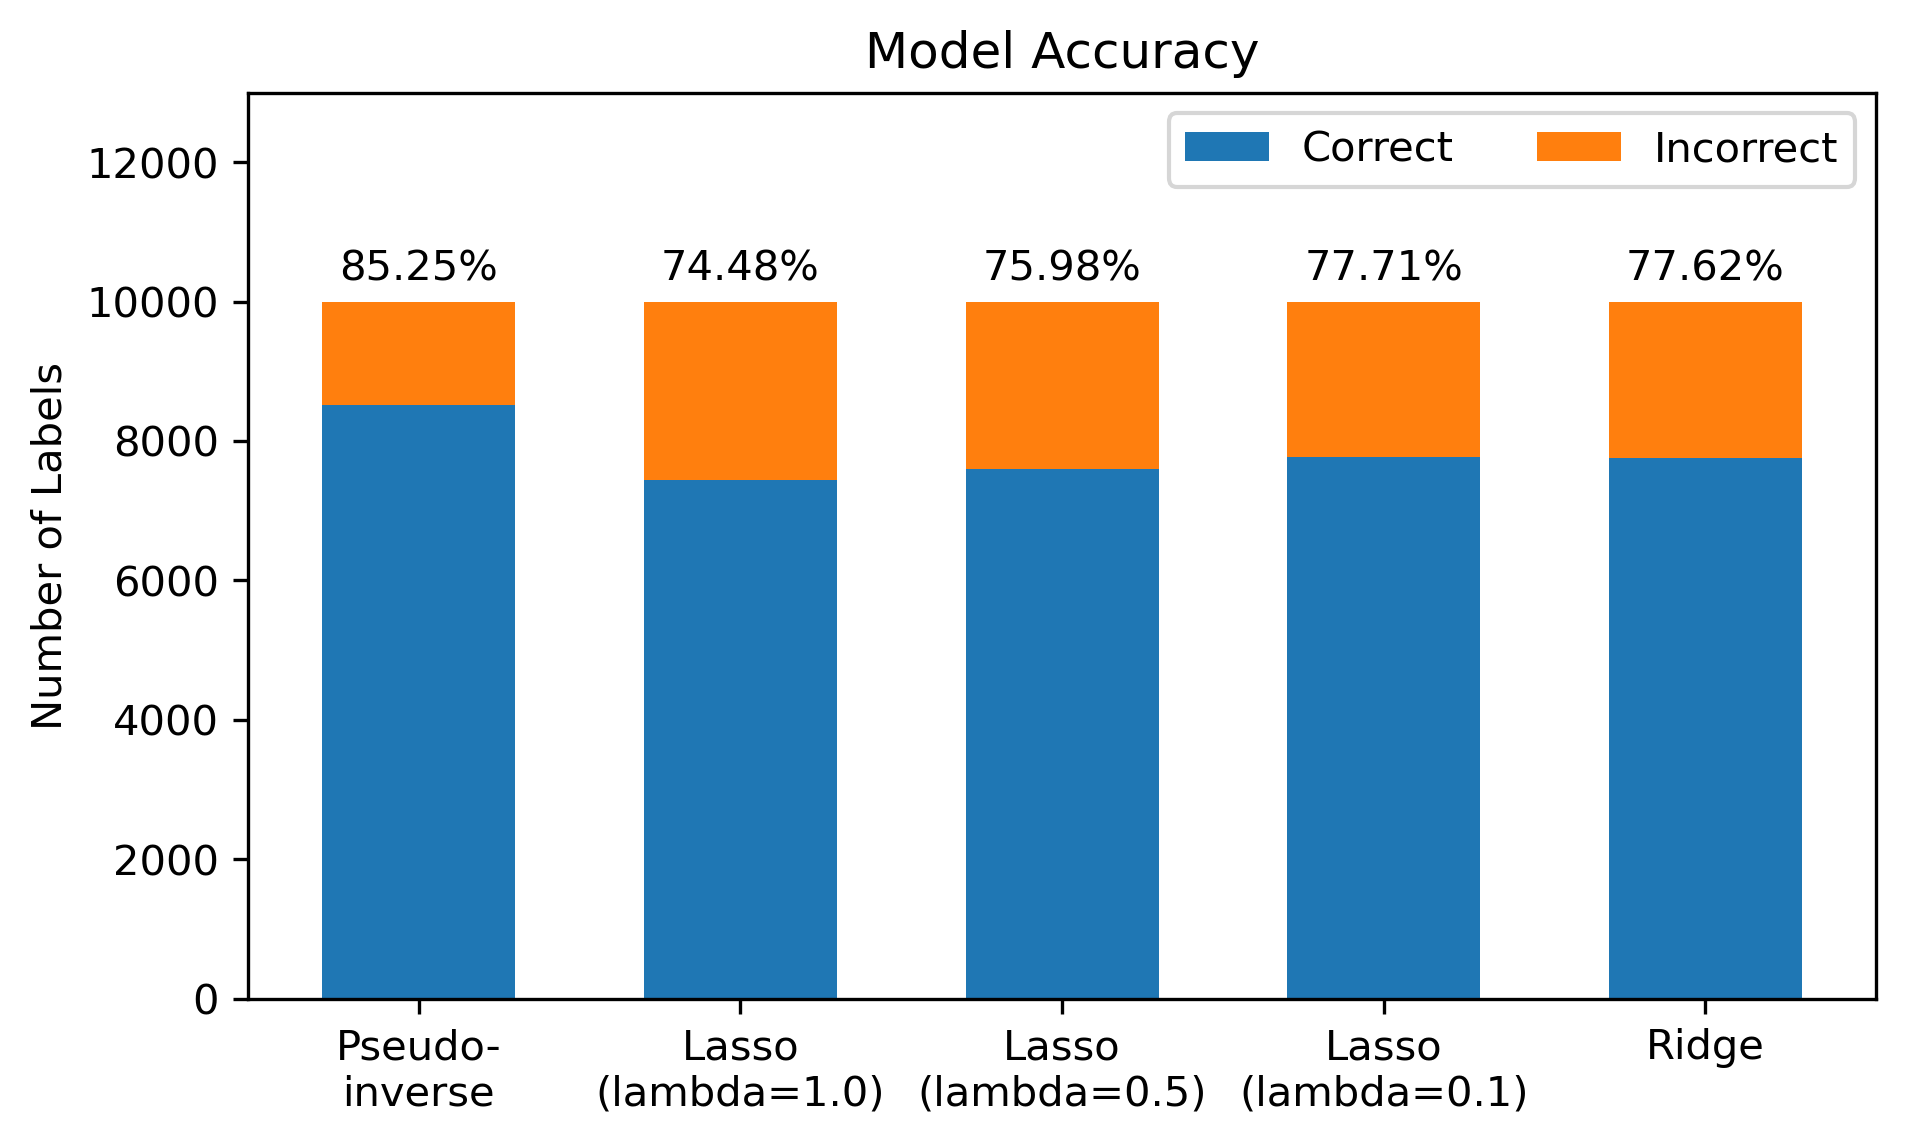
\includegraphics[scale=0.75]{figures/all_data_accuracy_comparison.png}}
\caption{Caption....}
\label{fig3}
\end{figure}

\begin{figure}[ht]
\centerline{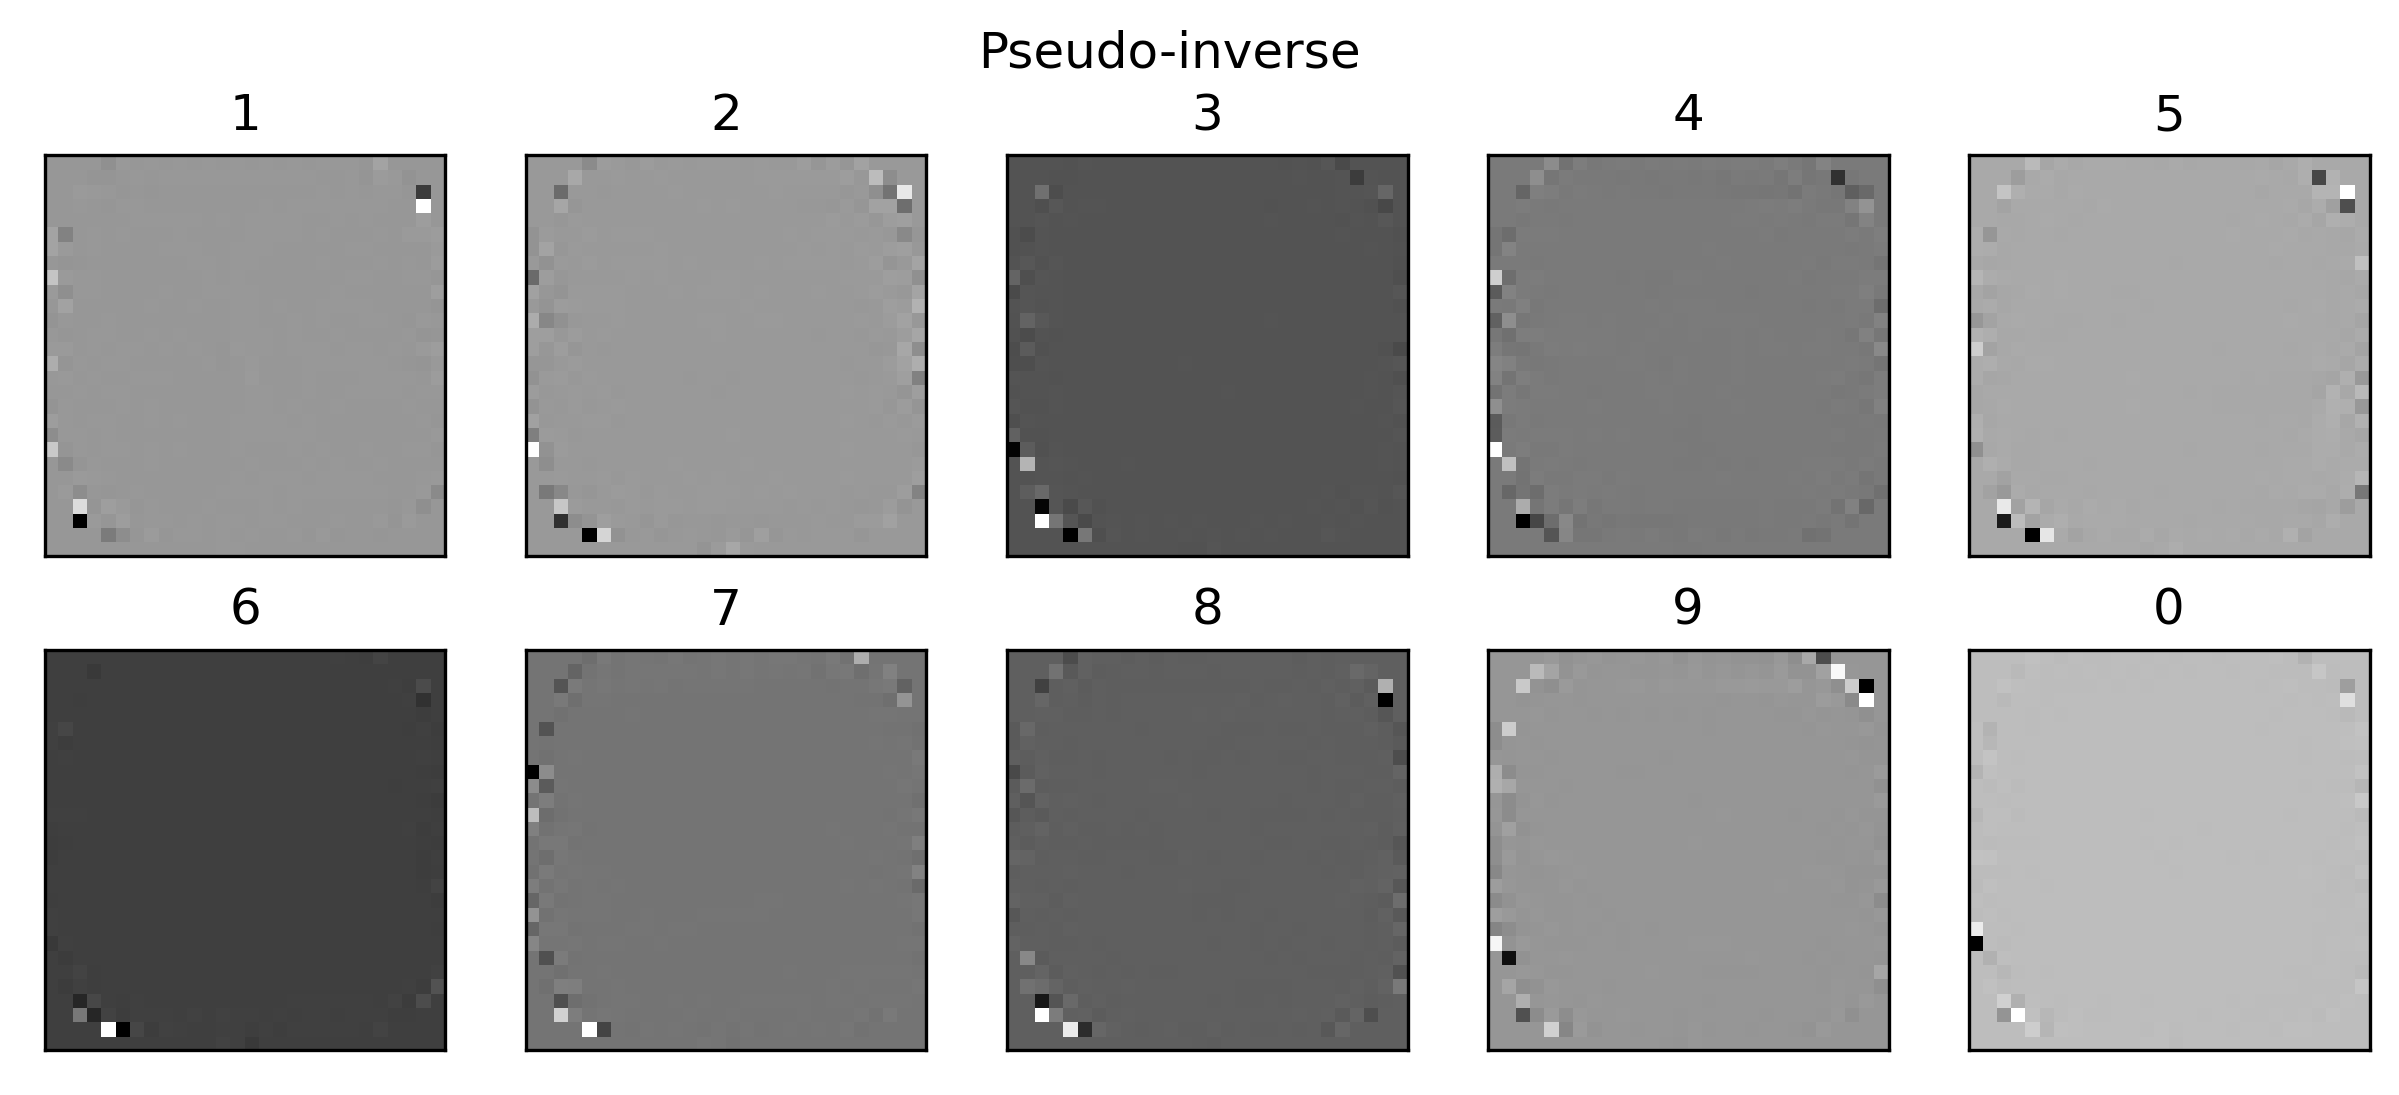
\includegraphics[scale=0.8]{figures/weight_matrix_pinv.png}}
\label{fig4a}
\end{figure}

\begin{figure}[ht]
\centerline{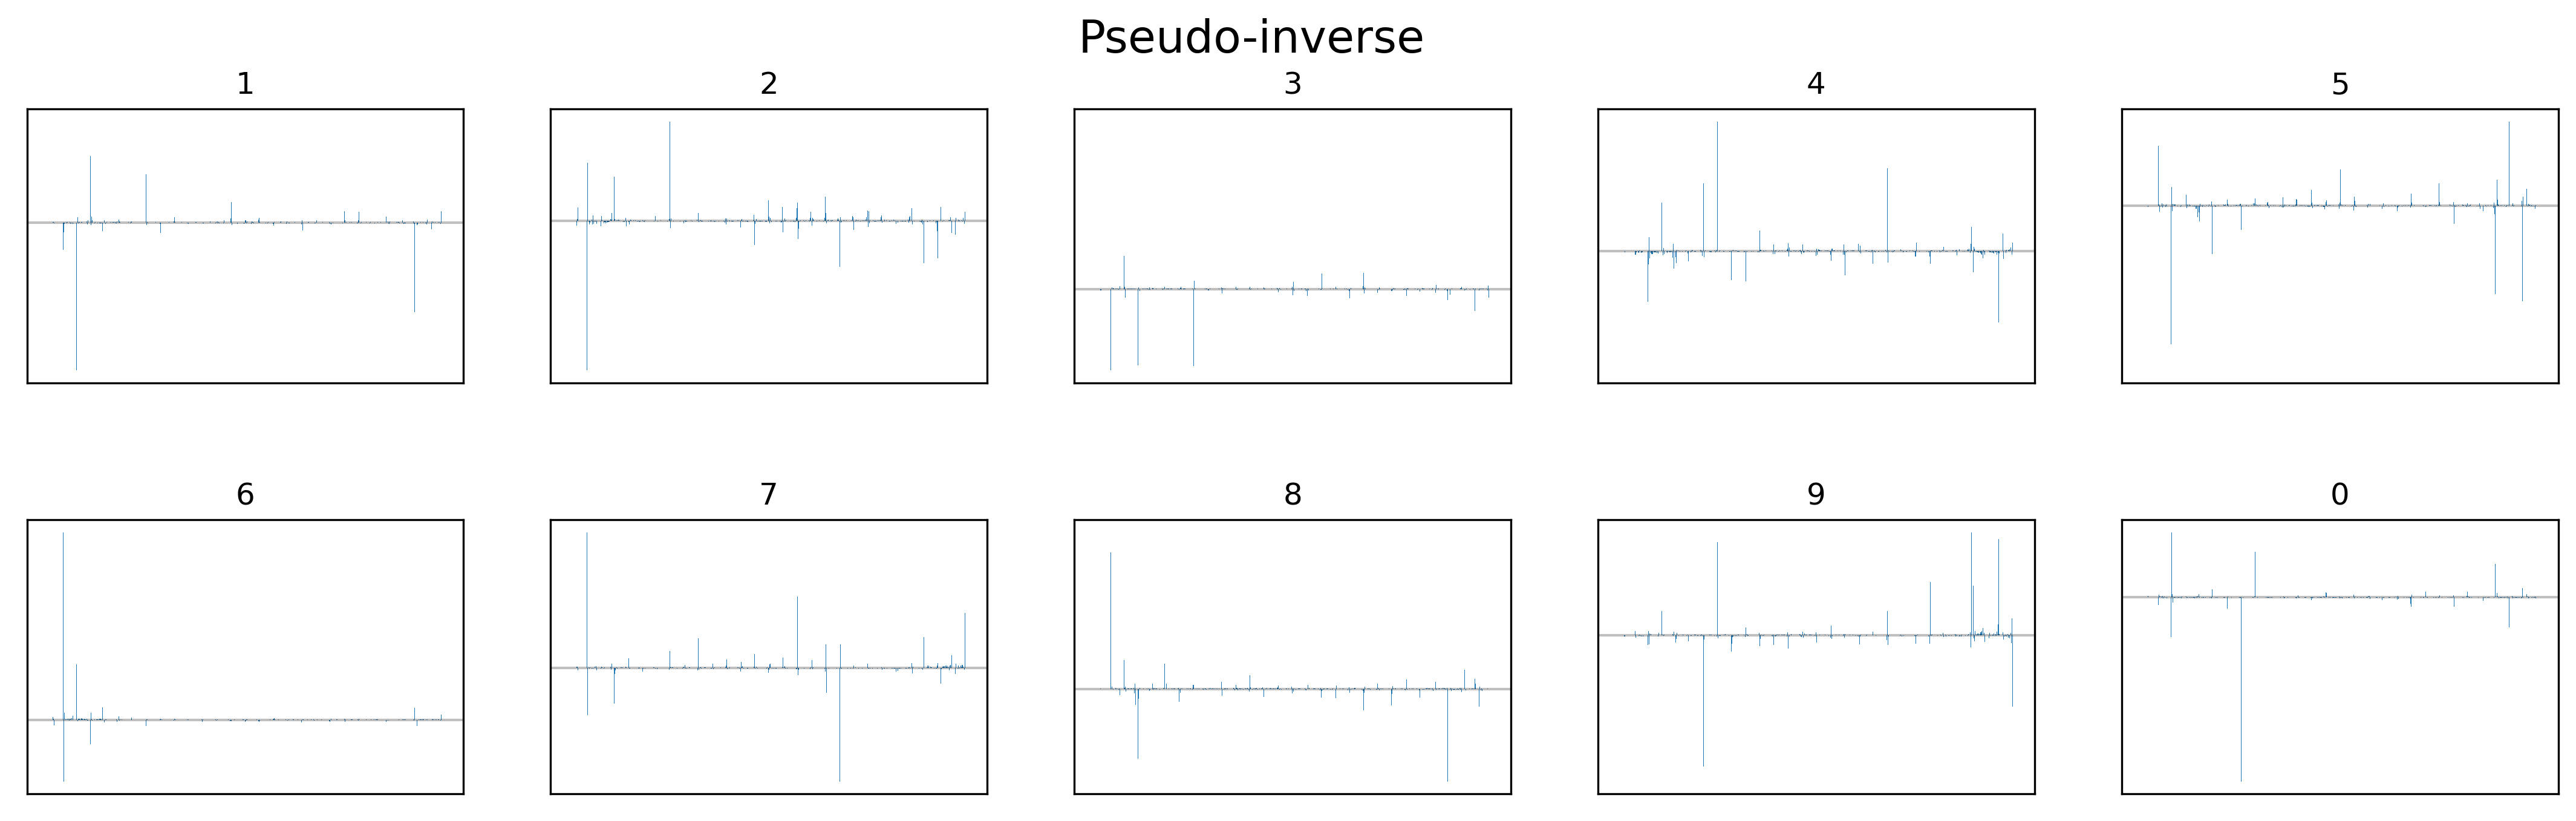
\includegraphics[scale=0.5]{figures/bar_plot_loadings_pinv.png}}
\caption{Caption....}
\label{fig4b}
\end{figure}

\begin{figure}[ht]
\centerline{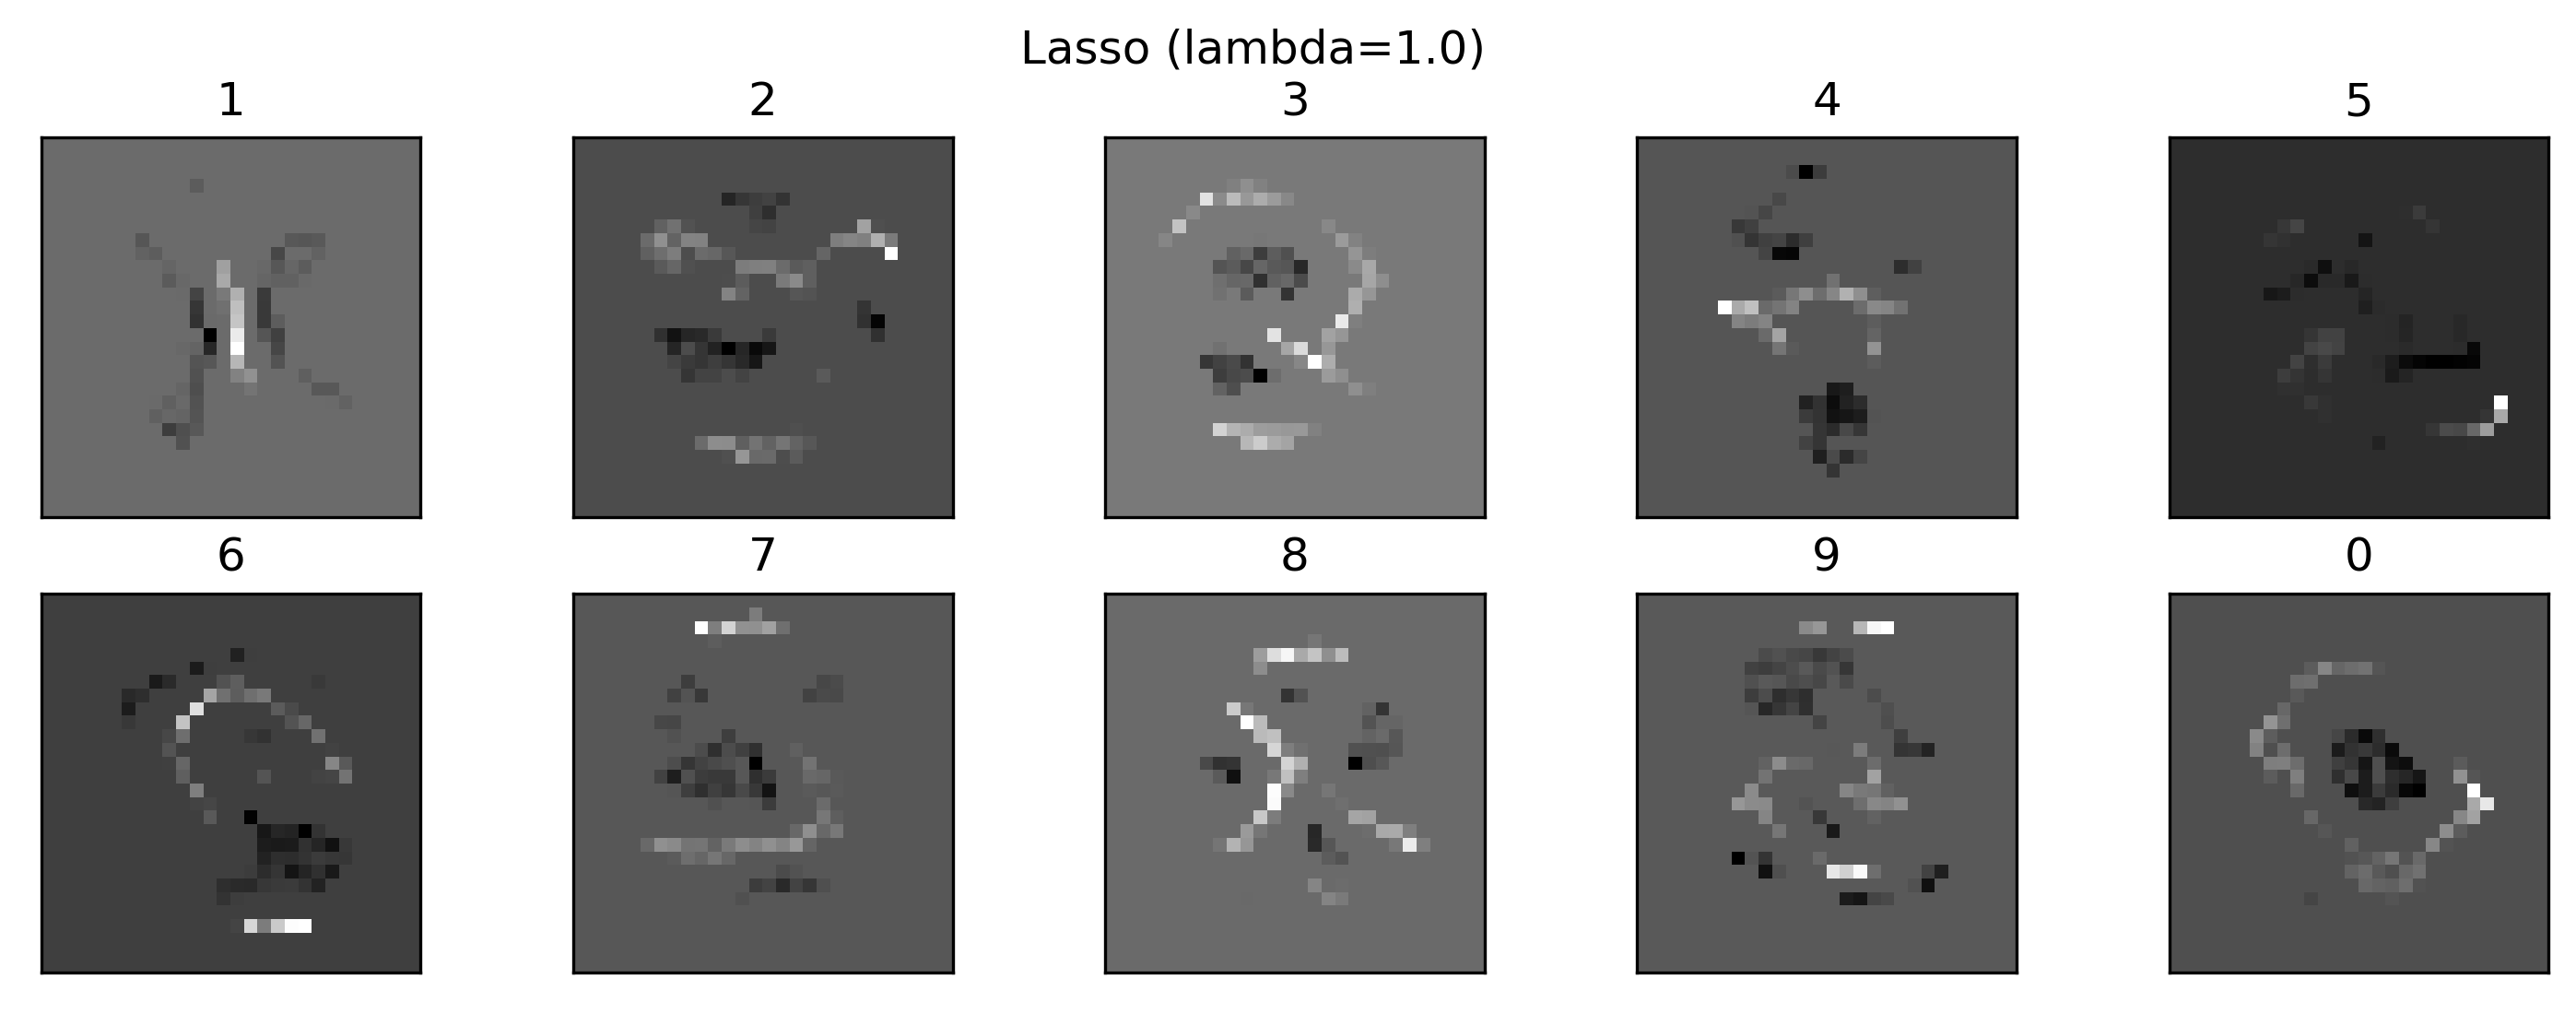
\includegraphics[scale=0.8]{figures/weight_matrix_lasso_1.png}}
\label{fig5a}
\end{figure}

\begin{figure}[ht]
\centerline{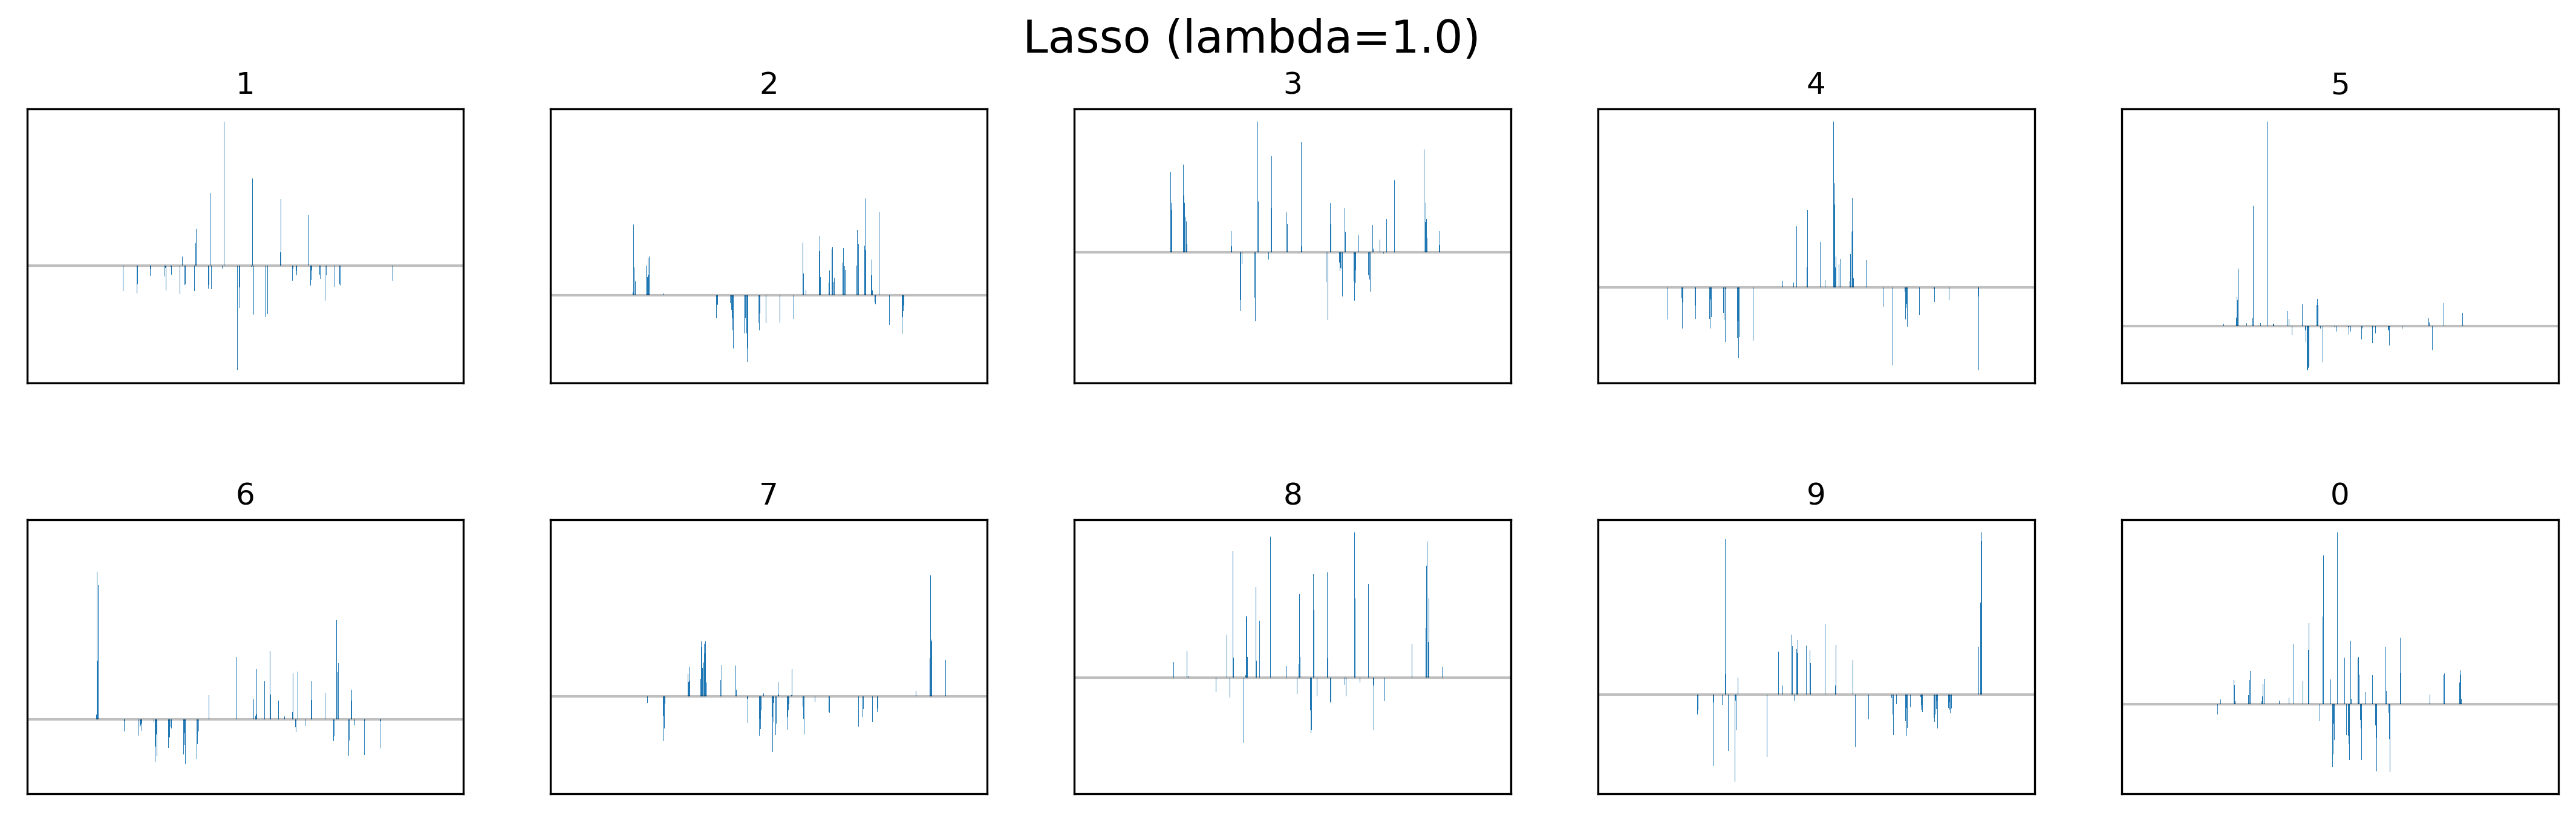
\includegraphics[scale=0.5]{figures/bar_plot_loadings_lasso_1.png}}
\caption{Caption....}
\label{fig5b}
\end{figure}

\begin{figure}[ht]
\centerline{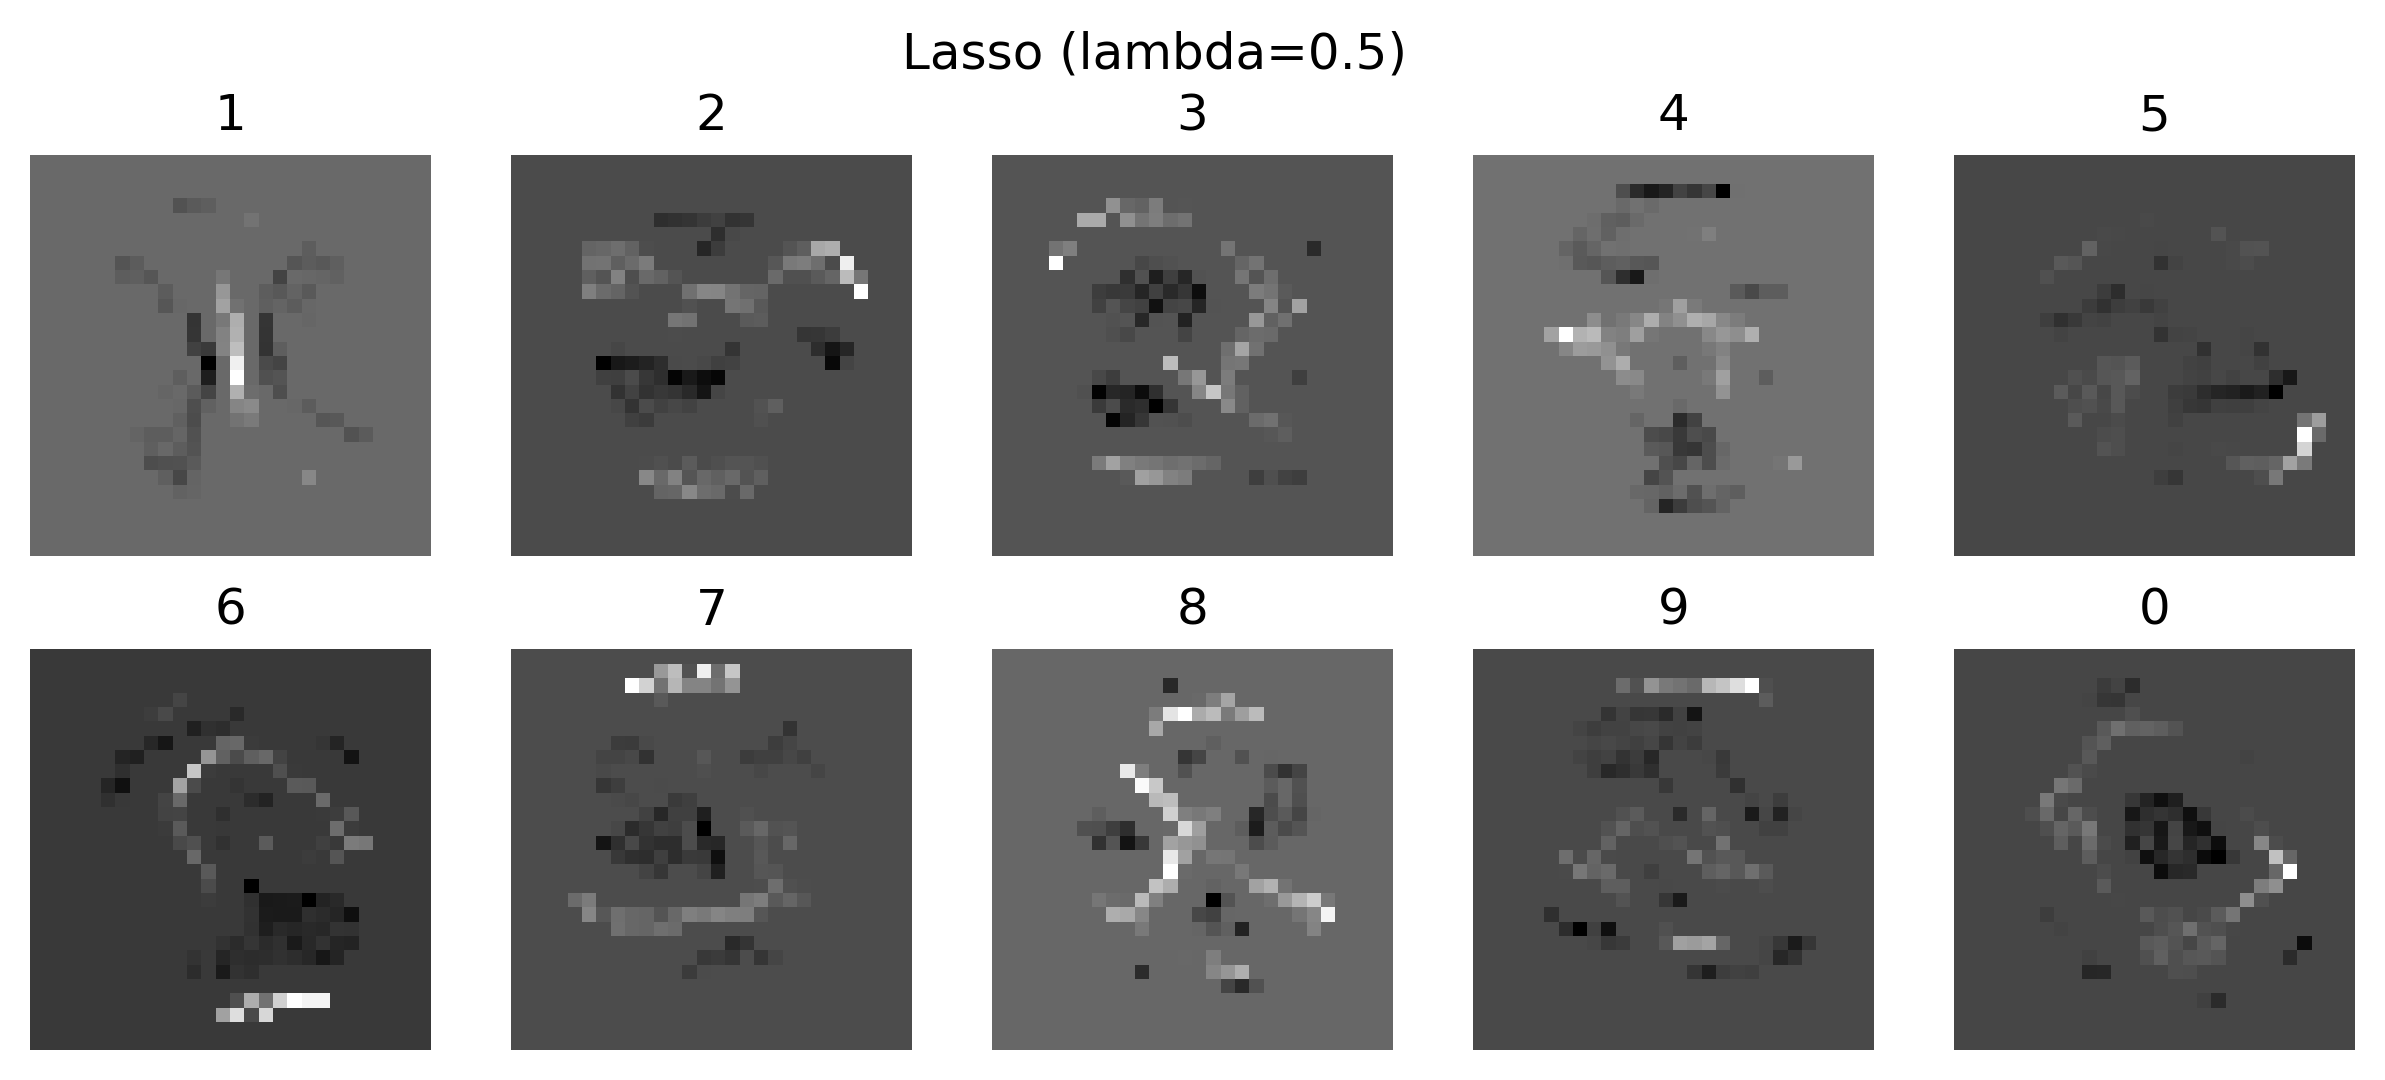
\includegraphics[scale=0.8]{figures/weight_matrix_lasso_05.png}}
\label{fig6a}
\end{figure}

\begin{figure}[ht]
\centerline{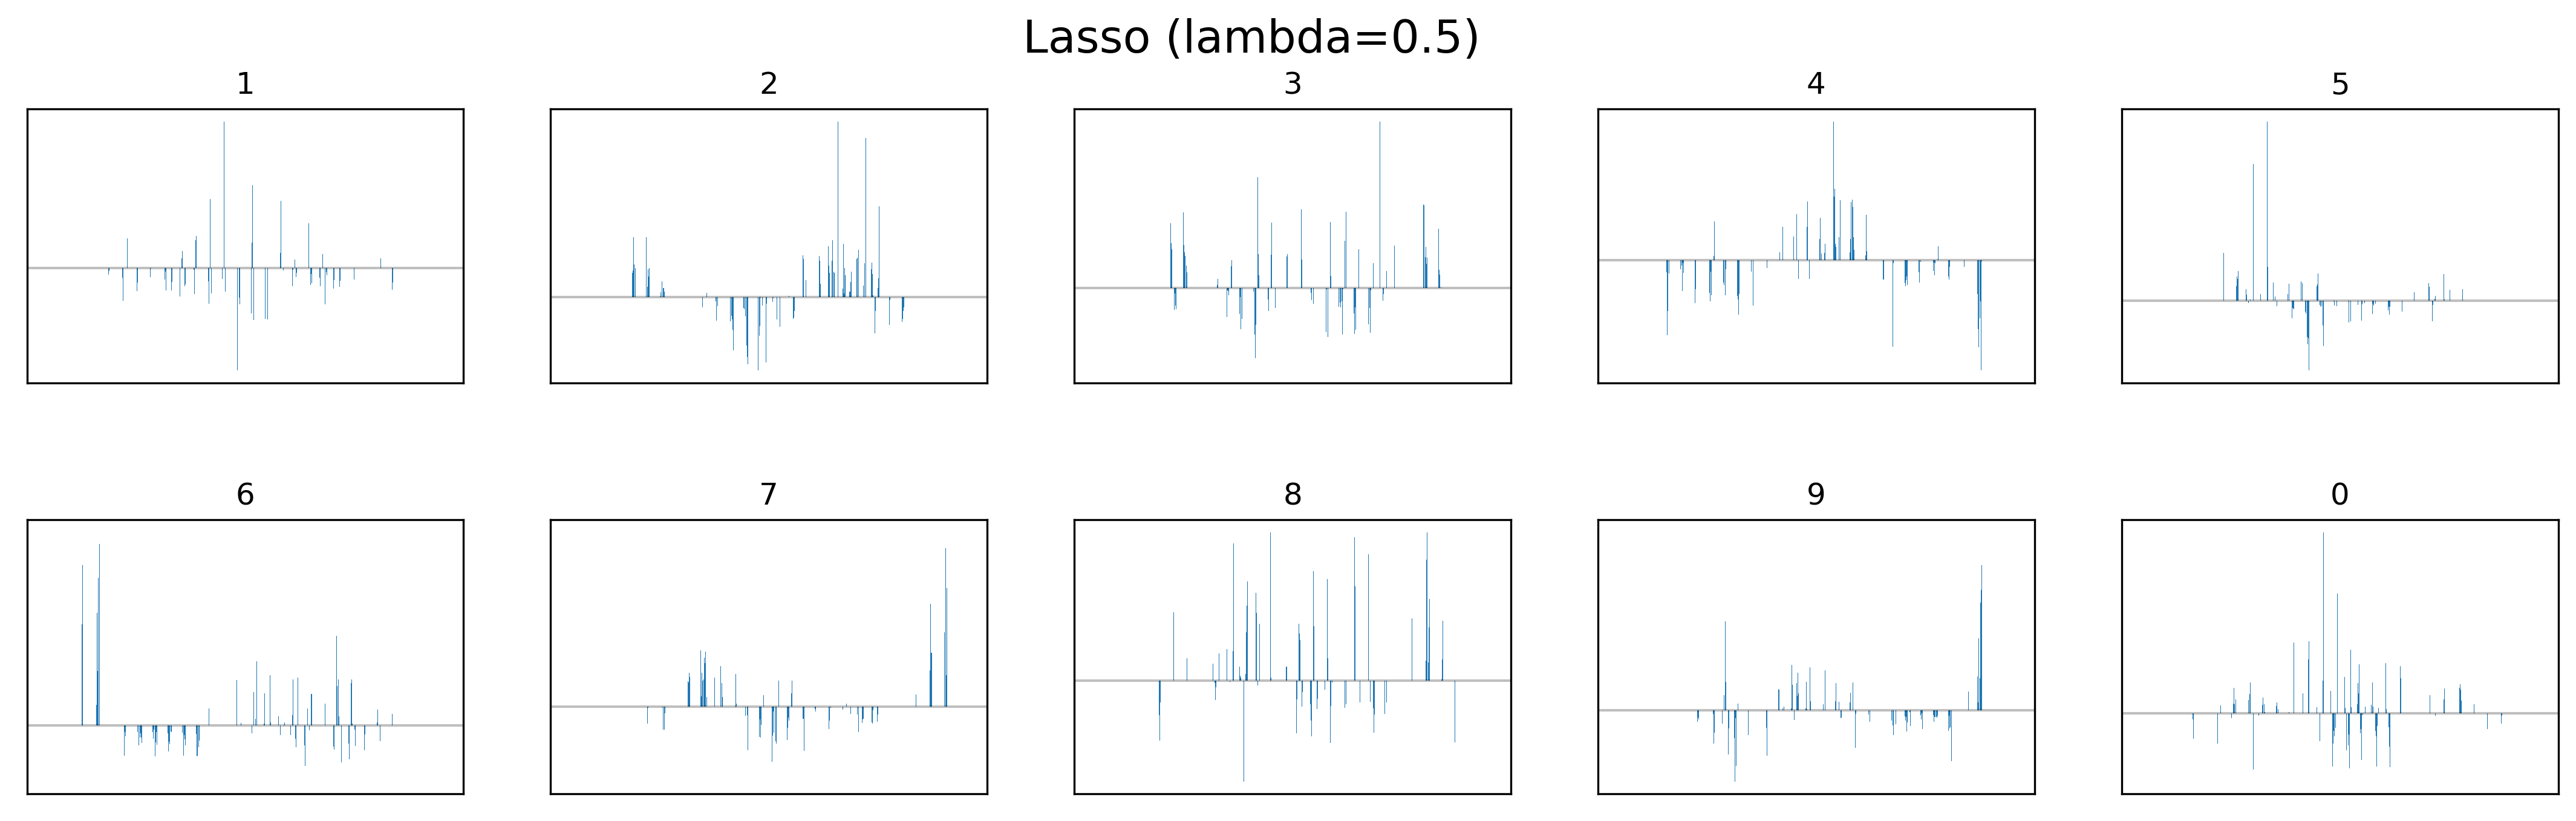
\includegraphics[scale=0.5]{figures/bar_plot_loadings_lasso_05.png}}
\caption{Caption....}
\label{fig6b}
\end{figure}

\begin{figure}[ht]
\centerline{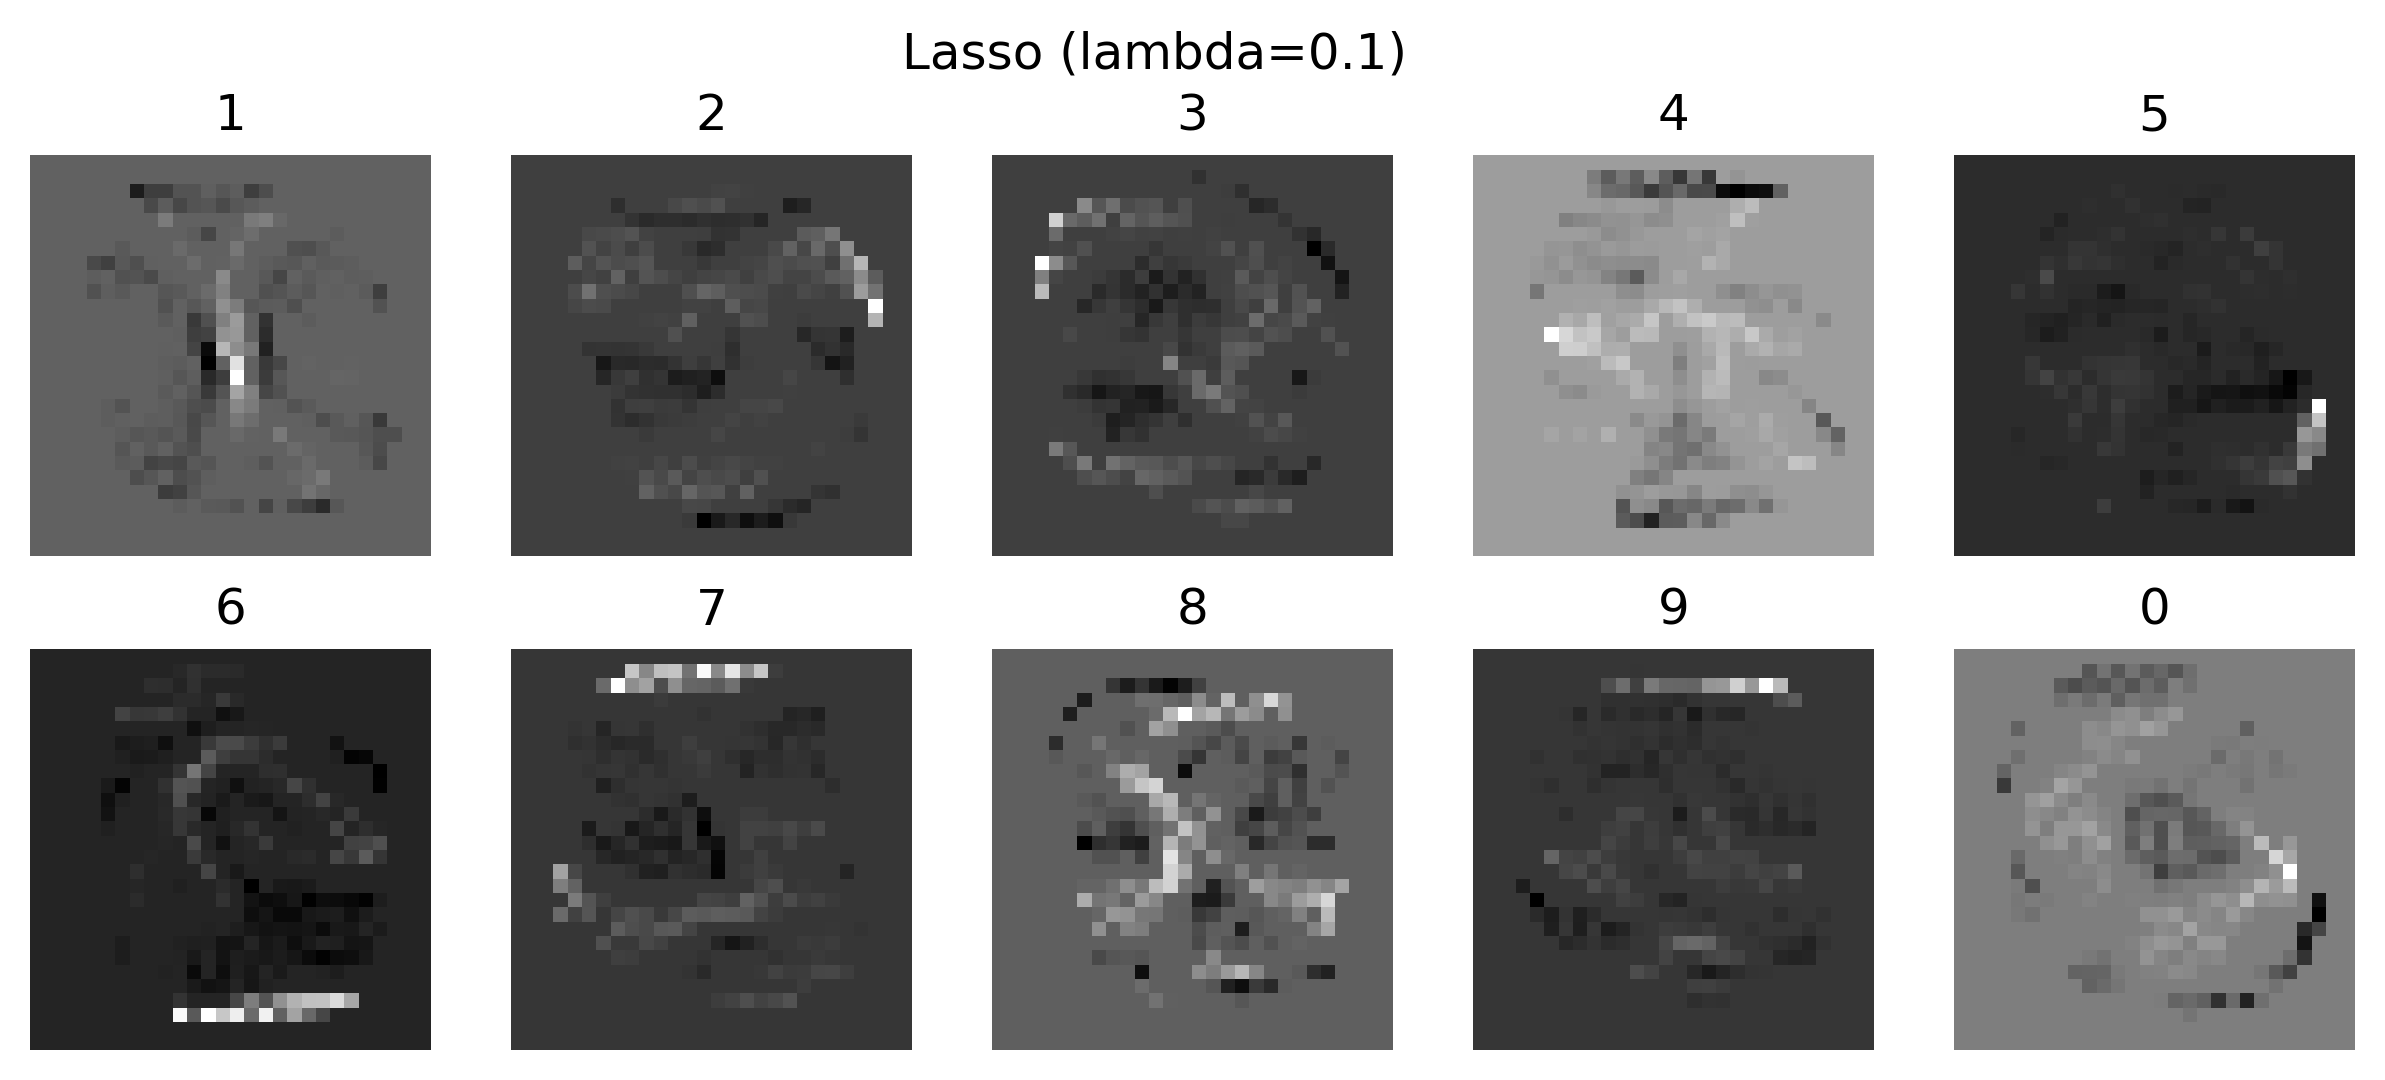
\includegraphics[scale=0.8]{figures/weight_matrix_lasso_01.png}}
\label{fig7a}
\end{figure}

\begin{figure}[ht]
\centerline{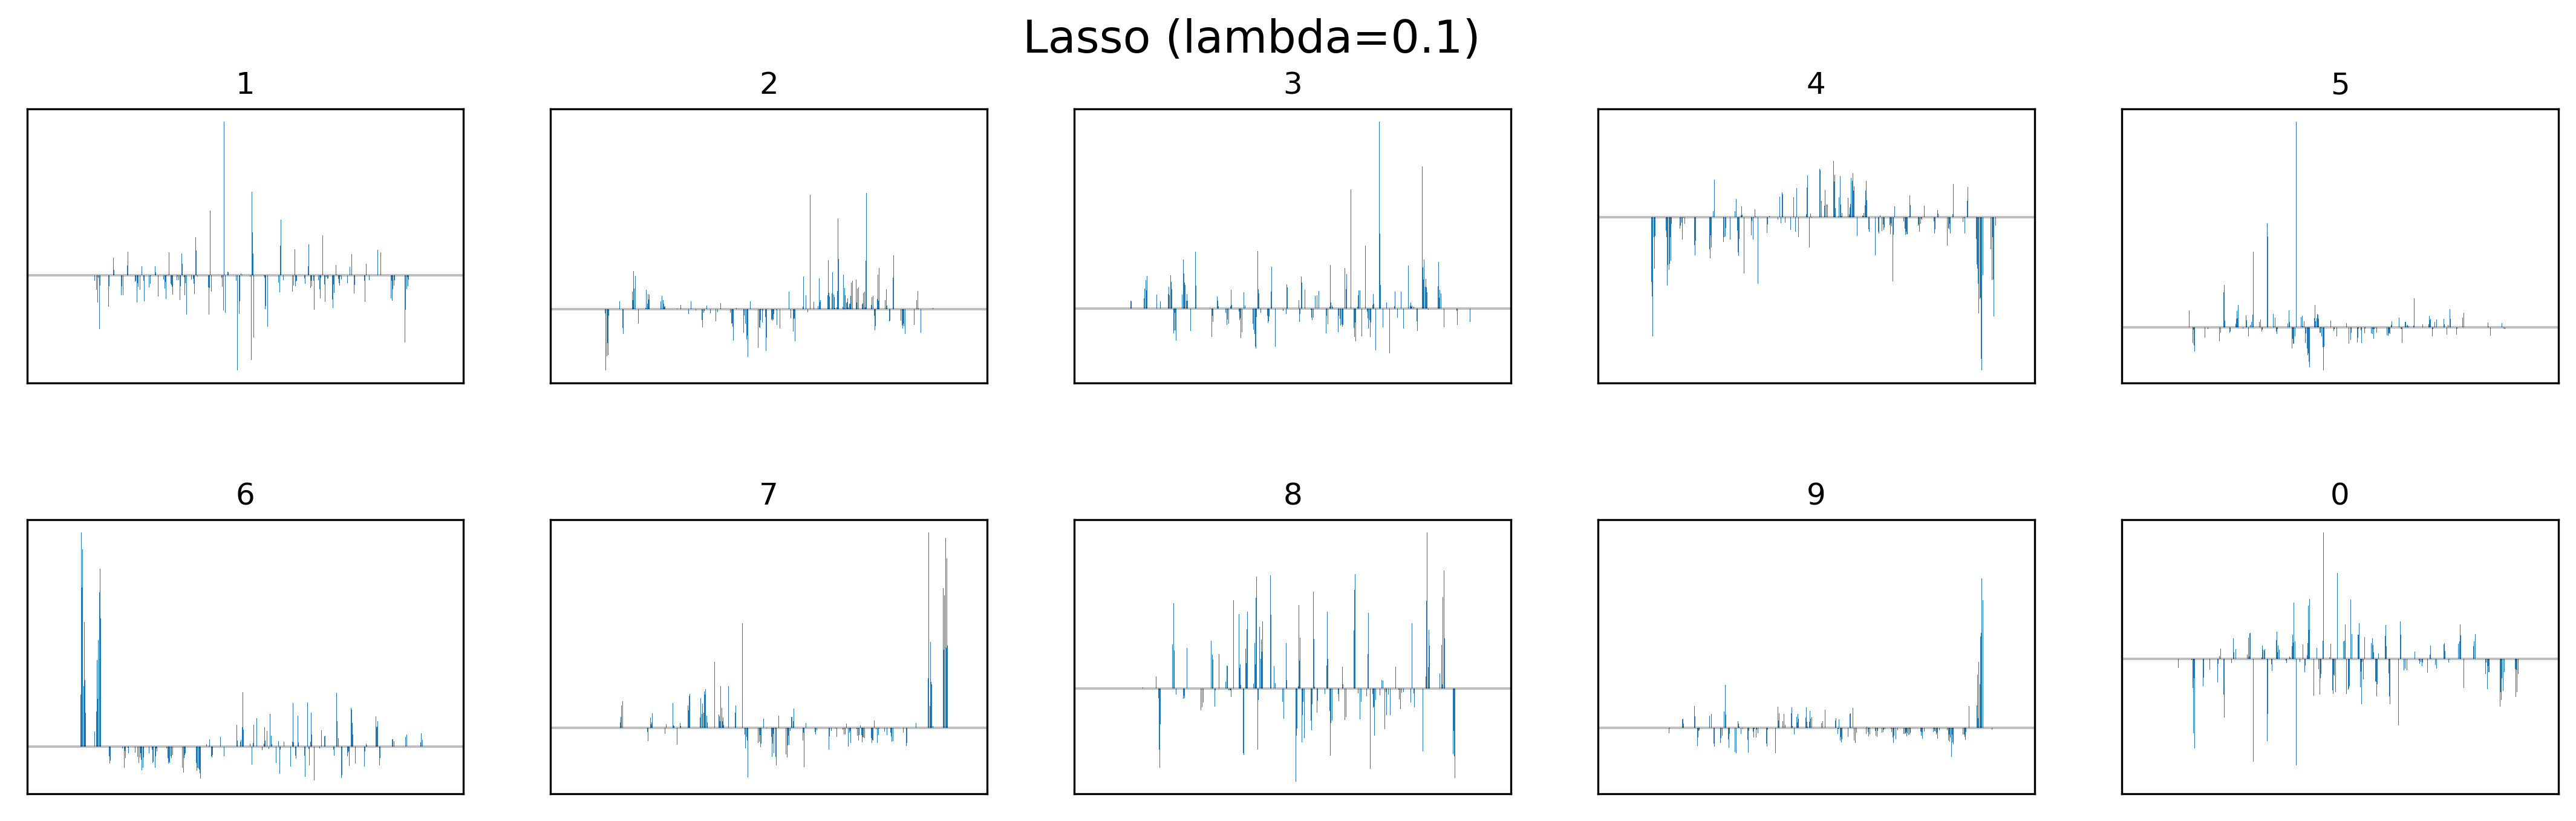
\includegraphics[scale=0.5]{figures/bar_plot_loadings_lasso_01.png}}
\caption{Caption....}
\label{fig7b}
\end{figure}

\begin{figure}[ht]
\centerline{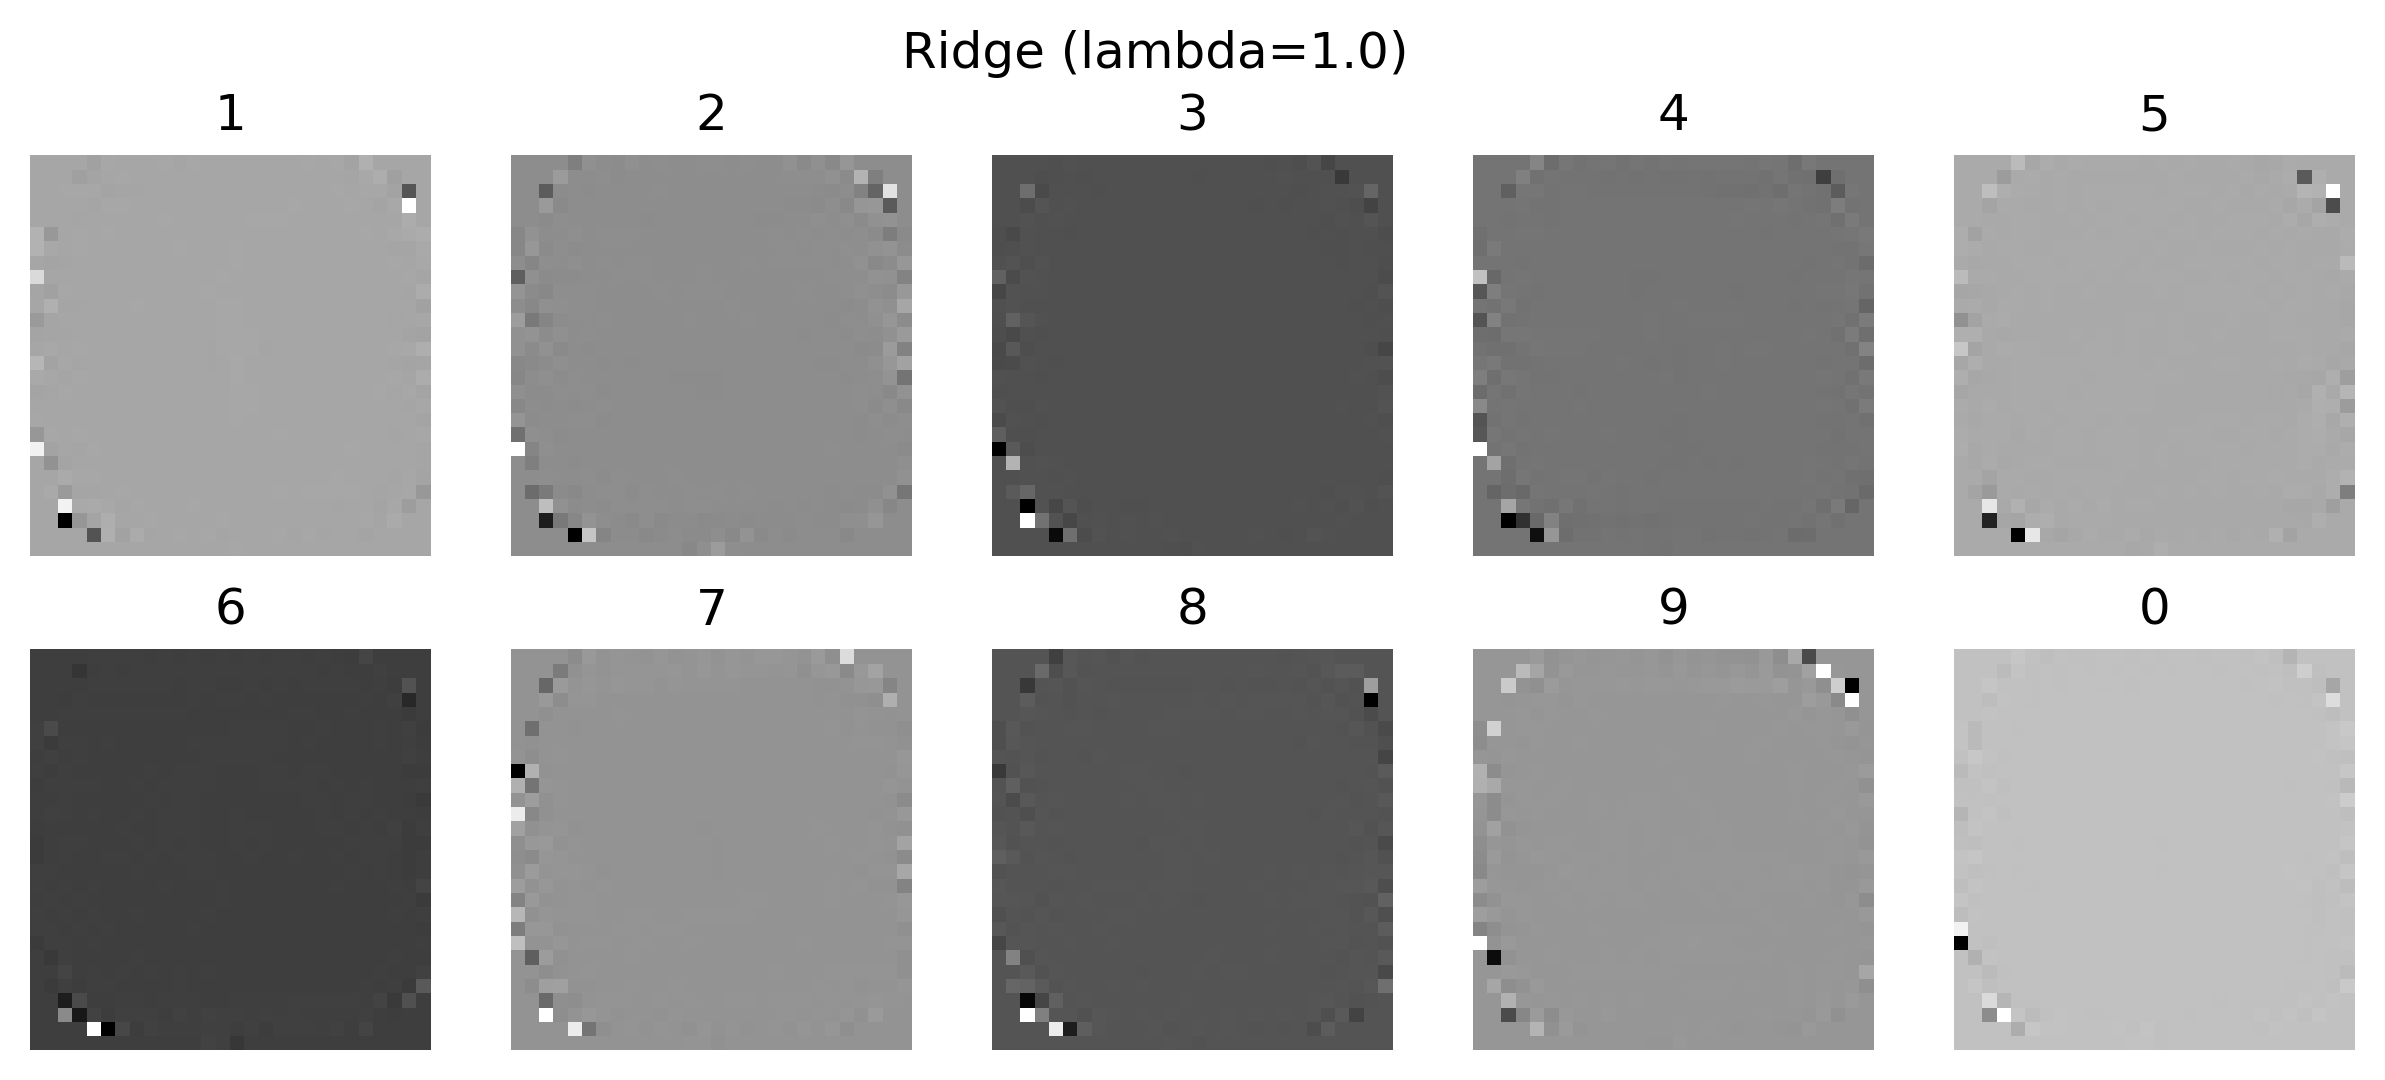
\includegraphics[scale=0.8]{figures/weight_matrix_ridge.png}}
\label{fig8a}
\end{figure}

\begin{figure}[ht]
\centerline{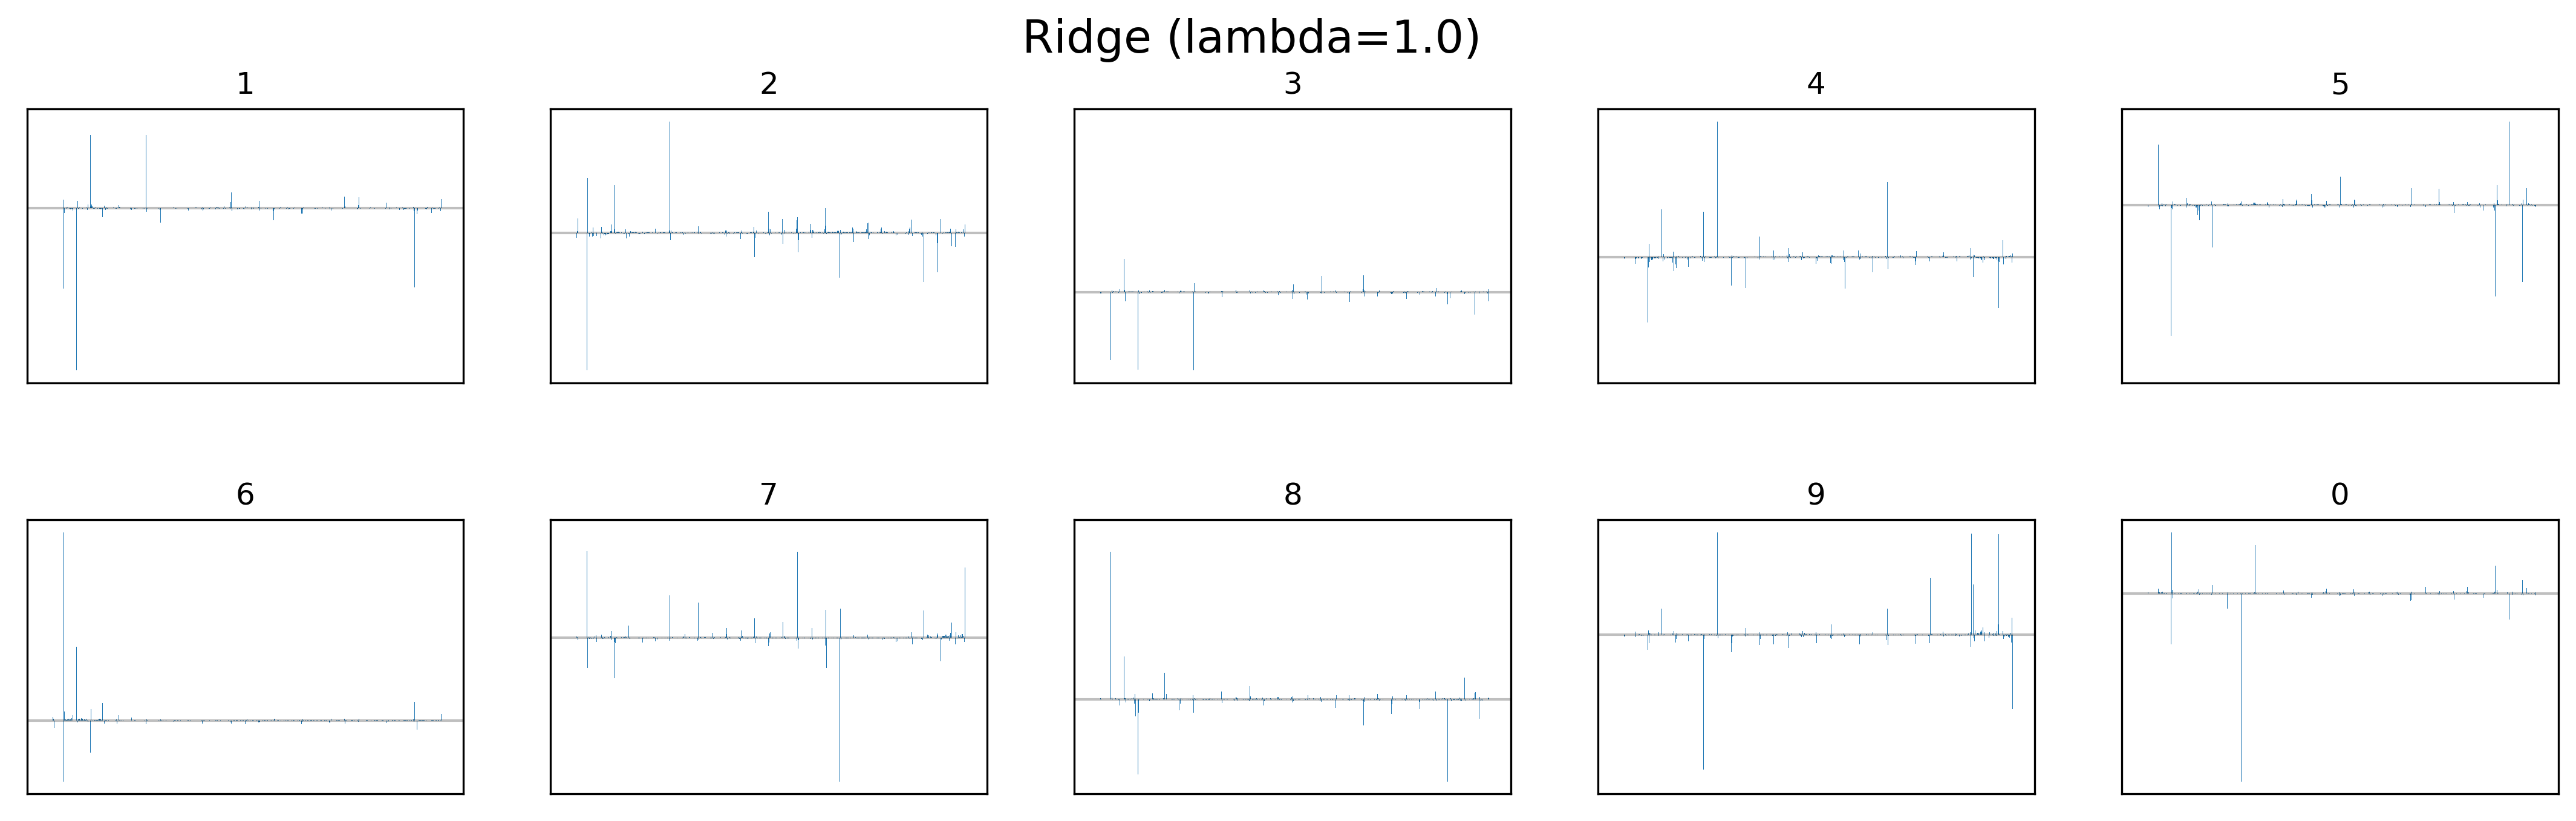
\includegraphics[scale=0.5]{figures/bar_plot_loadings_ridge.png}}
\caption{Caption....}
\label{fig8b}
\end{figure}

\begin{figure}[ht]
\centerline{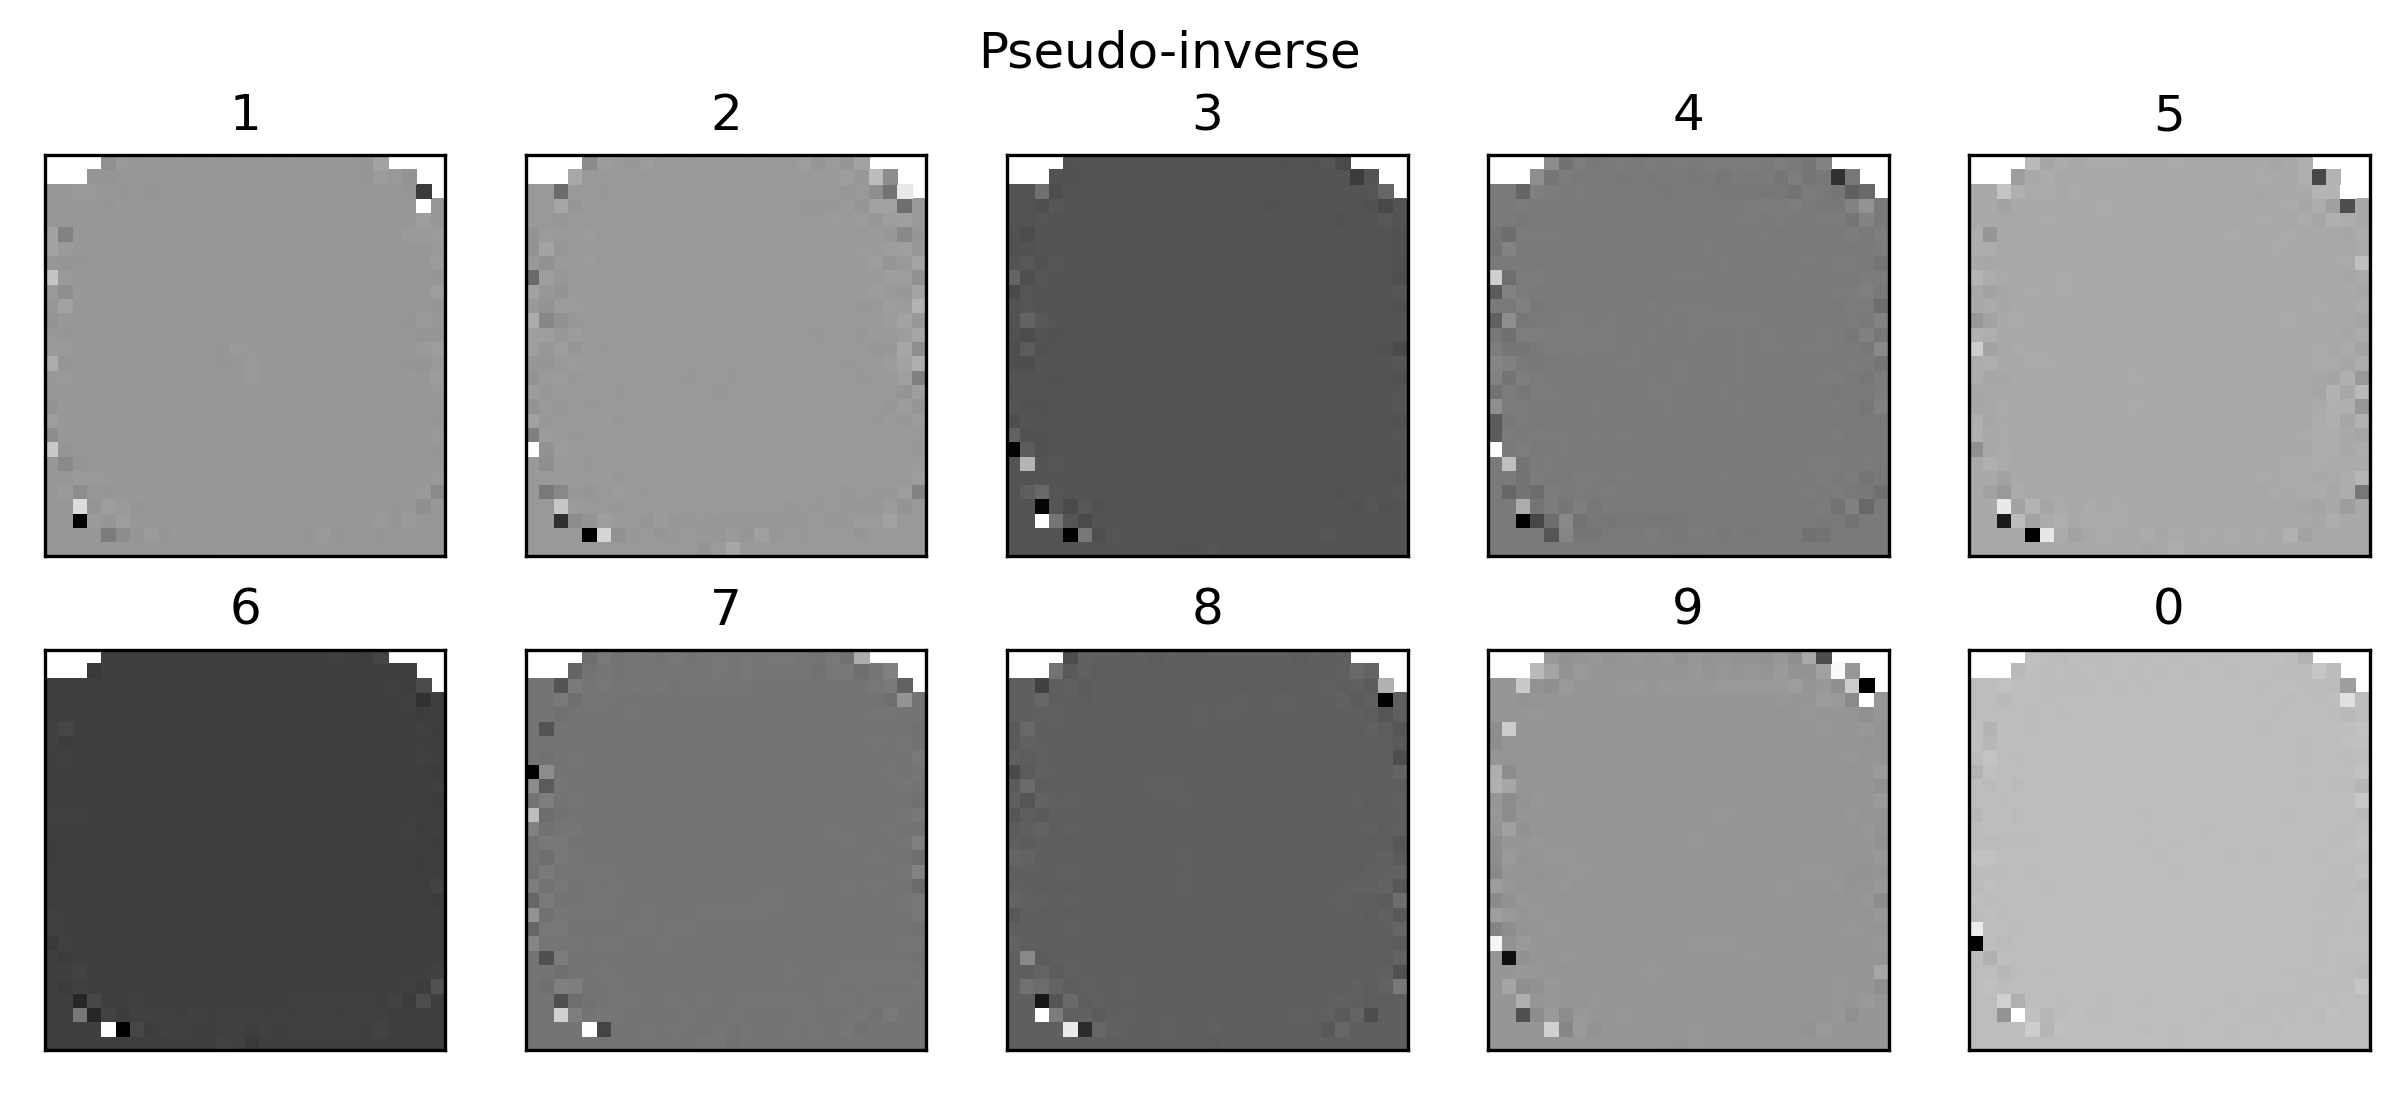
\includegraphics[scale=0.75]{figures/weight_matrix_pinv_no_zeros.png}}
\caption{Caption....}
\label{fig9}
\end{figure}

\begin{figure}[ht]
\centerline{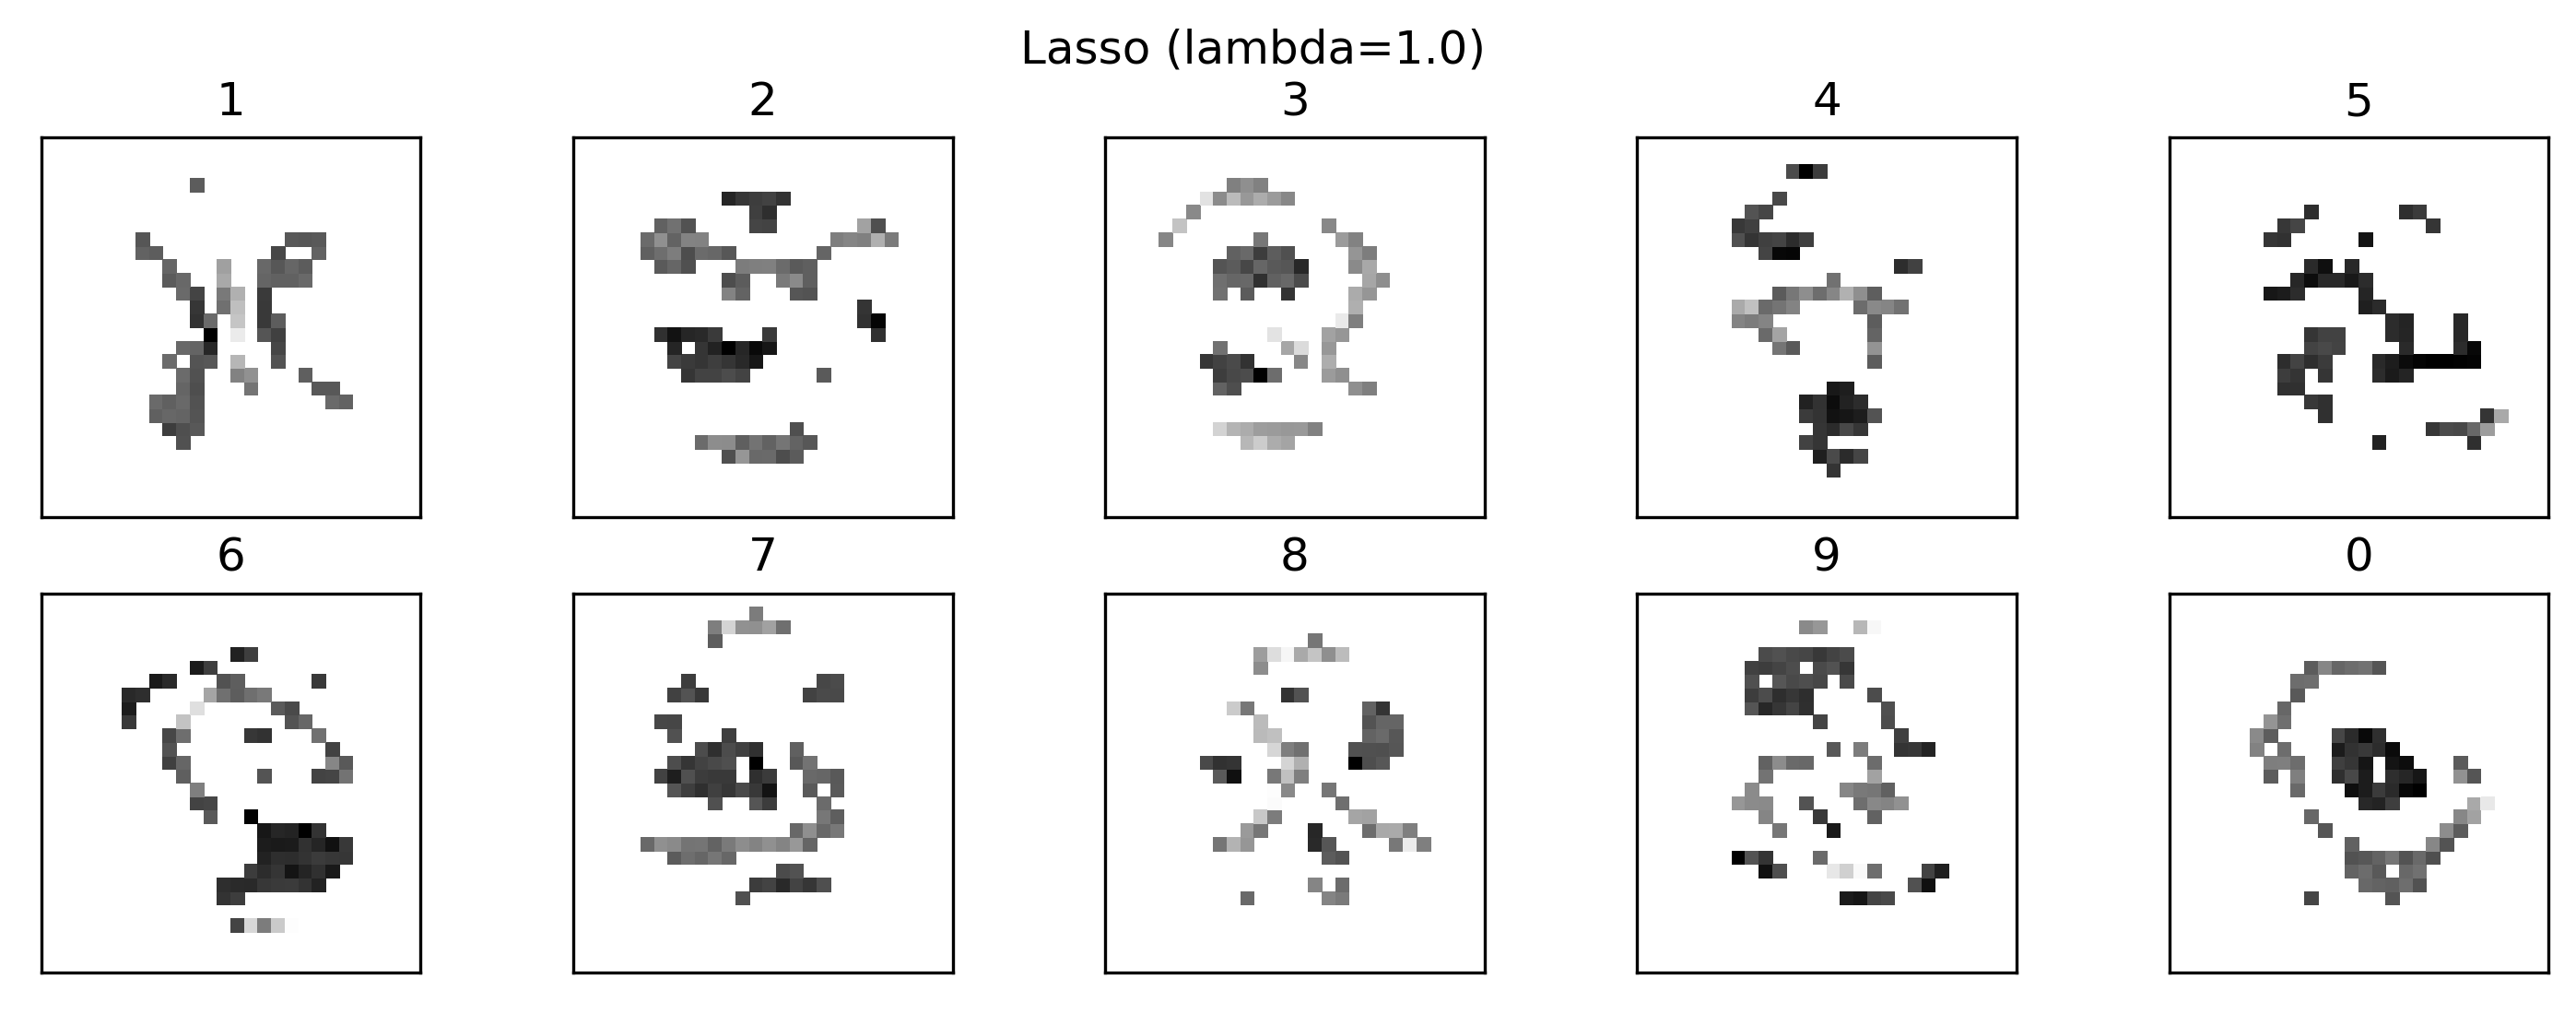
\includegraphics[scale=0.75]{figures/weight_matrix_lasso_1_no_zeros.png}}
\caption{Caption....}
\label{fig10}
\end{figure}

\begin{figure}[ht]
\centerline{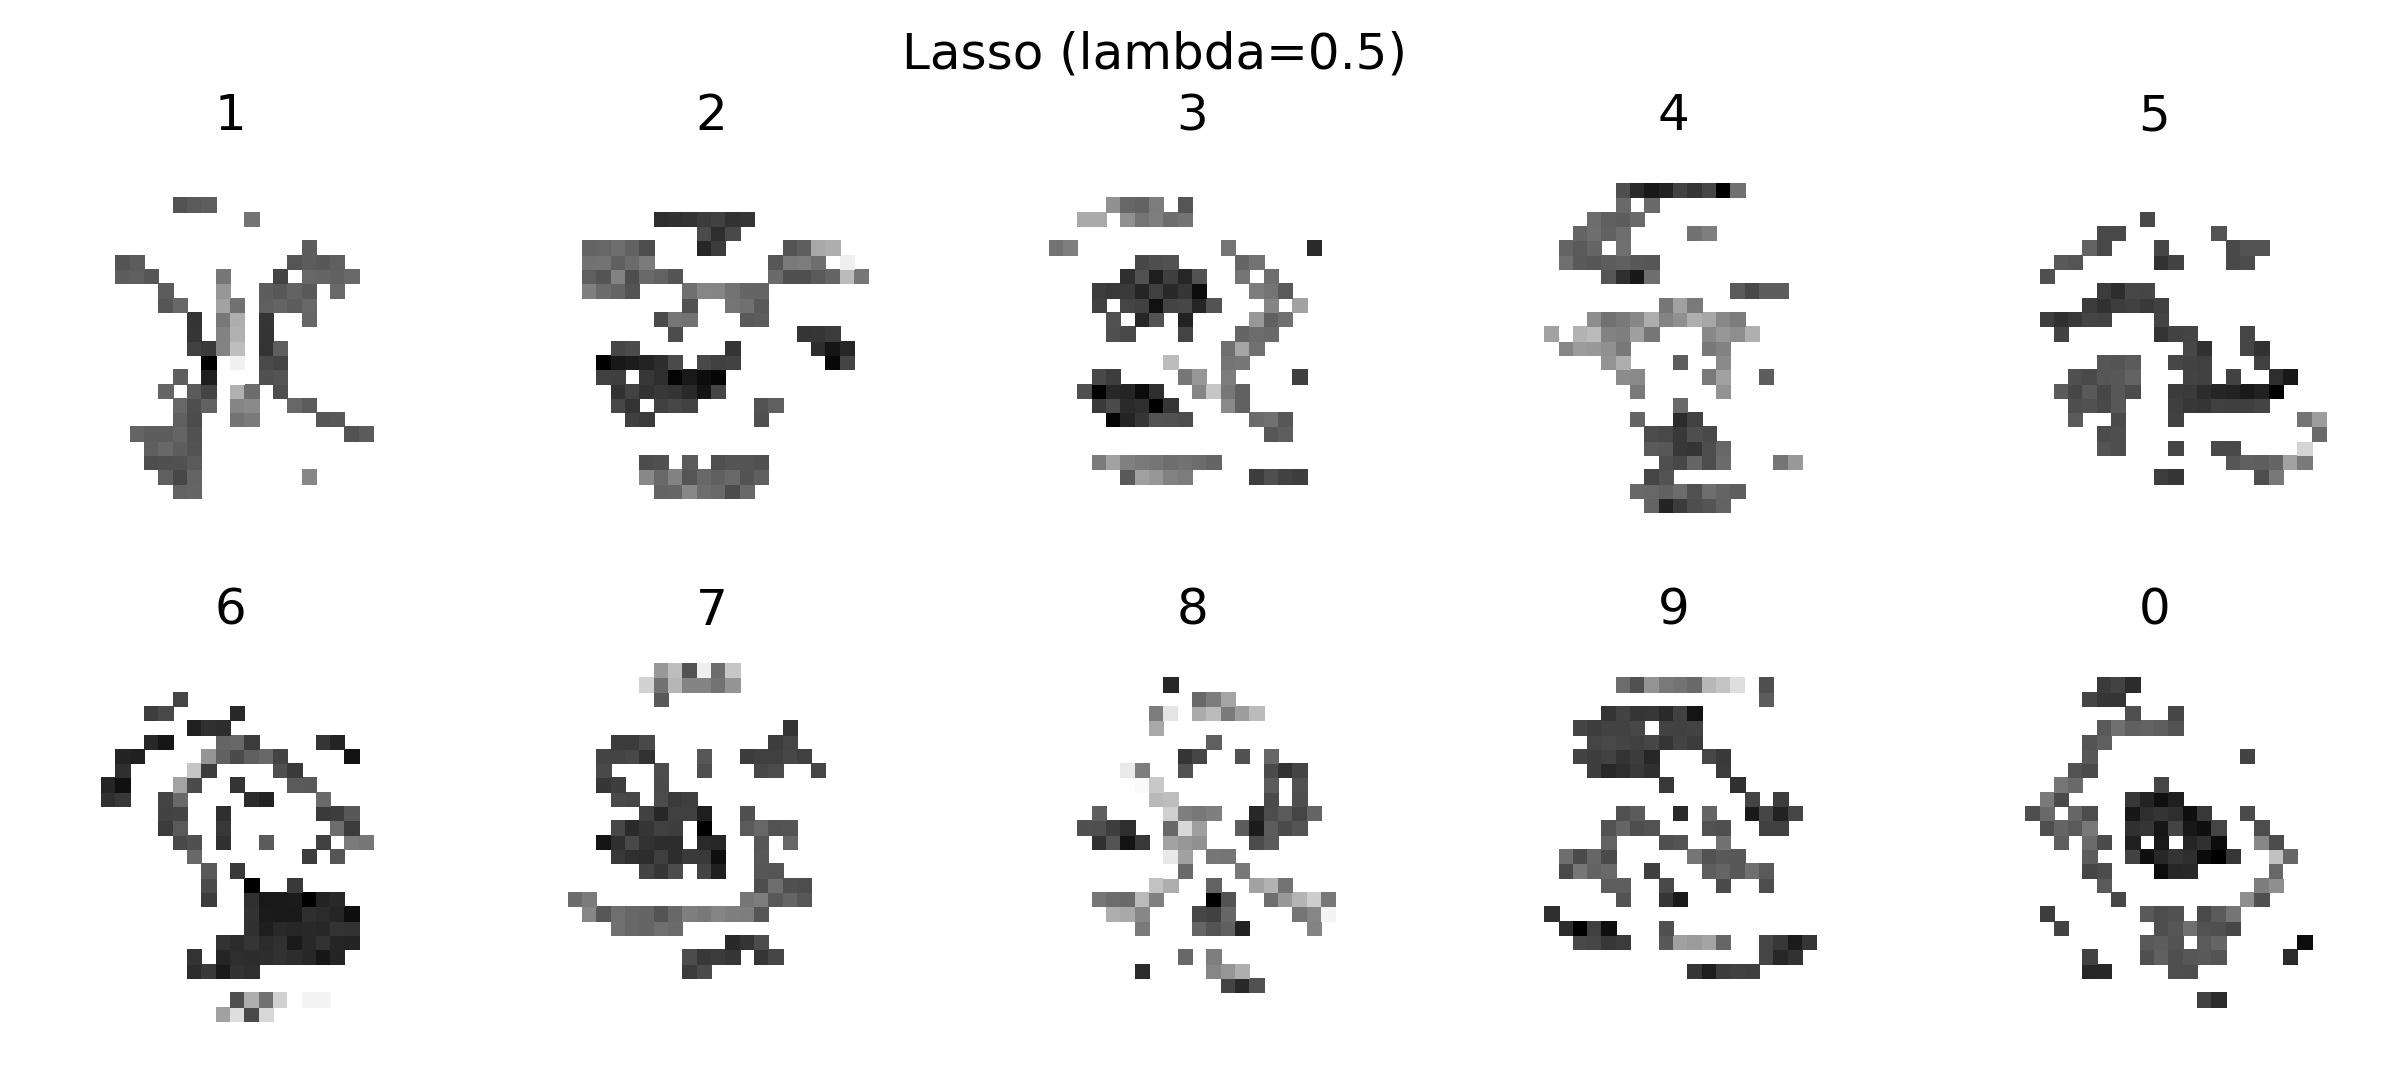
\includegraphics[scale=0.75]{figures/weight_matrix_lasso_05_no_zeros.png}}
\caption{Caption....}
\label{fig11}
\end{figure}

\begin{figure}[ht]
\centerline{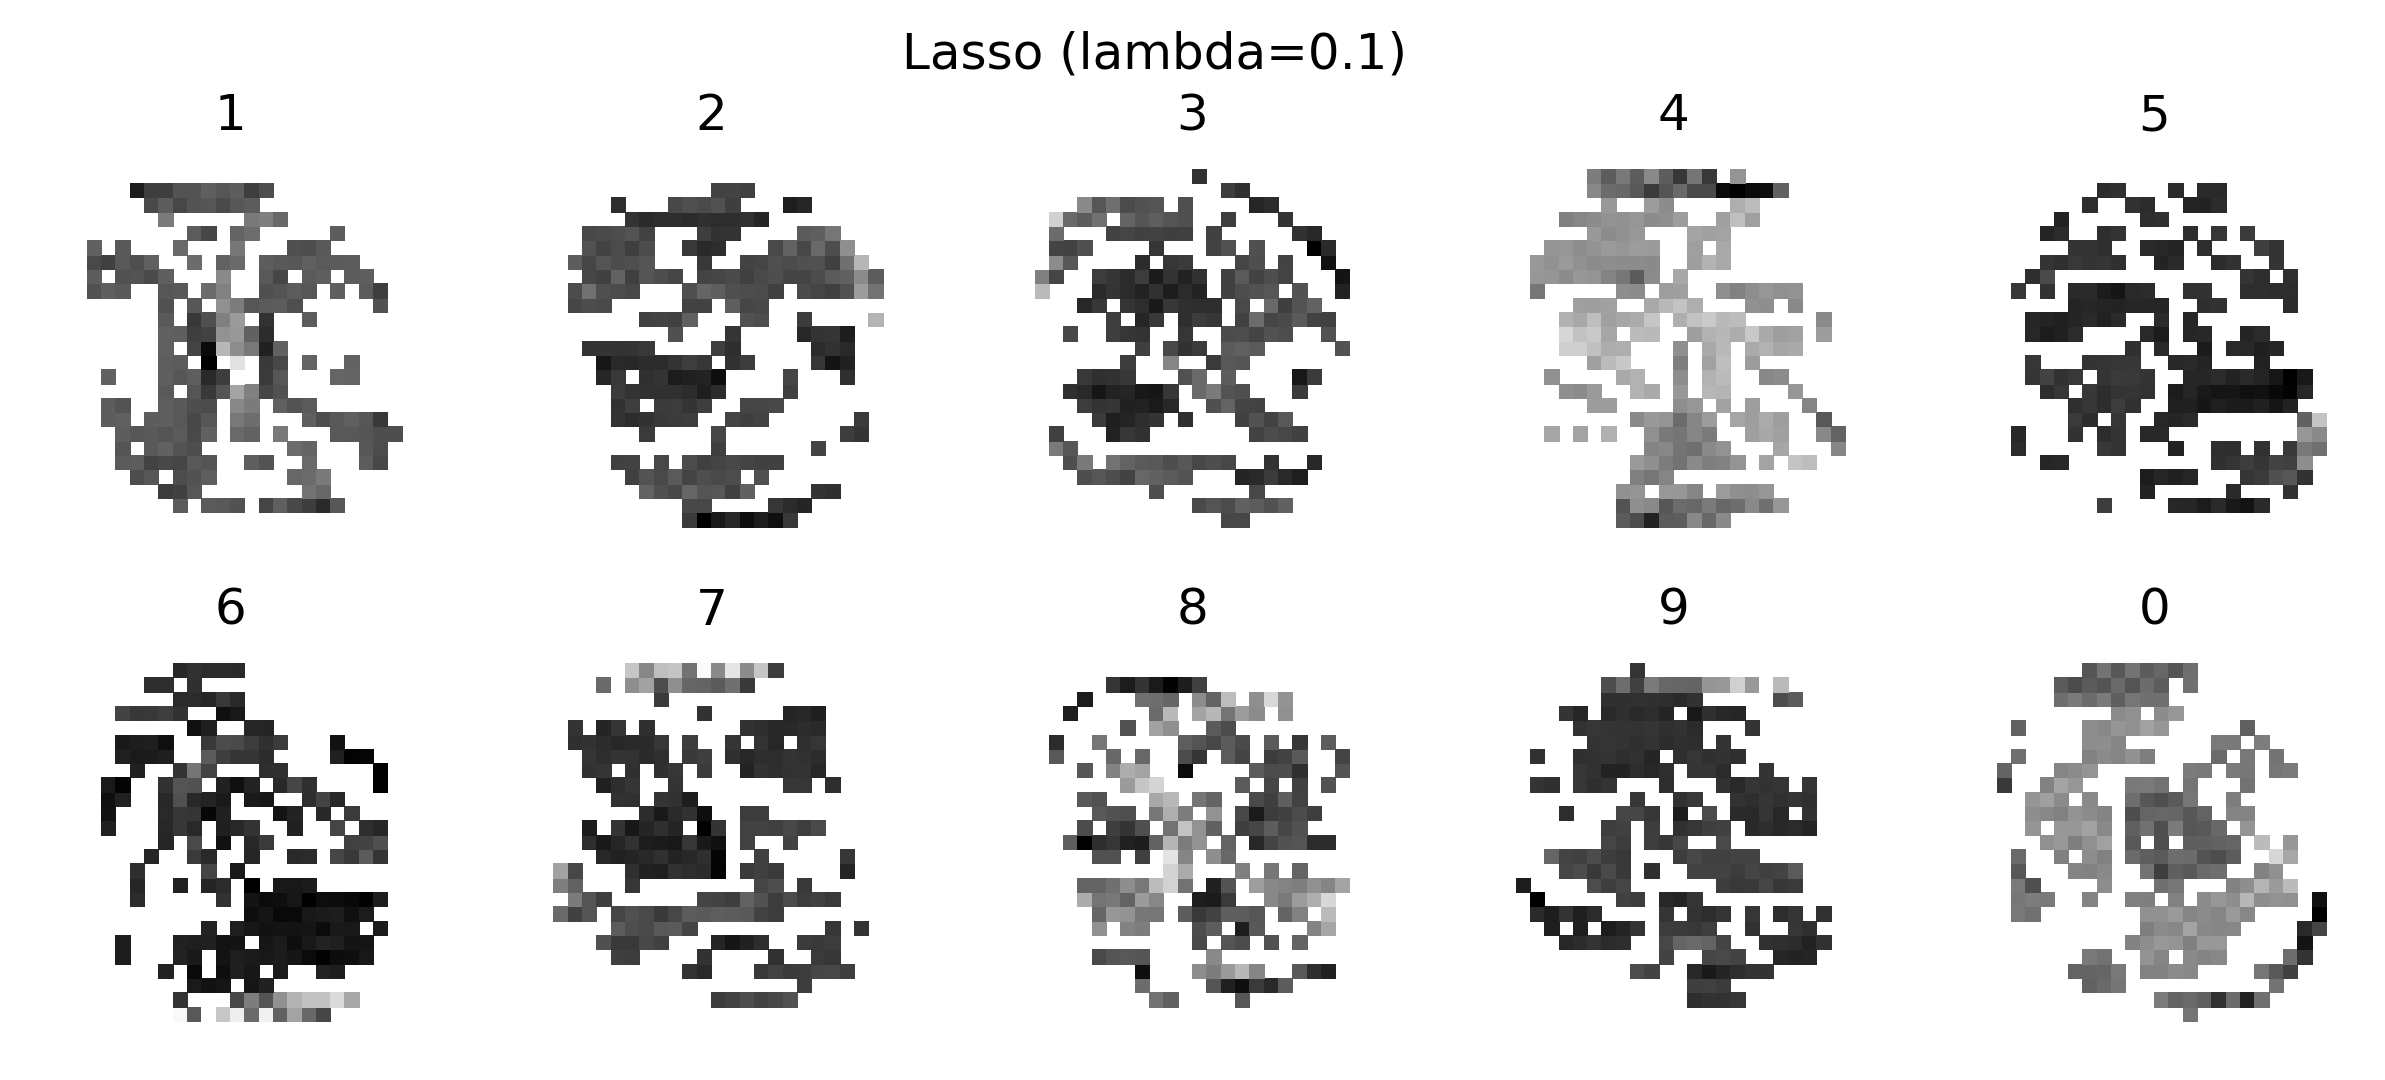
\includegraphics[scale=0.75]{figures/weight_matrix_lasso_01_no_zeros.png}}
\caption{Caption....}
\label{fig12}
\end{figure}

\begin{figure}[ht]
\centerline{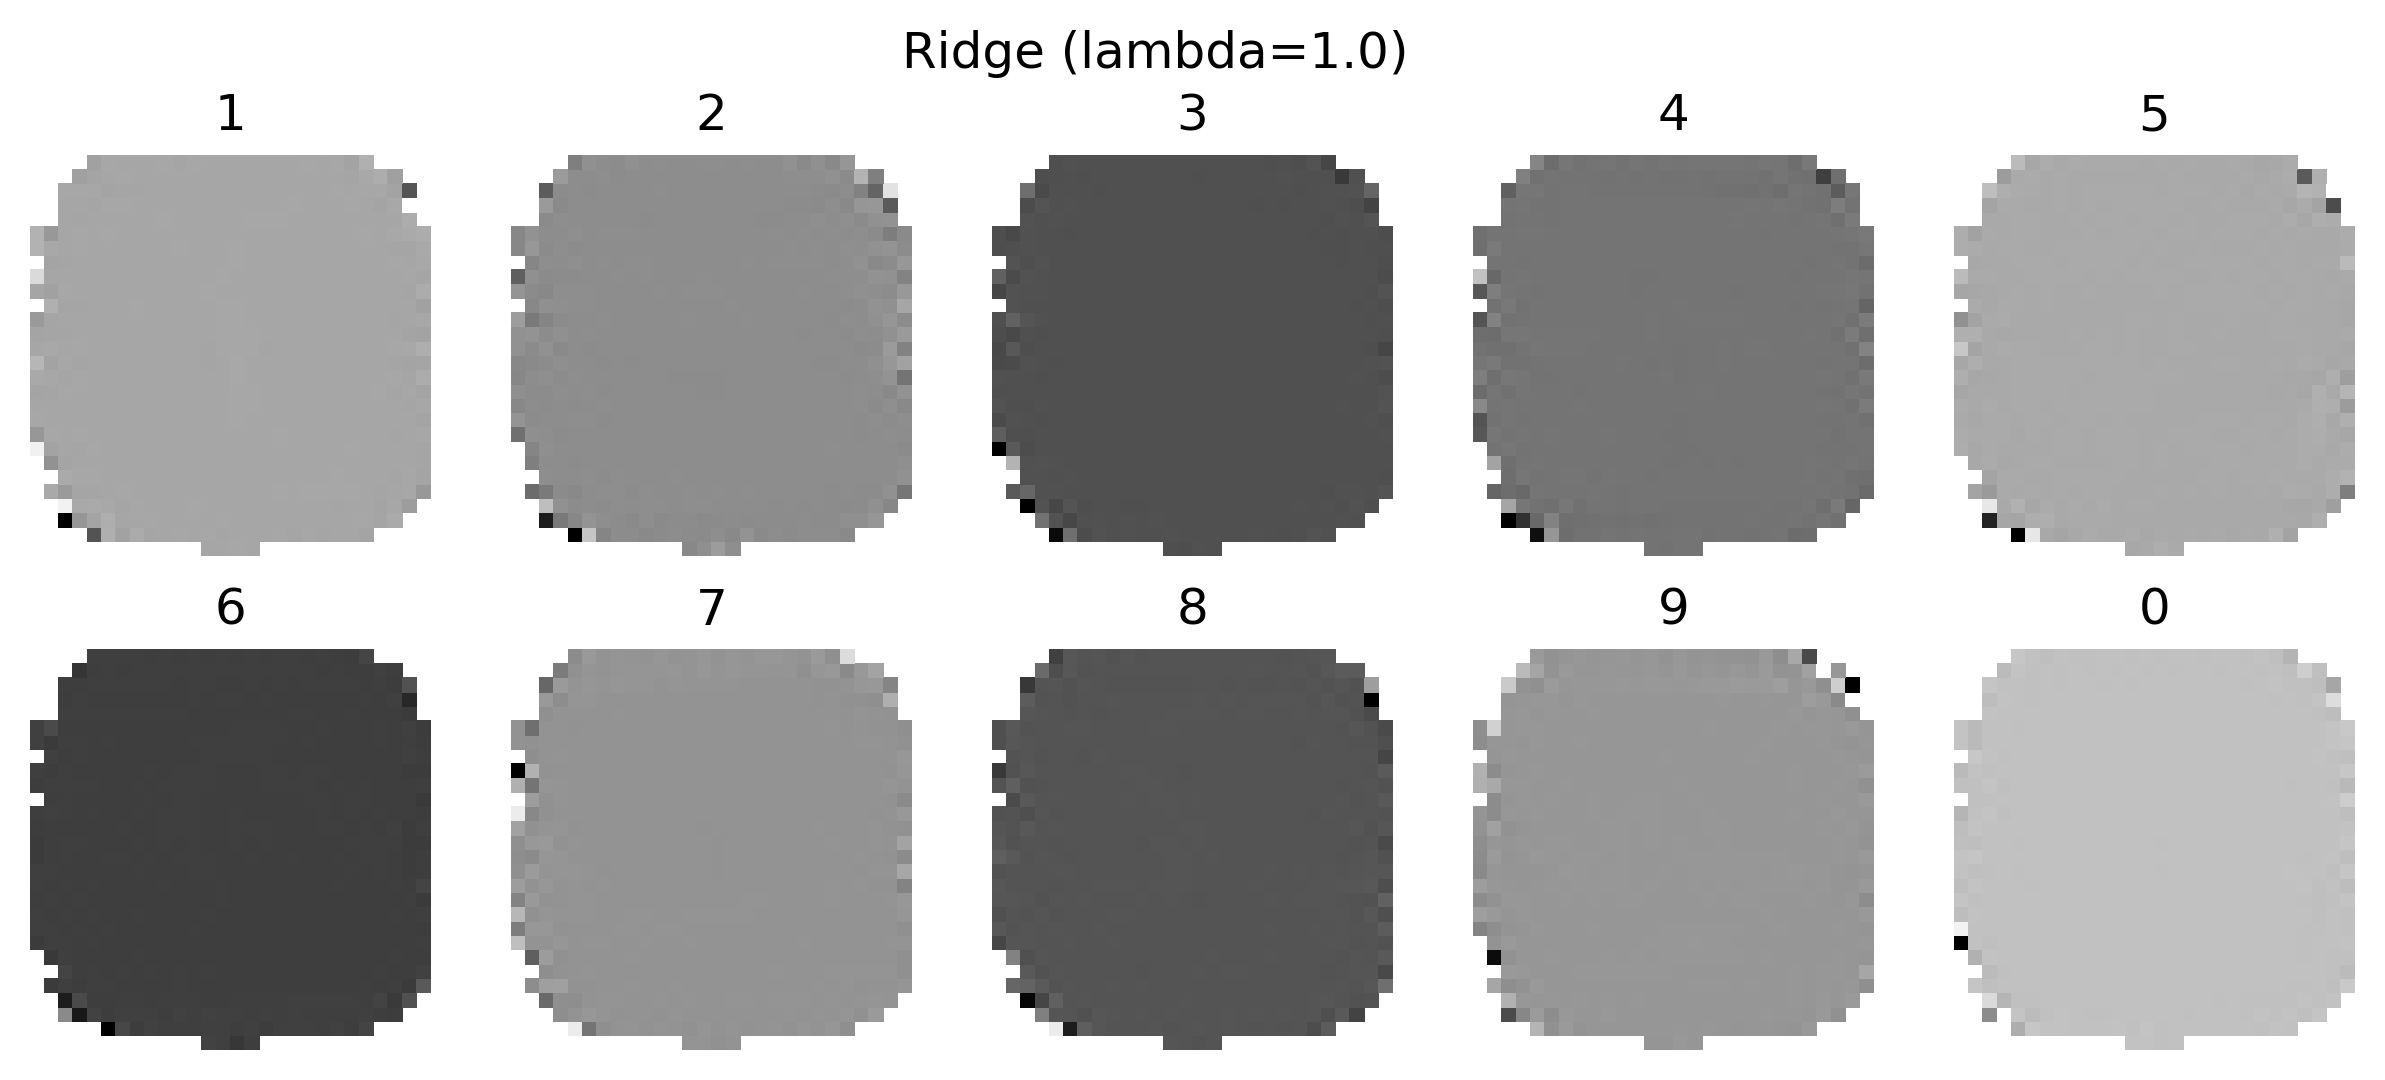
\includegraphics[scale=0.75]{figures/weight_matrix_ridge_no_zeros.png}}
\caption{Caption....}
\label{fig13}
\end{figure}

\begin{figure}[ht]
\centerline{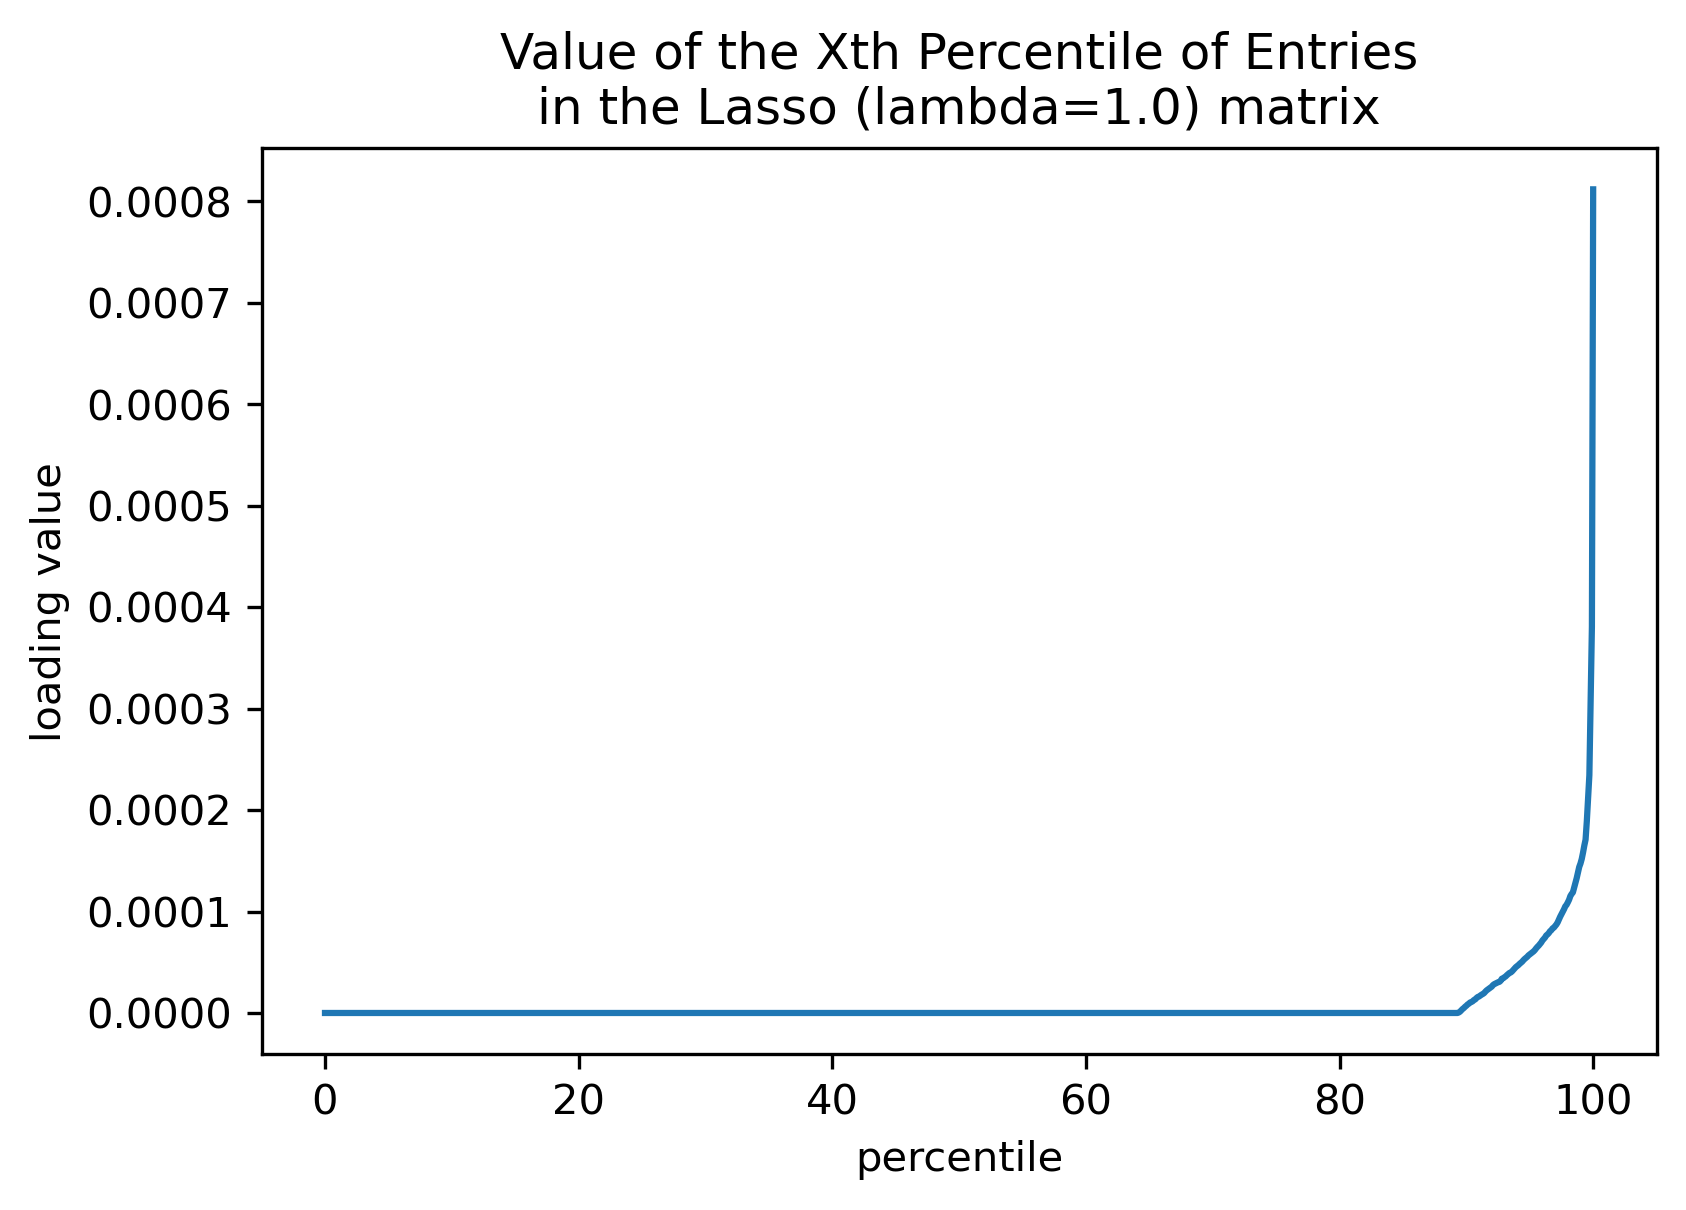
\includegraphics[scale=0.9]{figures/lasso_loading_percentiles-see_uptick_at_90.png}}
\caption{Caption....}
\label{fig14}
\end{figure}

\begin{figure}[ht]
\centerline{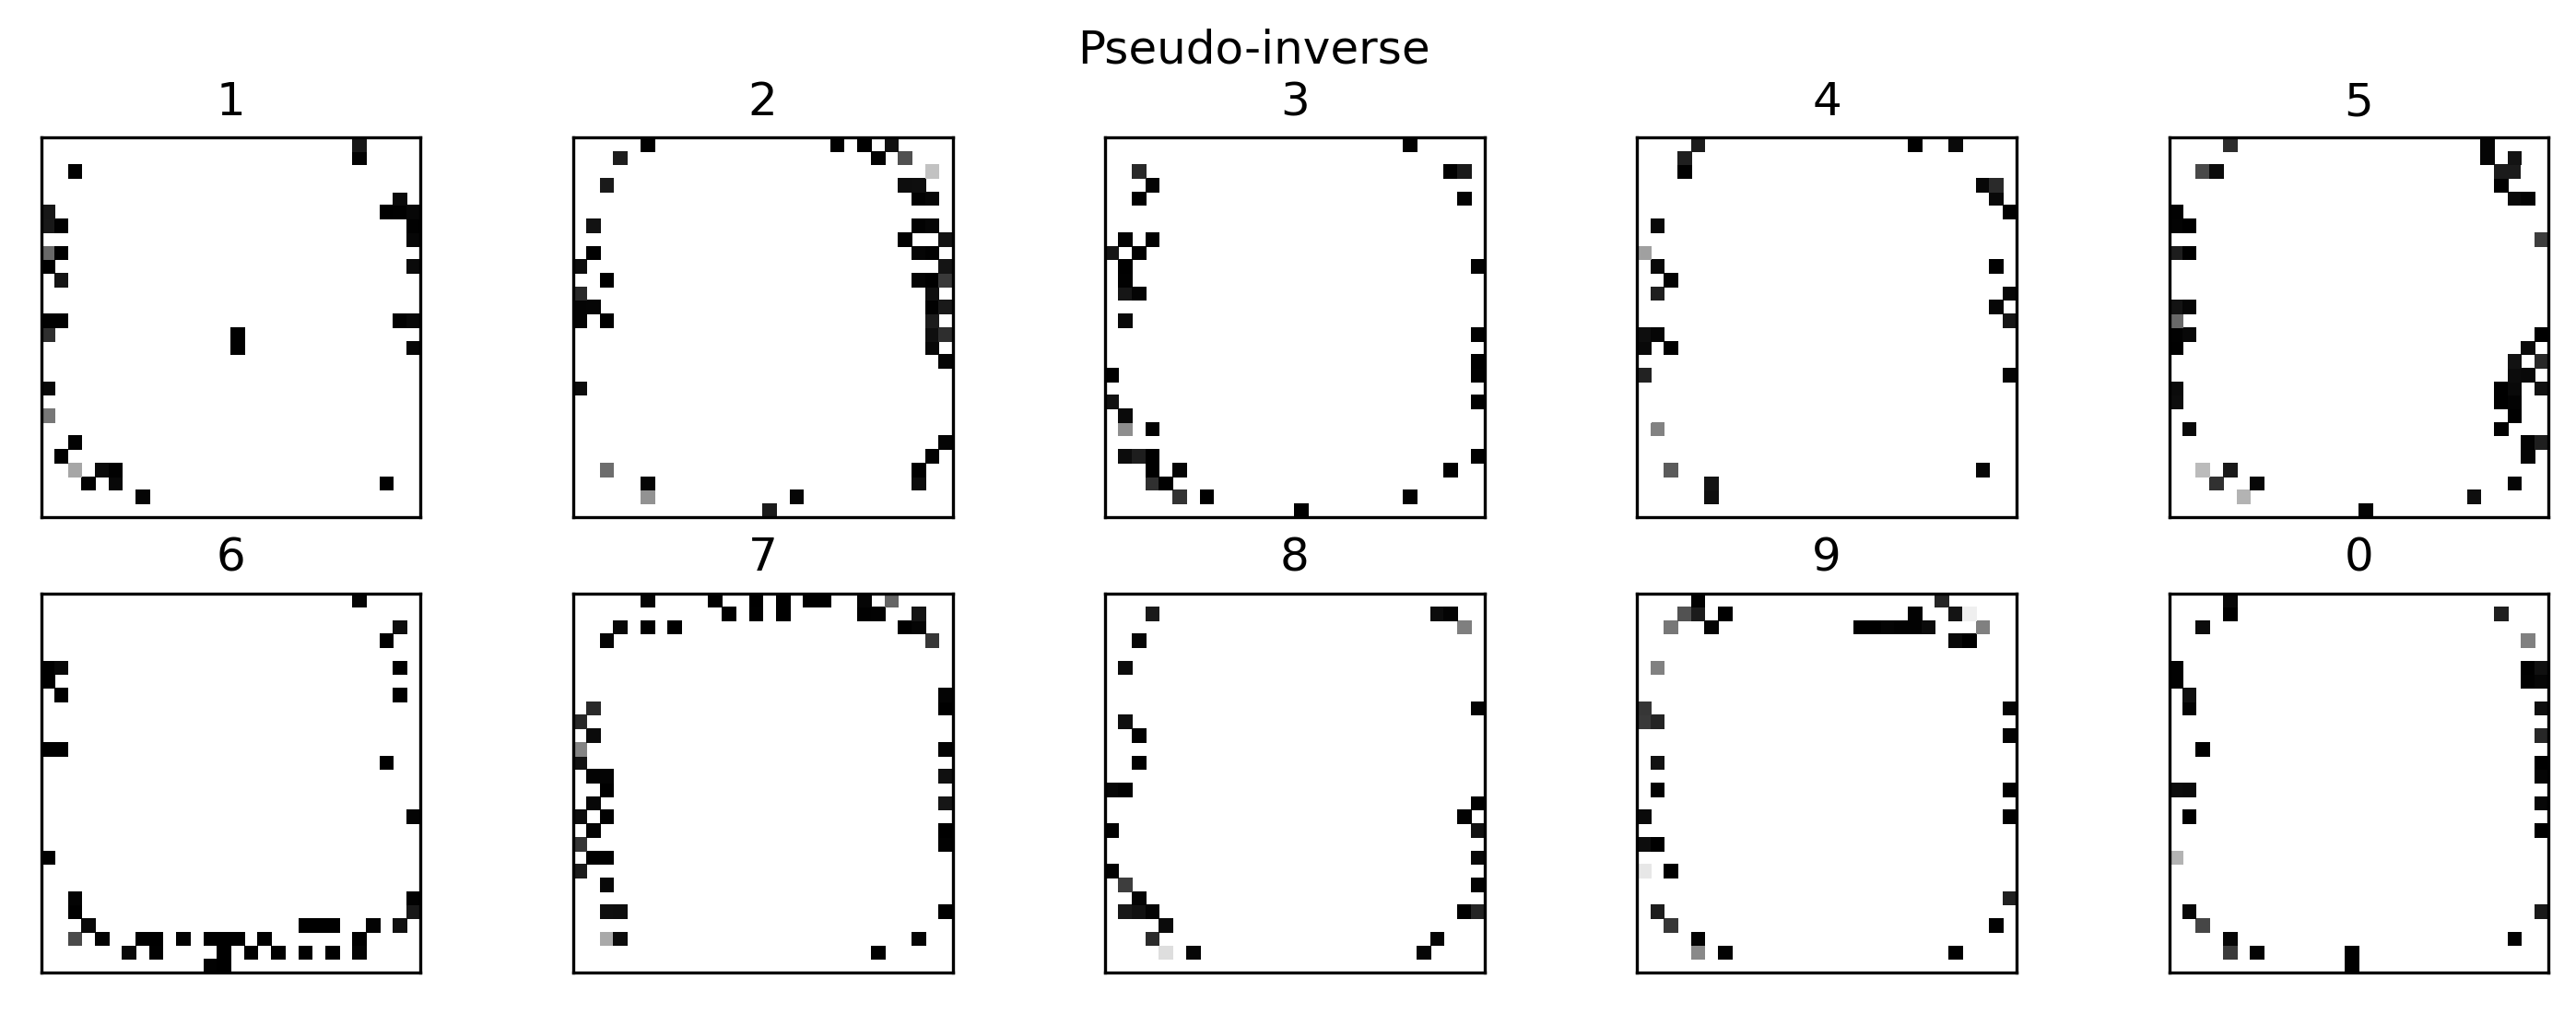
\includegraphics[scale=0.75]{figures/weight_matrix_pinv_geq_90th_no_zeros.png}}
\caption{Caption....}
\label{fig15}
\end{figure}

\begin{figure}[ht]
\centerline{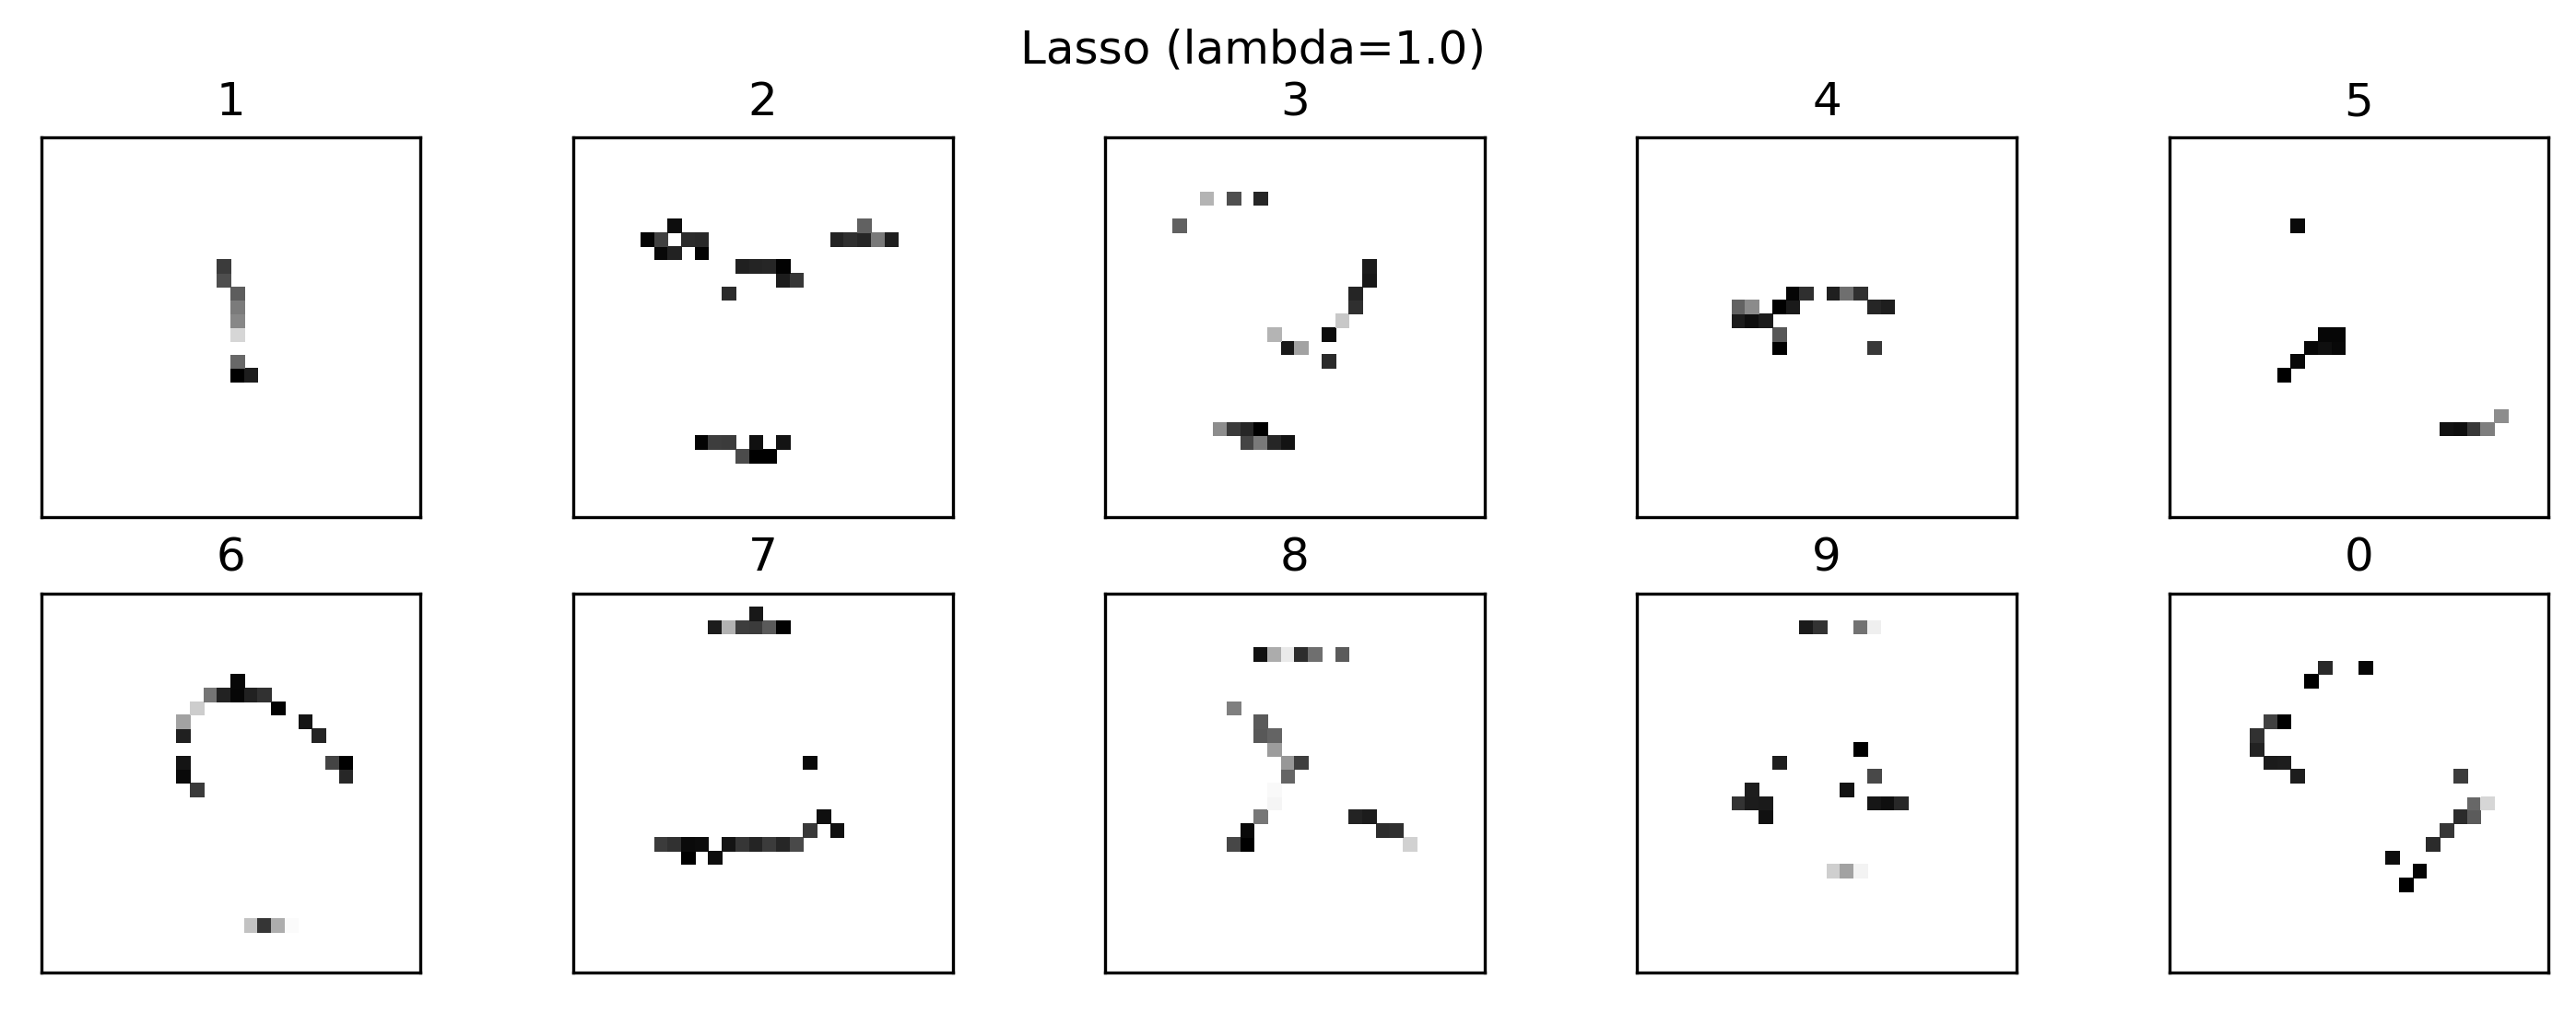
\includegraphics[scale=0.75]{figures/weight_matrix_lasso_1_geq_90th_no_zeros.png}}
\caption{Caption....}
\label{fig16}
\end{figure}

\begin{figure}[ht]
\centerline{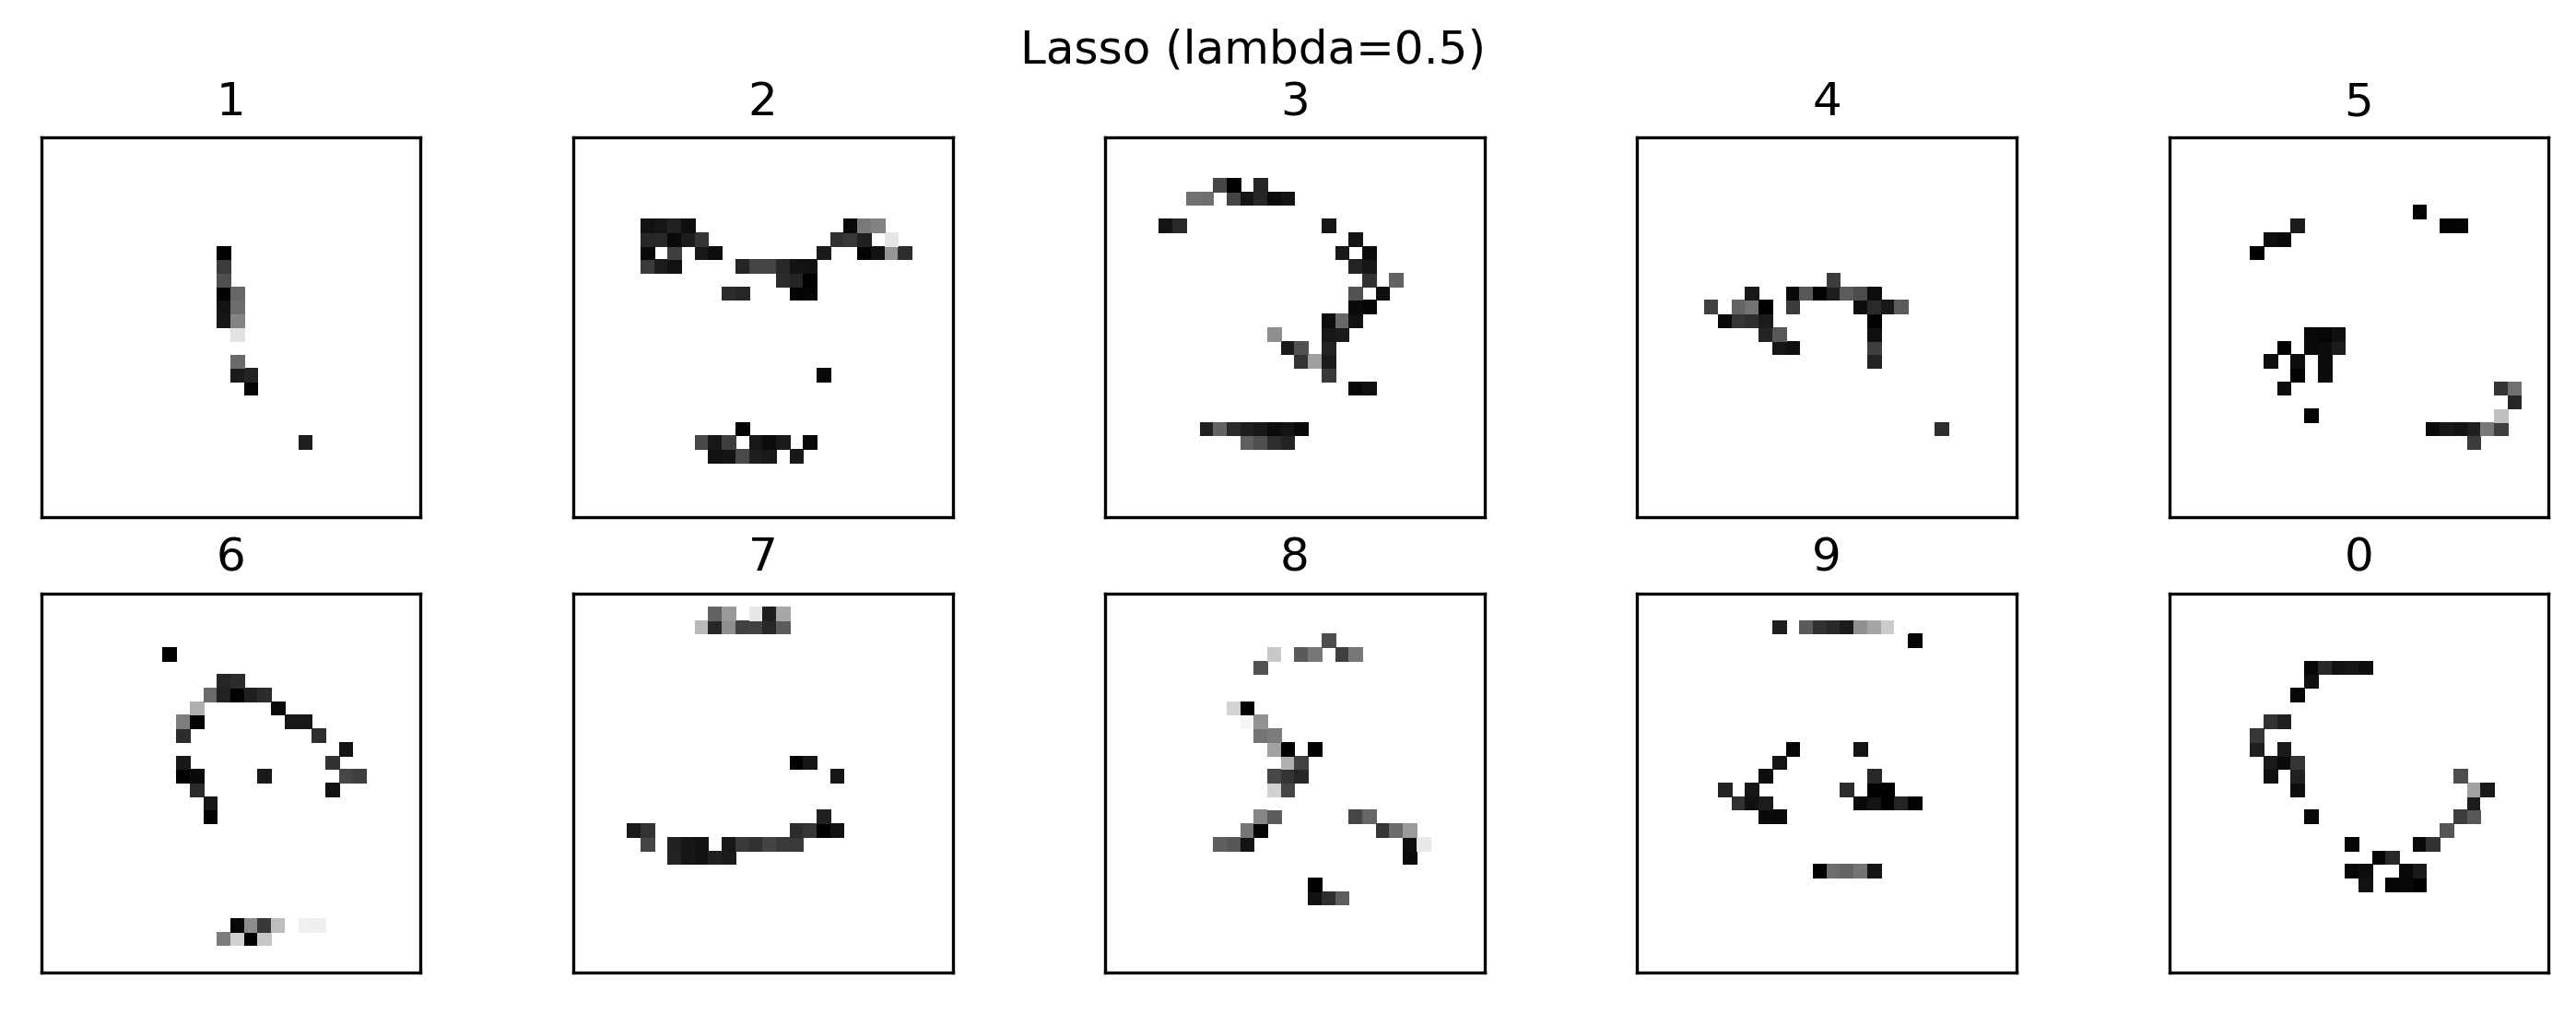
\includegraphics[scale=0.75]{figures/weight_matrix_lasso_05_geq_90th_no_zeros.png}}
\caption{Caption....}
\label{fig17}
\end{figure}

\begin{figure}[ht]
\centerline{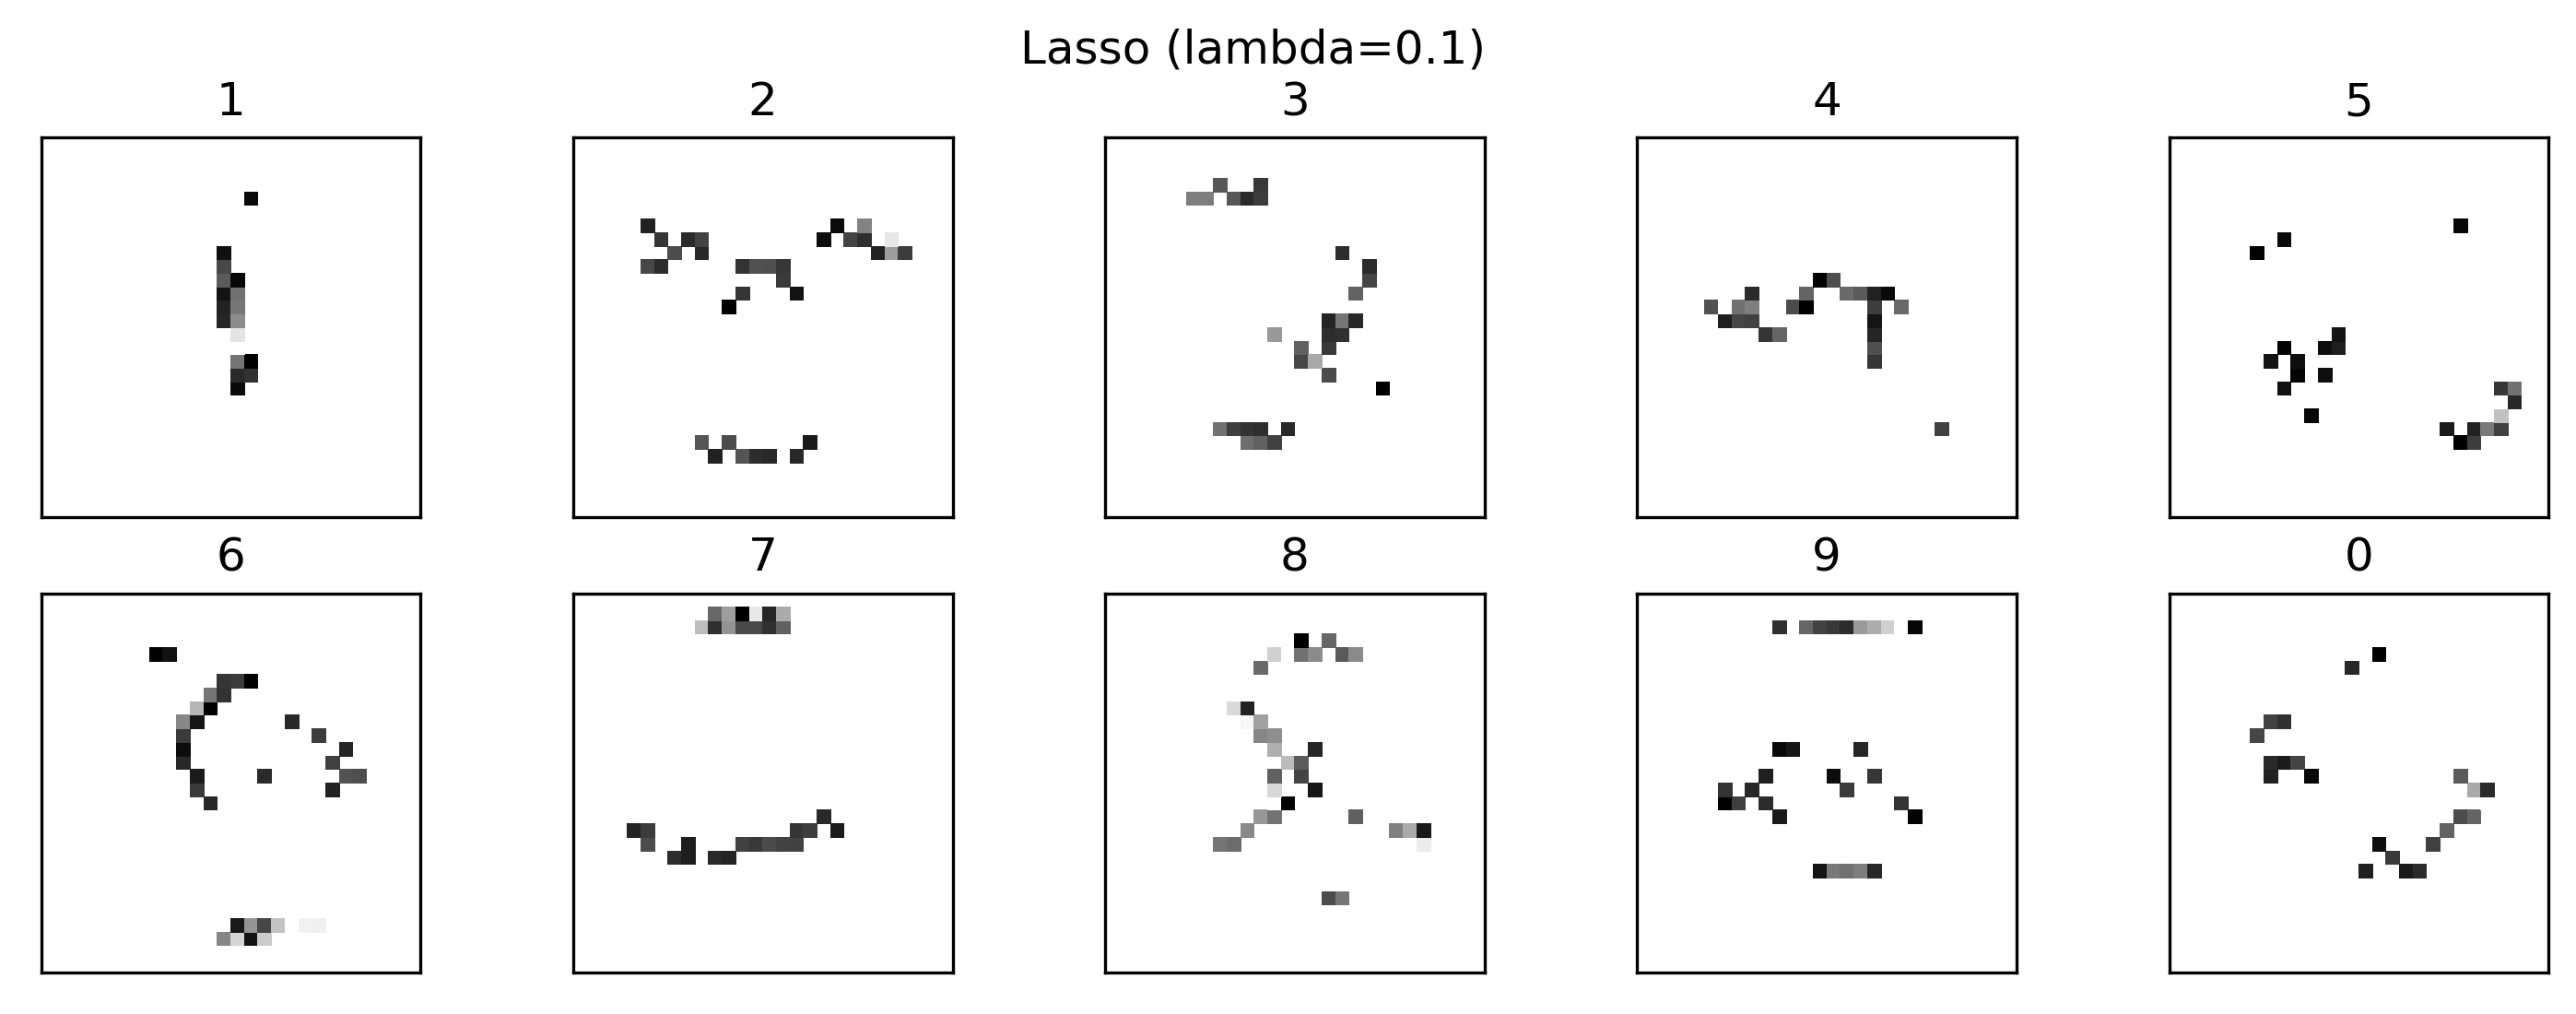
\includegraphics[scale=0.75]{figures/weight_matrix_lasso_01_geq_90th_no_zeros.png}}
\caption{Caption....}
\label{fig18}
\end{figure}

\begin{figure}[ht]
\centerline{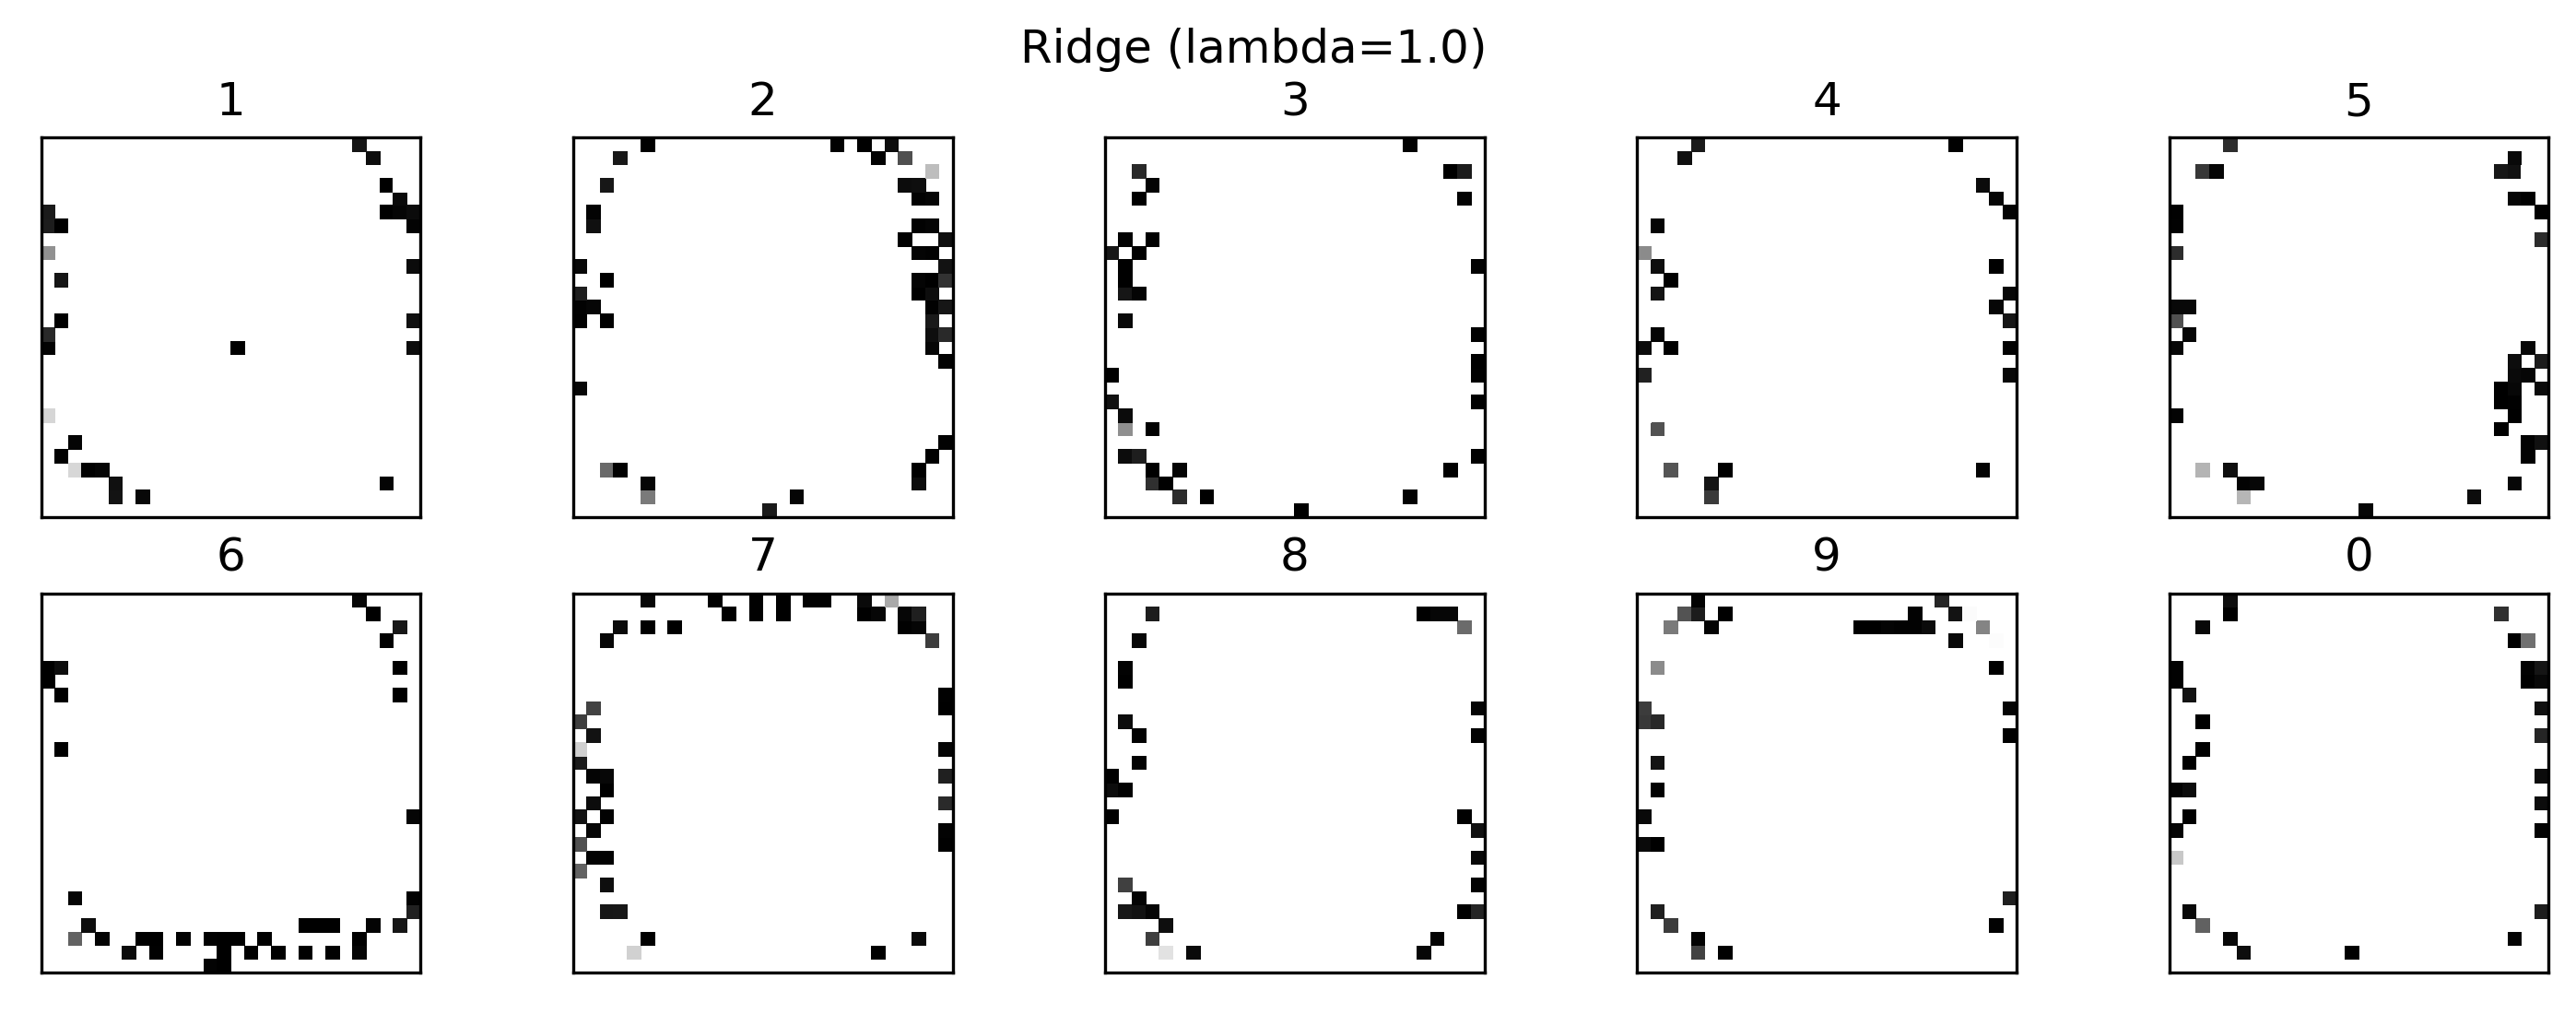
\includegraphics[scale=0.75]{figures/weight_matrix_ridge_geq_90th_no_zeros.png}}
\caption{Caption....}
\label{fig19}
\end{figure}

\begin{figure}[ht]
\centerline{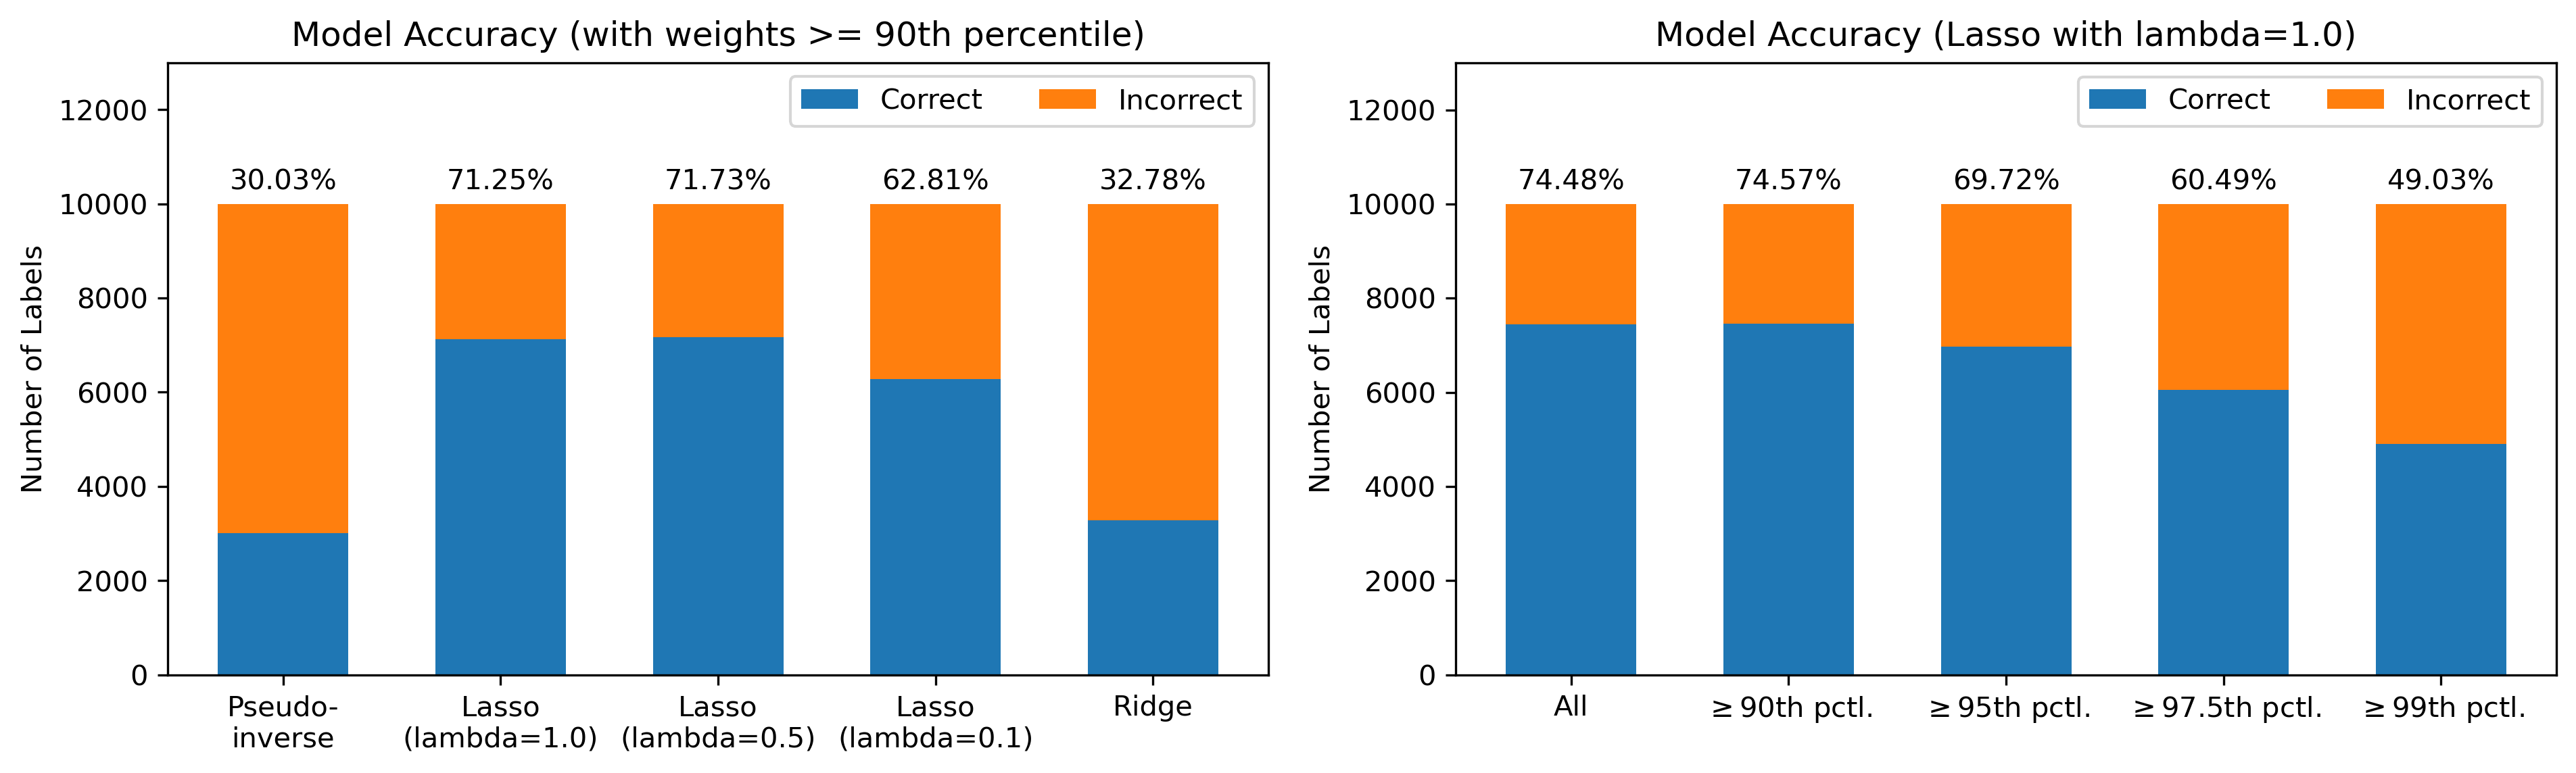
\includegraphics[scale=0.6]{figures/most_important_pixels_90th_accuracy.png}}
\caption{Caption....}
\label{fig20}
\end{figure}

\begin{figure}[ht]
\centerline{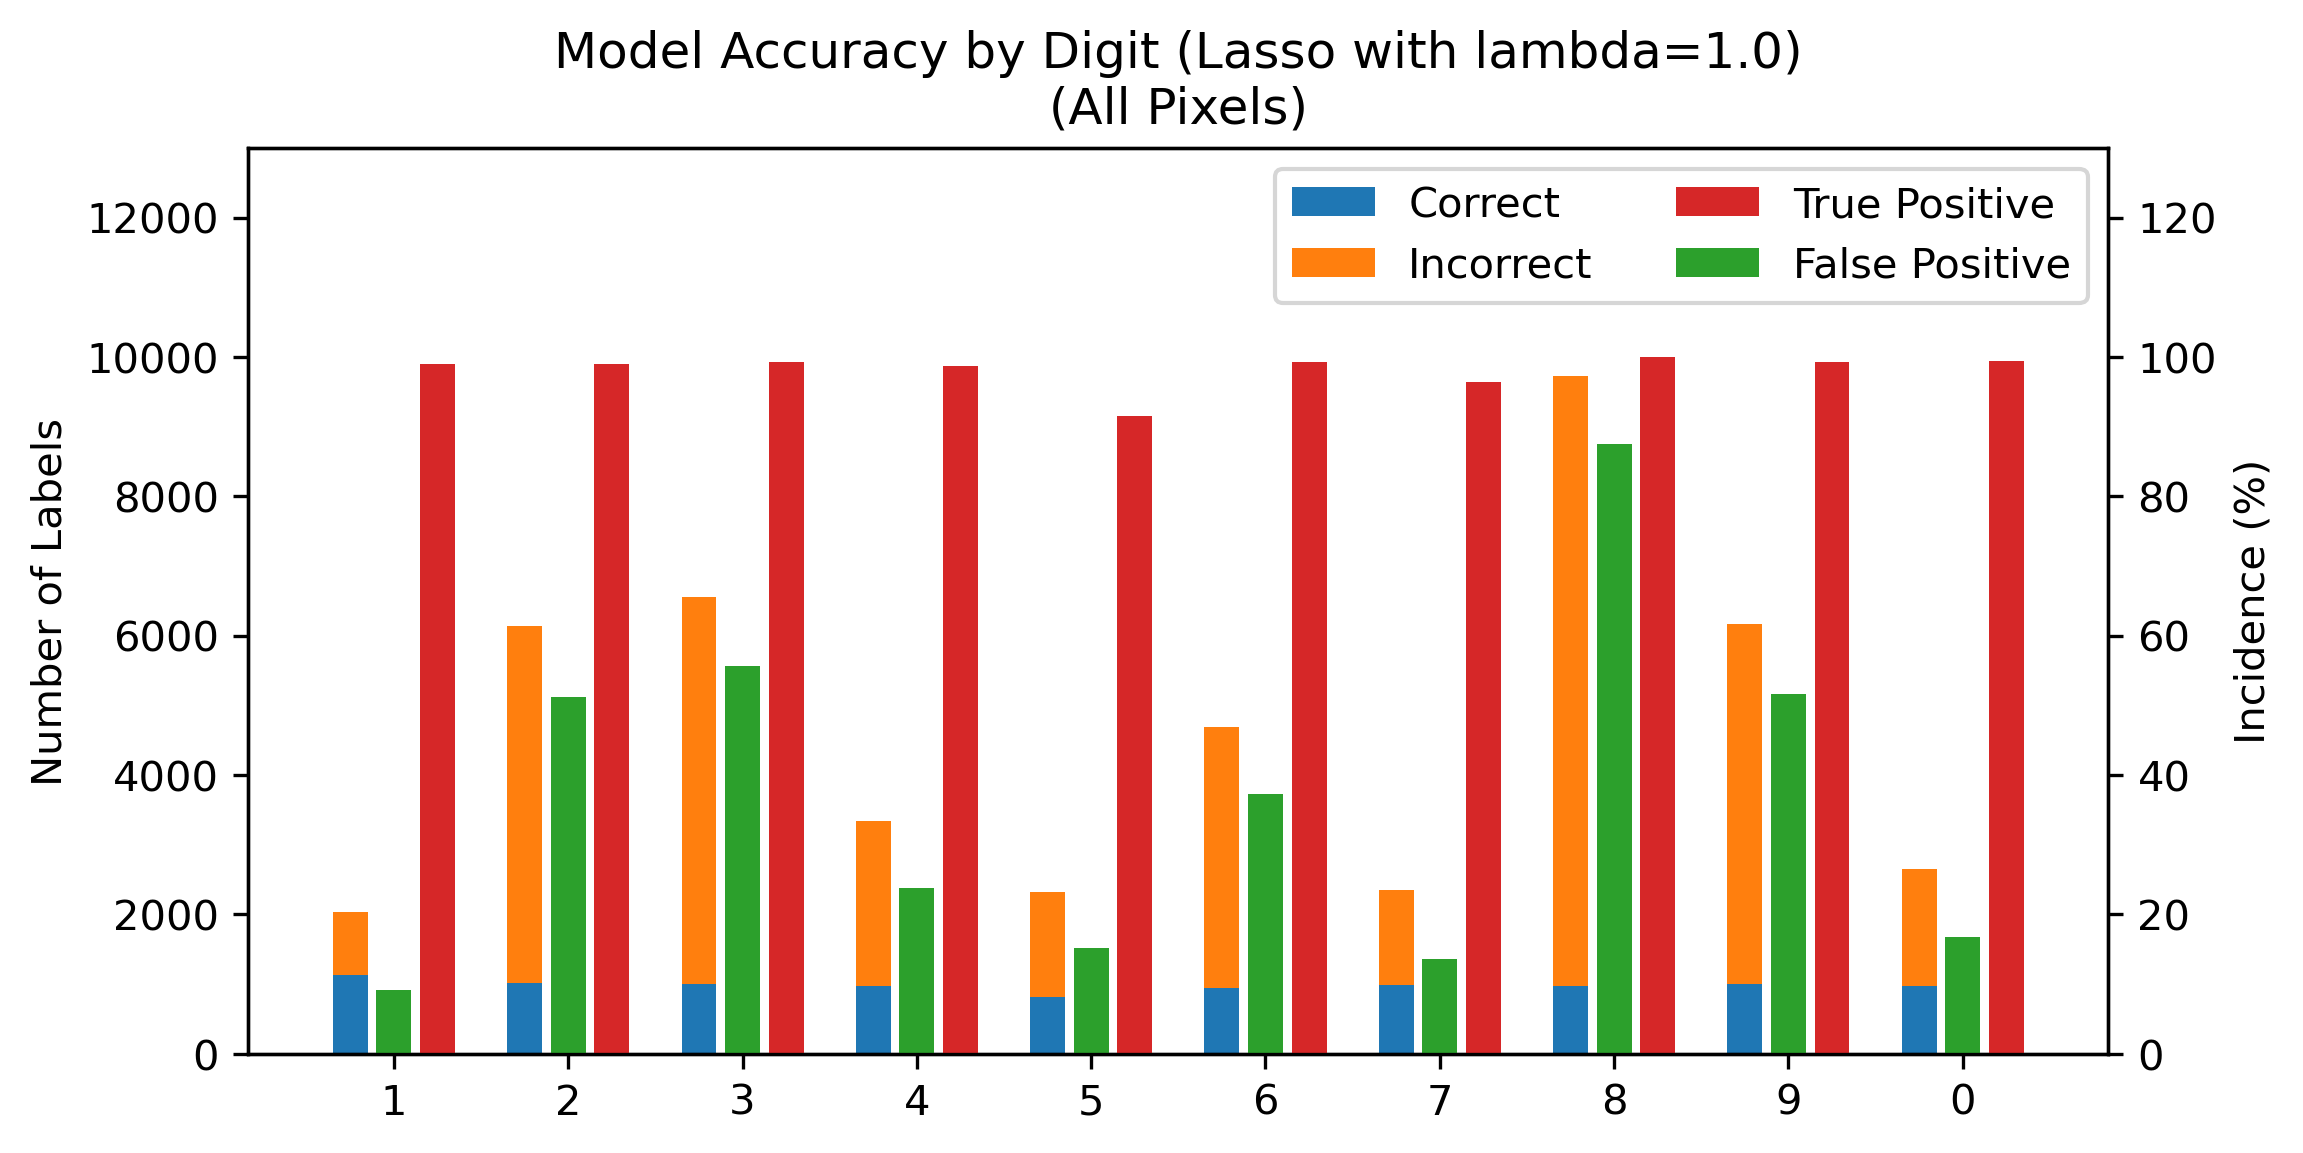
\includegraphics[scale=0.85]{figures/DIGIT_ALL_PIXELS_lasso_accuracy_comparison.png}}
\caption{Caption....}
\label{fig21}
\end{figure}

\begin{figure}[ht]
\centerline{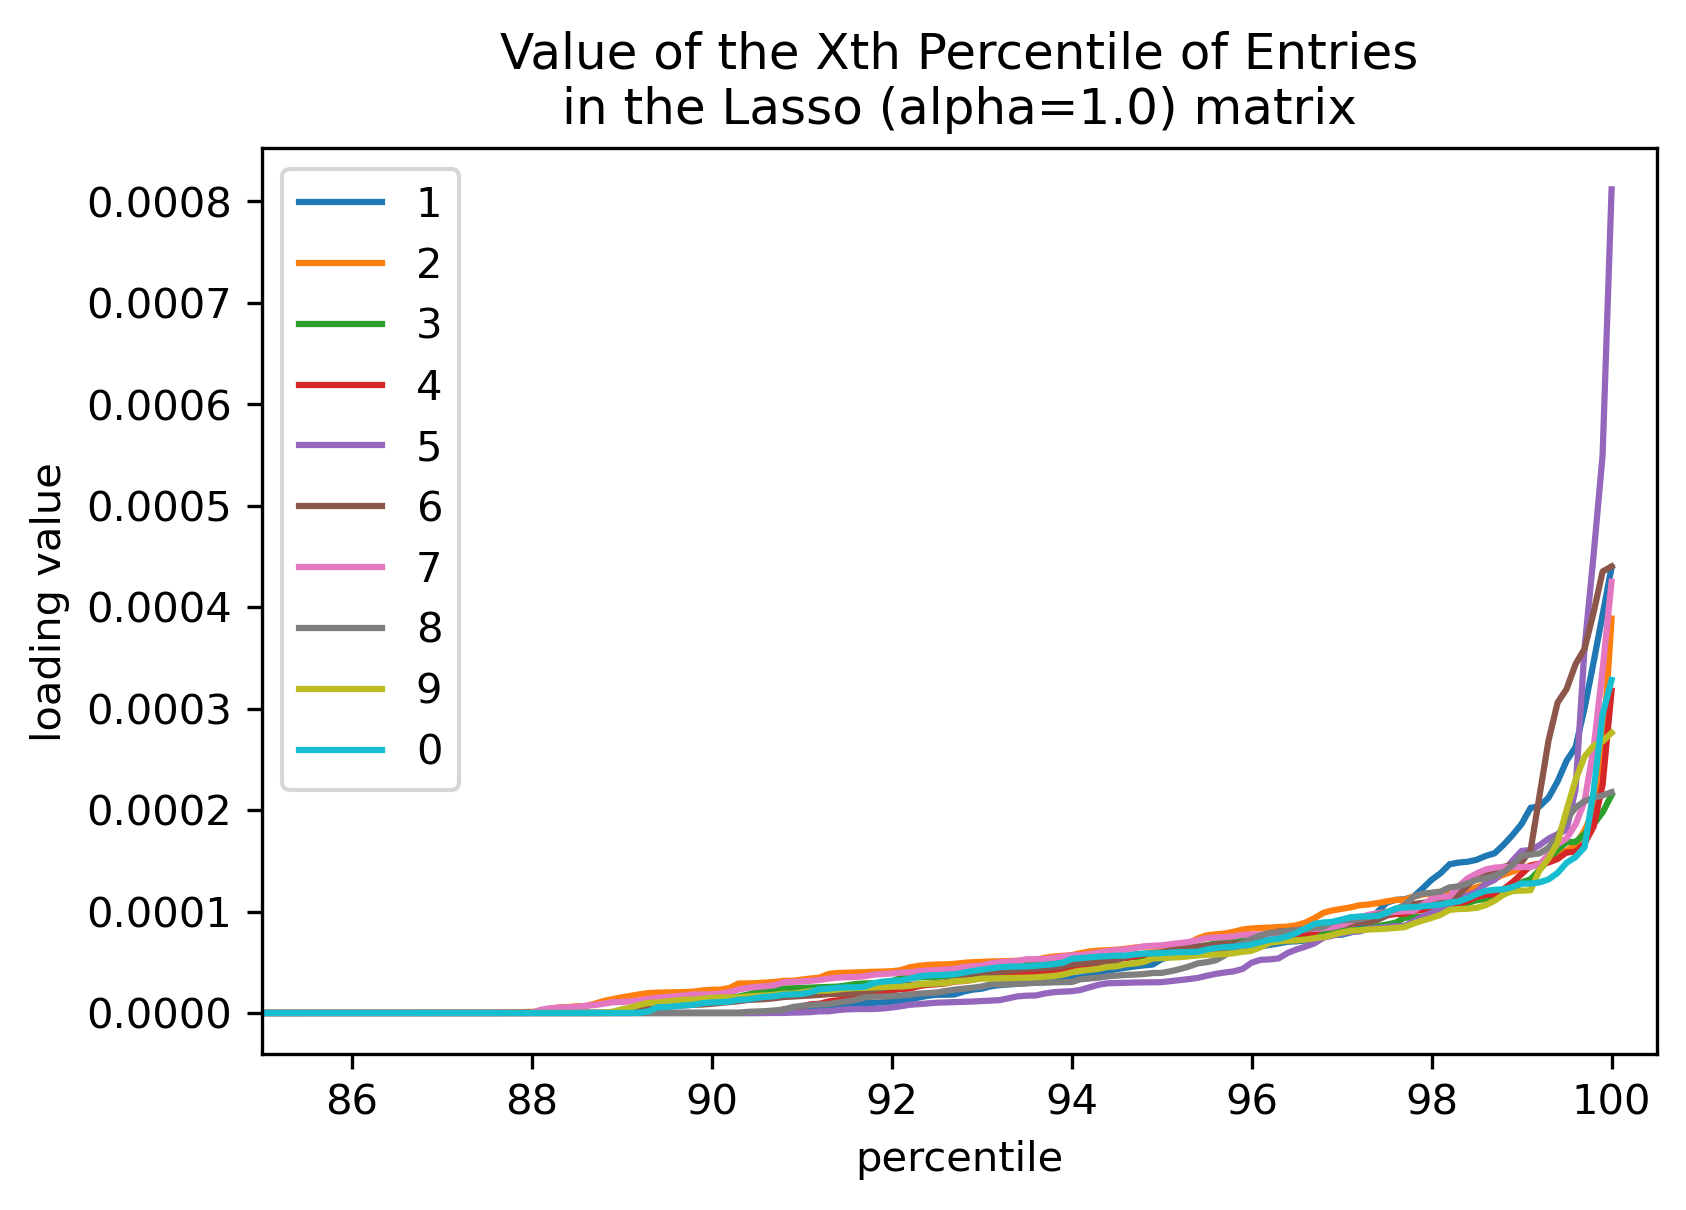
\includegraphics[scale=0.9]{figures/DIGIT_lasso_loading_percentiles-see_uptick_at_91.png}}
\caption{Caption....}
\label{fig22}
\end{figure}

\begin{figure}[ht]
\centerline{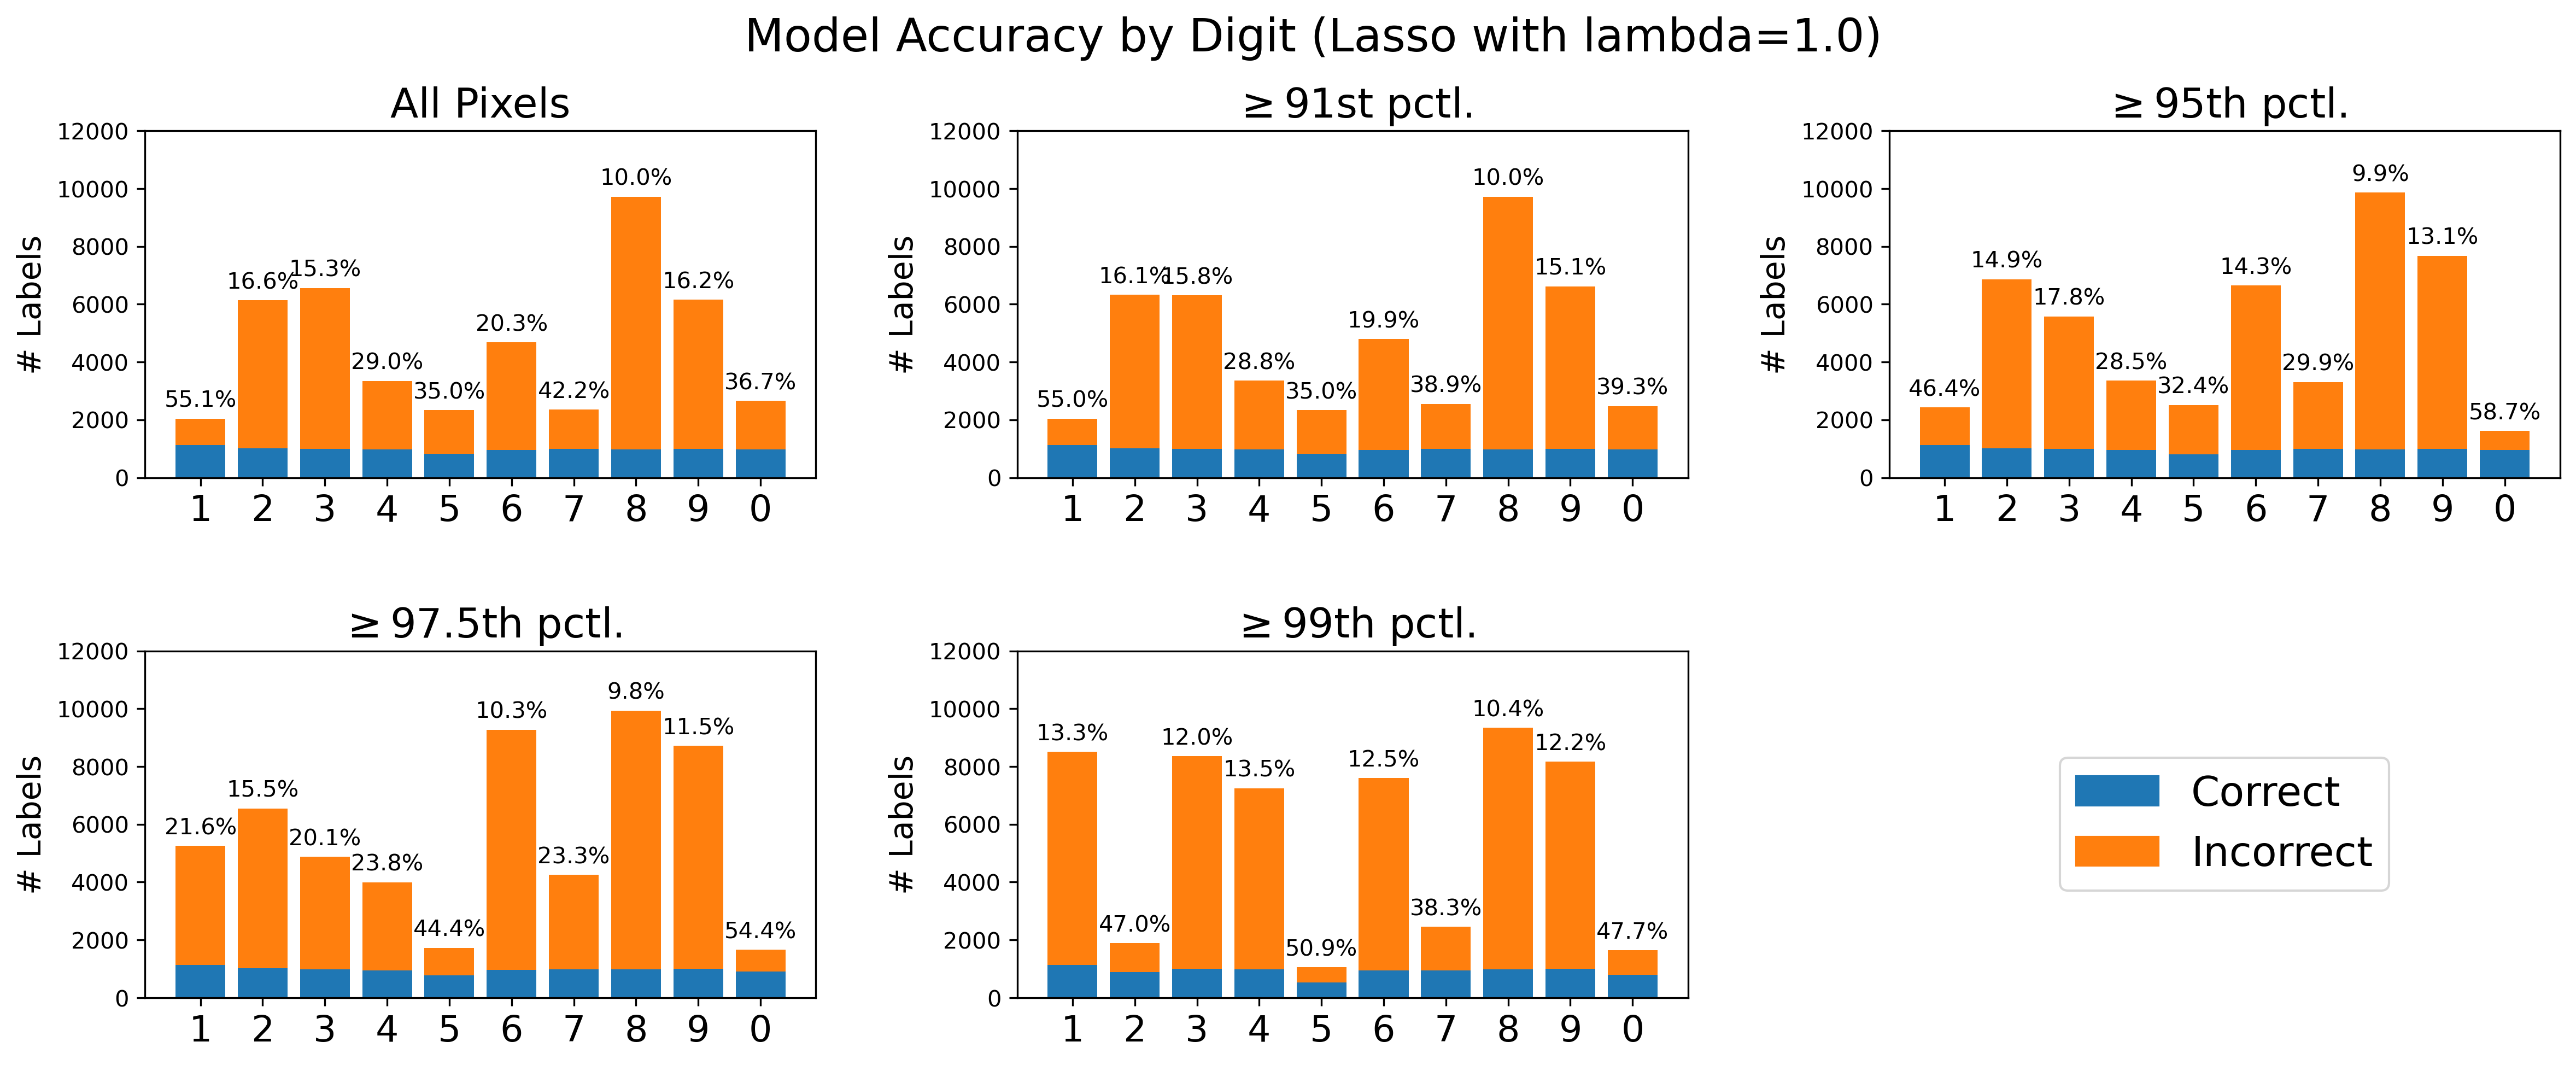
\includegraphics[scale=0.5]{figures/DIGIT_PCTS_lasso_accuracy_comparison.png}}
\caption{Caption....}
\label{fig23}
\end{figure}


\end{document}
